\documentclass[]{politex}
% ========== Opções ==========
% pnumromarab - Numeração de páginas usando algarismos romanos na parte pré-textual e arábicos na parte textual
% abnttoc - Forçar paginação no sumário conforme ABNT (inclui "p." na frente das páginas)
% normalnum - Numeração contínua de figuras e tabelas 
%	(caso contrário, a numeração é reiniciada a cada capítulo)
\label{key}% draftprint - Ajusta as margens para impressão de rascunhos
%	(reduz a margem interna)
% twosideprint - Ajusta as margens para impressão frente e verso
% capsec - Forçar letras maiúsculas no título das seções
% espacosimples - Documento usando espaçamento simples
% espacoduplo - Documento usando espaçamento duplo
%	(o padrão é usar espaçamento 1.5)
% times - Tenta usar a fonte Times New Roman para o corpo do texto
% noindentfirst - Não indenta o primeiro parágrafo dos capítulos/seções
% ========== Opções do documento ==========
% Título
\titulo{Título do texto}
\versao{Corrigida}
% Autor
\autor{Nome do autor}

% Para múltiplos autores (TCC)
%\autor{Nome Sobrenome\\%
%		Nome Sobrenome\\%
%		Nome Sobrenome}

% Orientador / Coorientador
\orientador{Nome do Orientador}

%\coorientador{Nome do coorientador (opcional)}

% Tipo de documento
%\tcc{Engenheiro Civil}
\dissertacao{Ciências}
%\teseDOC{Engenharia Transportes}
%\teseLD
%\memorialLD

% Departamento e área de concentração
\departamento{Departamento de Engenharia de Transportes}
\areaConcentracao{Engenharia de Transportes}

% Local
\local{São Paulo}

% Ano
\data{2020}

\begin{document}
% ========== Capa e folhas de rosto ==========
\capa
\falsafolhaderosto
\folhaderosto
% ========== Ficha catalográfica ==========
% Fazer solicitação no site:
%	http://www.poli.usp.br/en/bibliotecas/servicos/catalogacao-na-publicacao.html

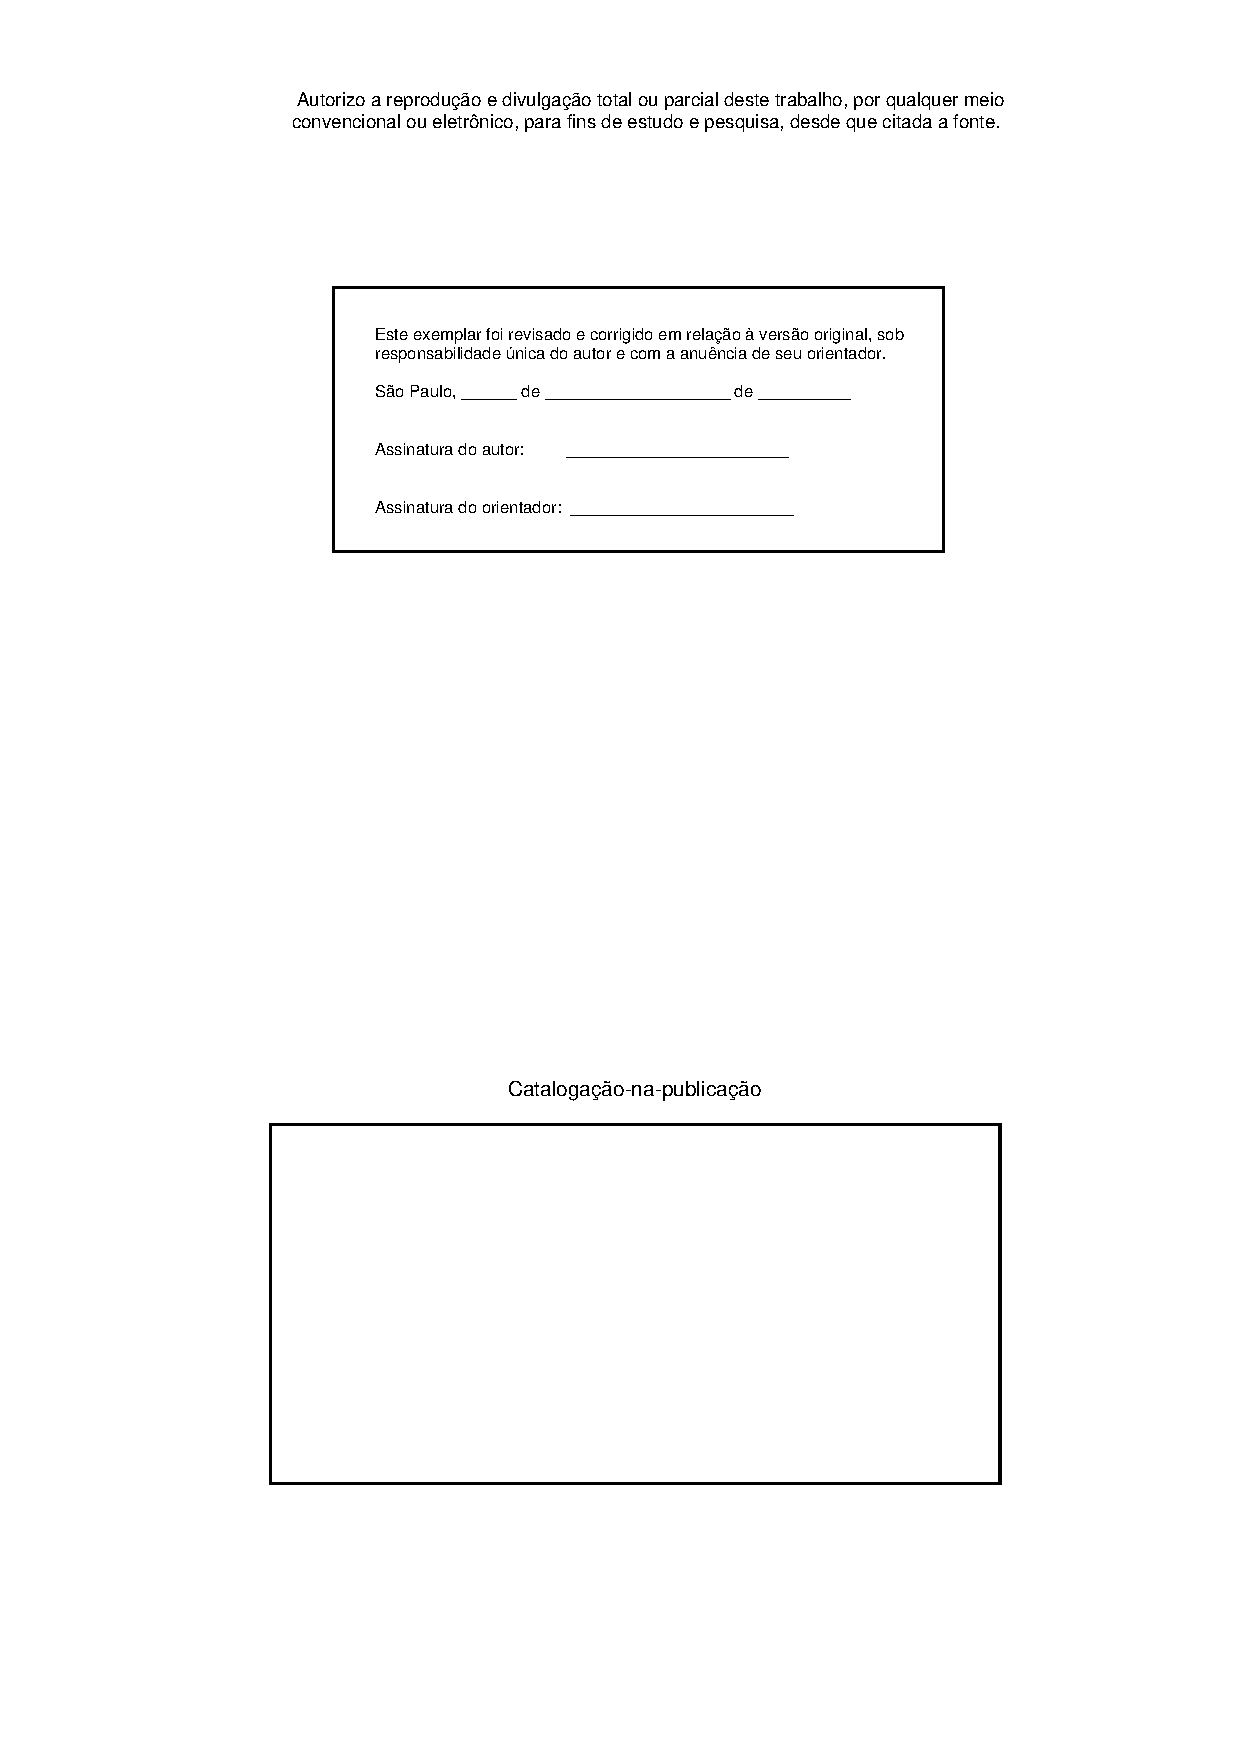
\includepdf[pages=1,scale=1,pagecommand={},linktodoc=true]{ficha.pdf}
% ========== Folha de assinaturas (opcional) ==========
%\begin{folhadeaprovacao}
%	\assinatura{Orientador}
%	\assinatura{Avaliador 1}
%	\assinatura{Avaliador 2}
%\end{folhadeaprovacao}


% ========== Dedicatória (opcional) ==========
\dedicatoria{Dedicatória}
\blindtext

% ========== Agradecimentos ==========
\begin{agradecimentos}

\blindtext

\end{agradecimentos}


% ========== Epígrafe (opcional) ==========
\epigrafe{%
	\emph{``Epígrafe''}
	\begin{flushright}
		\blindtext
	\end{flushright}
}


% ========== Resumo ==========
\begin{resumo}
\blindtext
%
\\[3\baselineskip]
%
\textbf{Palavras-Chave} --palavra1, palavra2, palavra3.
\end{resumo}

% ========== Abstract ==========
\begin{abstract}
\blindtext
%
\\[3\baselineskip]
%
\textbf{Keywords} -- key1,key2,key3.
\end{abstract}

% ========== Listas (opcional) ==========
\listadefiguras
\listadetabelas

% ========== Listas definidas pelo usuário (opcional) ==========
\begin{pretextualsection}{Lista de Siglas}

\noindent
ASP – \textit{American Society of Photogrametry} (Sociedade Americana de Fotogrametria)\\ \\


\end{pretextualsection}

% ========== Sumário ==========
\sumario

% ========== Elementos textuais =======

\chapter{Introdução}
\label{chapterIntroducao}
\blindtext
	
 \section{Considerações Iniciais}
	
	\blindtext
	
	\section{Justificativa}
	
	\blindtext
	
 \section{Objetivo}
	
	\blindtext
	
\chapter{Capitulo 1}
	
	\begin{figure}[H]
		\centering
		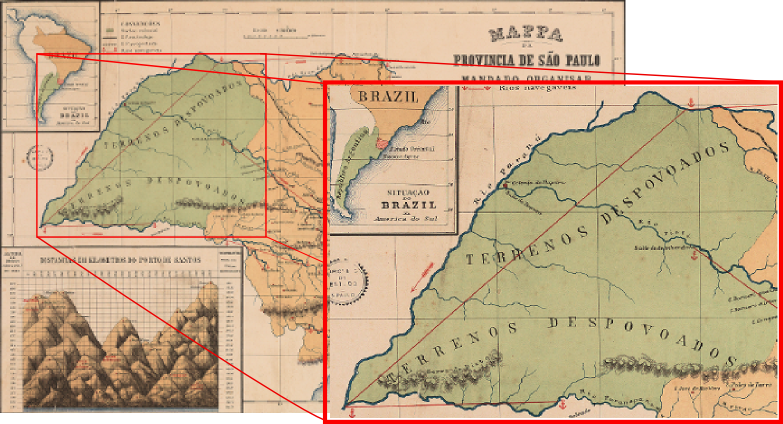
\includegraphics[width=0.9\linewidth]{provincia}
		\caption{Figura mapa 1} 
		Fonte: \citeonline{acervo}
		\label{fig:mapacgg}
	\end{figure}
\chapter{Conclusão}
\begin{citacaoLonga}
	\blindtext[5]			 
\end{citacaoLonga}
	A partir da equação \ref{eq1} pode-se calcular.
	
		\begin{equation}
		\begin{aligned}
		mf=c\sqrt{mc}
		\end{aligned}
		\label{eq1}
		\end{equation}
		
		
			\begin{table}[H]
    \centering
		\begin{tabular}{l|l}
			\hline
			\multicolumn{1}{c|}{\textbf{1:mc}} & \multicolumn{1}{c}{\textbf{1:mf}} \\ \hline
			1:500 & 1:3.500-1:5.000 \\ \hline
			1:1.000 & 1:5.100-1:8.000 \\ \hline
			1:2.500 & 1:8.500-1:13.000 \\ \hline
			1:5.000 & 1:12.100-1:18.000 \\ \hline
			1:10.000 & 1:17.000-1:26.000 \\ \hline
			1:25.000 & 1:28.000-1:42.000 \\ \hline
			1:50.000 & 1:40.000-1:60.000 \\ \hline
			1:100.000 & 1:60.000-1:90.000 \\ \hline
		\end{tabular}
		\caption{Módulo de escala da foto para diversas escalas de carta}
    Autor: \citeonline[p.5]{acervo}
		\label{tb:escalas_fotos}
	\end{table}
	


	
%\chapter{Capítulo com epígrafe}
%\capepigrafe[0.5\textwidth]{``Frase espirituosa de um autor famoso''}{Autor famoso}


% ========== Referências ==========
% --- IEEE ---
%	http://www.ctan.org/tex-archive/macros/latex/contrib/IEEEtran
%\bibliographystyle{IEEEbib}

% --- ABNT (requer ABNTeX 2) ---
%	http://www.ctan.org/tex-archive/macros/latex/contrib/abntex2
%\bibliographystyle{abntex2-num}


% ========== Apêndices (opcional) ==========
\apendice
\chapter{Apendice}
\label{apendicecggigg}
\blindtext

\begin{figure}[H]
	\centering
	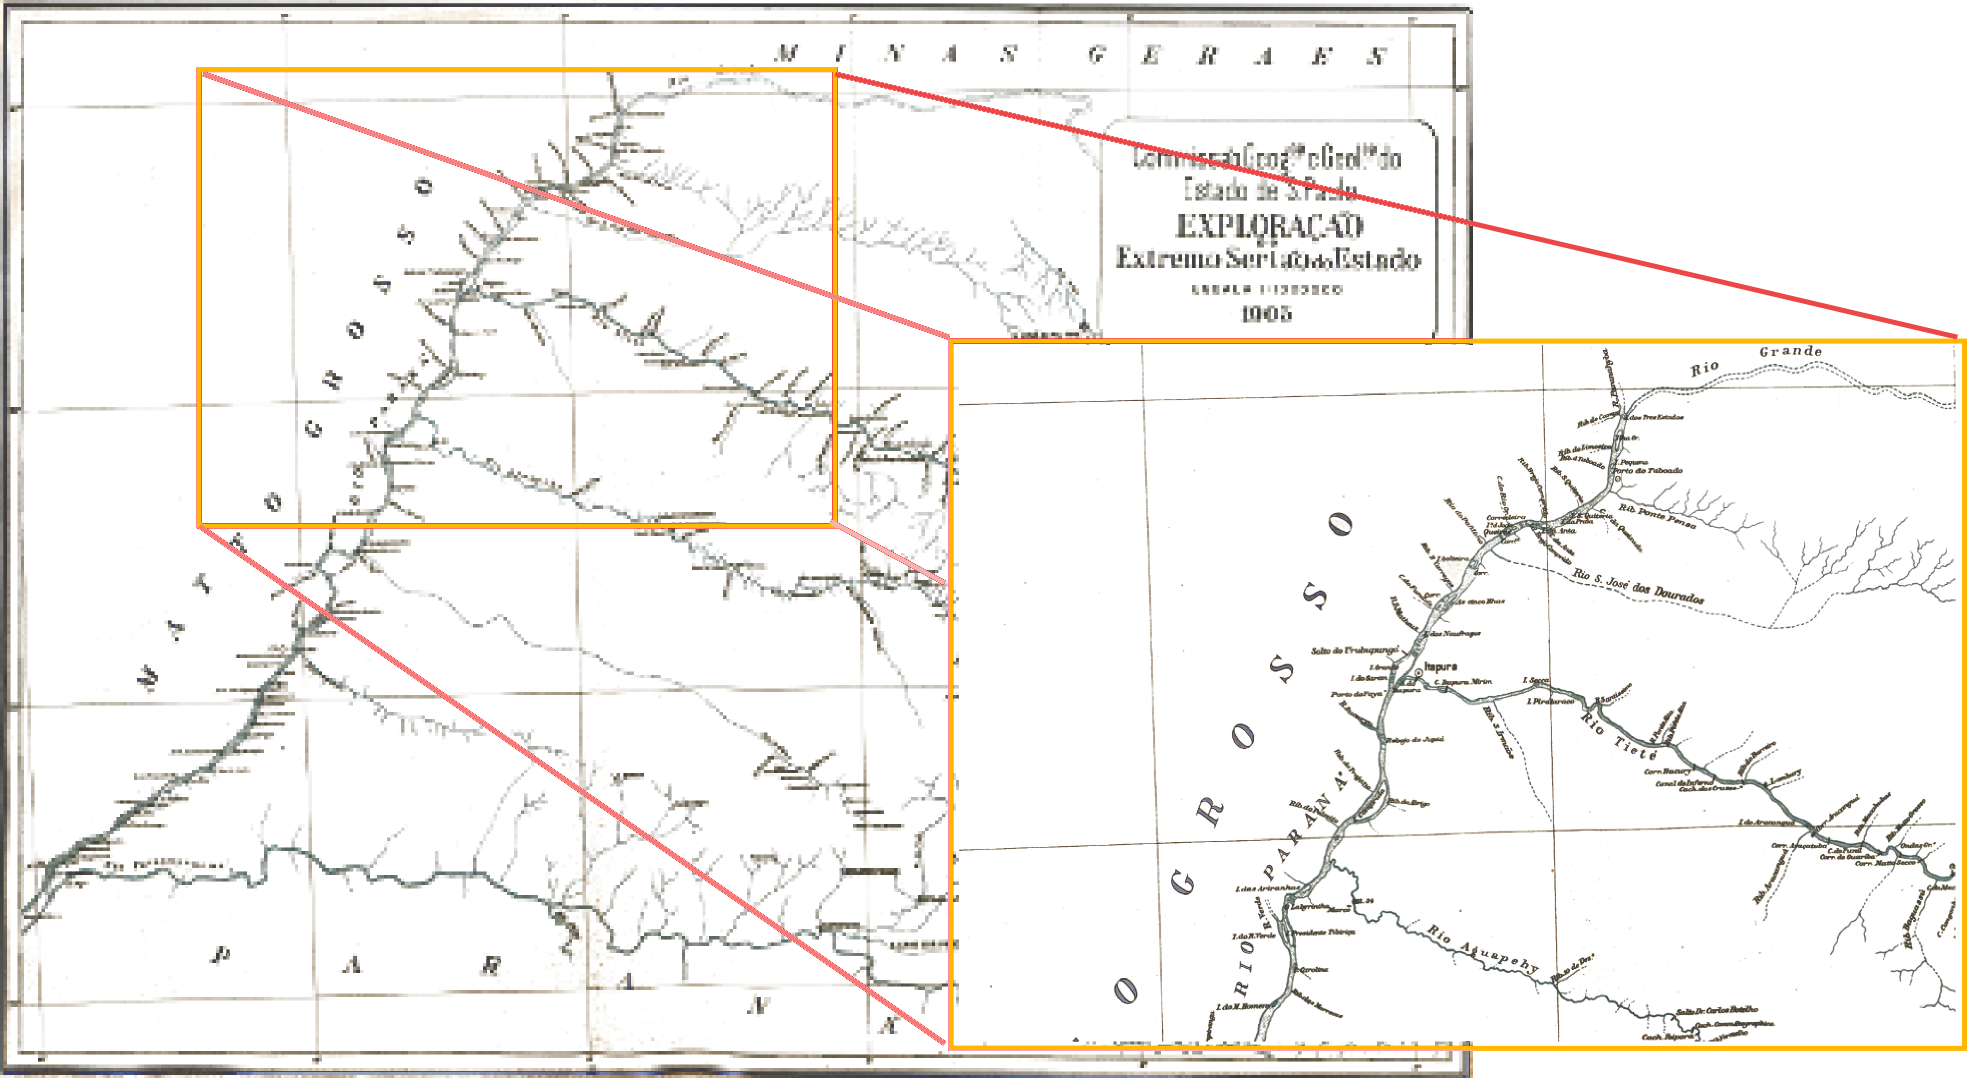
\includegraphics[width=0.92\linewidth]{cgg_oeste}
	\caption{Mapa 2} 
	Fonte: \citeonline{acervo}
	\label{fig:mapacgg2}
\end{figure}	

\newpage

\newpage
%\chapter{Beta}
% ========== Anexos (opcional) ==========
\anexo
%\chapter{Alpha}
\chapter{}
% Graphic for TeX using PGF
% Title: E:\mestrado\teste_mestrado\tabelas_esquemas\organizacao_38_69.dia
% Creator: Dia v0.97.2
% CreationDate: Wed Oct 11 23:43:39 2017
% For: Katia-PC
% \usepackage{tikz}
% The following commands are not supported in PSTricks at present
% We define them conditionally, so when they are implemented,
% this pgf file will use them.
\ifx\du\undefined
  \newlength{\du}
\fi
\begin{figure}[h]
	\centering
	\caption{\textbf{Organograma made by DIA}} \label{organizacao3869}
\setlength{\du}{15\unitlength}
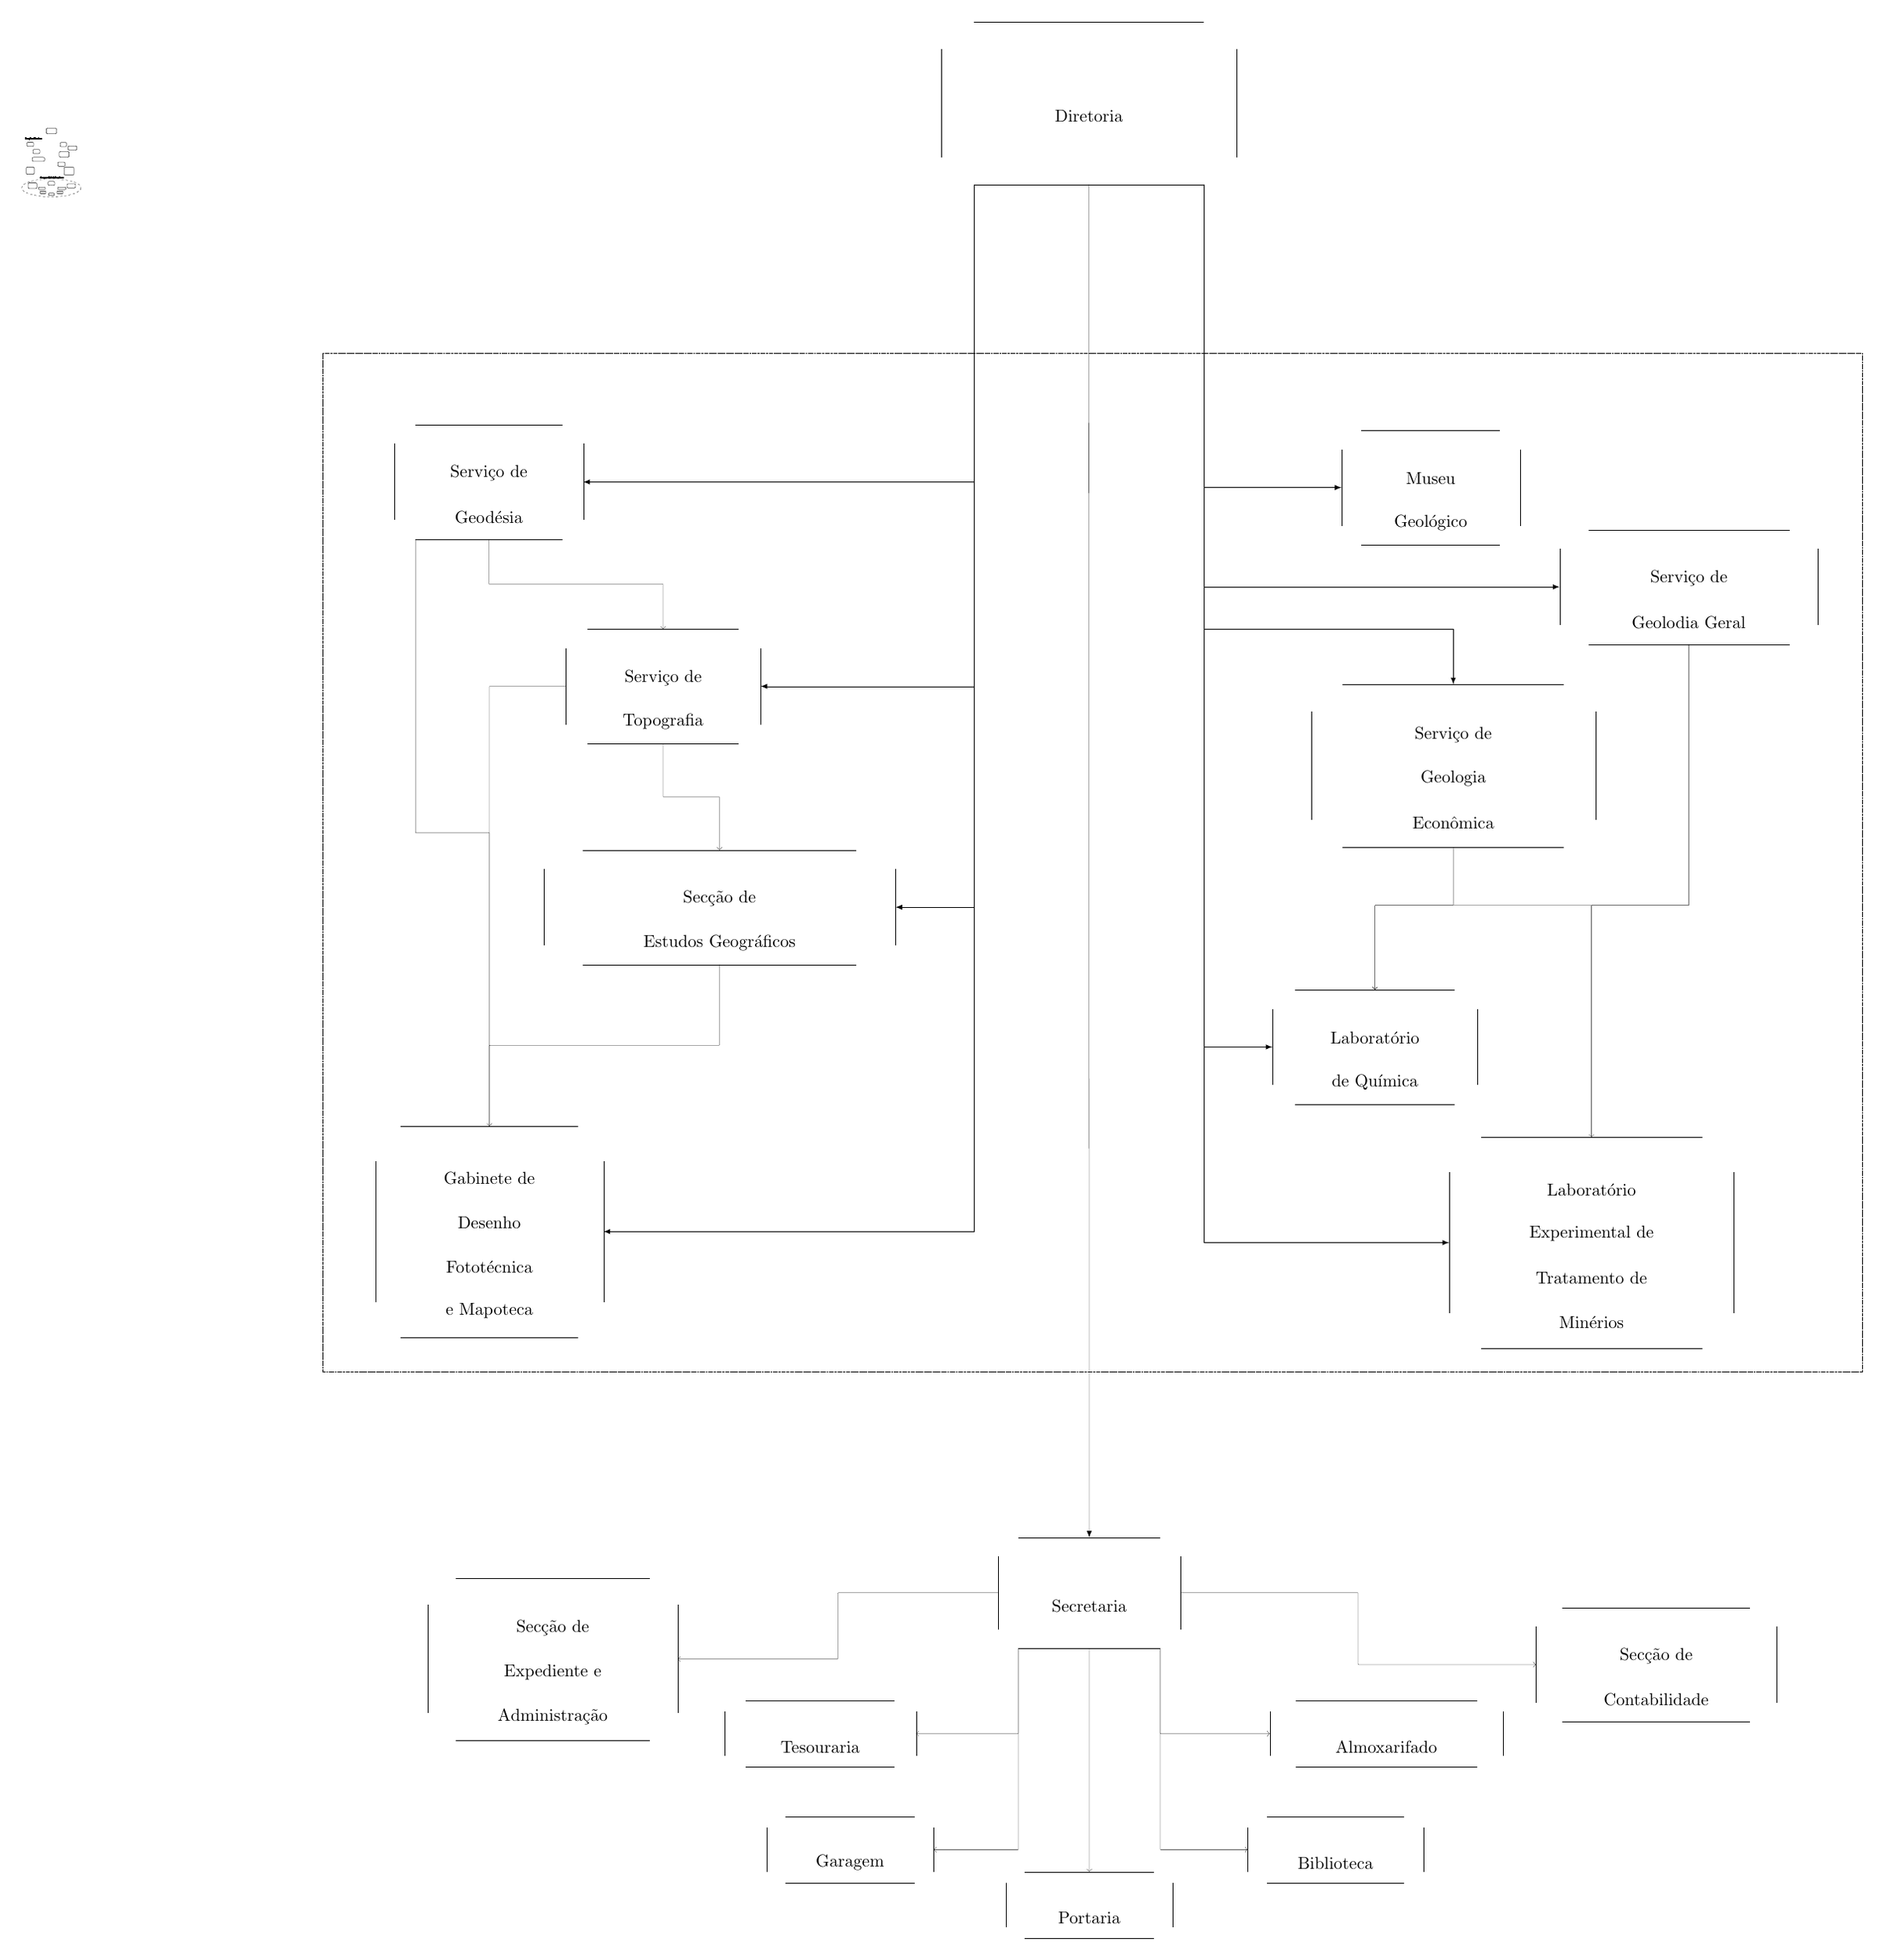
\begin{tikzpicture}[thick,scale=0.9, every node/.style={scale=0.8}]
\pgftransformxscale{1.000000}
\pgftransformyscale{-1.000000}
\definecolor{dialinecolor}{rgb}{0.000000, 0.000000, 0.000000}
\pgfsetstrokecolor{dialinecolor}
\definecolor{dialinecolor}{rgb}{1.000000, 1.000000, 1.000000}
\pgfsetfillcolor{dialinecolor}
\pgfsetlinewidth{0.100000\du}
\pgfsetdash{}{0pt}
\pgfsetdash{}{0pt}
\pgfsetbuttcap
\pgfsetmiterjoin
\pgfsetlinewidth{0.100000\du}
\pgfsetbuttcap
\pgfsetmiterjoin
\pgfsetdash{}{0pt}
\definecolor{dialinecolor}{rgb}{1.000000, 1.000000, 1.000000}
\pgfsetfillcolor{dialinecolor}
\pgfpathmoveto{\pgfpoint{17.394444\du}{-2.000000\du}}
\pgfpathcurveto{\pgfpoint{17.988889\du}{-2.000000\du}}{\pgfpoint{20.961111\du}{-2.000000\du}}{\pgfpoint{21.555556\du}{-2.000000\du}}
\pgfpathcurveto{\pgfpoint{22.150000\du}{-2.000000\du}}{\pgfpoint{22.150000\du}{-2.000000\du}}{\pgfpoint{22.150000\du}{-1.508333\du}}
\pgfpathcurveto{\pgfpoint{22.150000\du}{-1.016667\du}}{\pgfpoint{22.150000\du}{-0.033333\du}}{\pgfpoint{22.150000\du}{0.458333\du}}
\pgfpathcurveto{\pgfpoint{22.150000\du}{0.950000\du}}{\pgfpoint{22.150000\du}{0.950000\du}}{\pgfpoint{21.555556\du}{0.950000\du}}
\pgfpathcurveto{\pgfpoint{20.961111\du}{0.950000\du}}{\pgfpoint{17.988889\du}{0.950000\du}}{\pgfpoint{17.394444\du}{0.950000\du}}
\pgfpathcurveto{\pgfpoint{16.800000\du}{0.950000\du}}{\pgfpoint{16.800000\du}{0.950000\du}}{\pgfpoint{16.800000\du}{0.458333\du}}
\pgfpathcurveto{\pgfpoint{16.800000\du}{-0.033333\du}}{\pgfpoint{16.800000\du}{-1.016667\du}}{\pgfpoint{16.800000\du}{-1.508333\du}}
\pgfpathcurveto{\pgfpoint{16.800000\du}{-2.000000\du}}{\pgfpoint{16.800000\du}{-2.000000\du}}{\pgfpoint{17.394444\du}{-2.000000\du}}
\pgfusepath{fill}
\definecolor{dialinecolor}{rgb}{0.000000, 0.000000, 0.000000}
\pgfsetstrokecolor{dialinecolor}
\pgfpathmoveto{\pgfpoint{17.394444\du}{-2.000000\du}}
\pgfpathcurveto{\pgfpoint{17.988889\du}{-2.000000\du}}{\pgfpoint{20.961111\du}{-2.000000\du}}{\pgfpoint{21.555556\du}{-2.000000\du}}
\pgfpathcurveto{\pgfpoint{22.150000\du}{-2.000000\du}}{\pgfpoint{22.150000\du}{-2.000000\du}}{\pgfpoint{22.150000\du}{-1.508333\du}}
\pgfpathcurveto{\pgfpoint{22.150000\du}{-1.016667\du}}{\pgfpoint{22.150000\du}{-0.033333\du}}{\pgfpoint{22.150000\du}{0.458333\du}}
\pgfpathcurveto{\pgfpoint{22.150000\du}{0.950000\du}}{\pgfpoint{22.150000\du}{0.950000\du}}{\pgfpoint{21.555556\du}{0.950000\du}}
\pgfpathcurveto{\pgfpoint{20.961111\du}{0.950000\du}}{\pgfpoint{17.988889\du}{0.950000\du}}{\pgfpoint{17.394444\du}{0.950000\du}}
\pgfpathcurveto{\pgfpoint{16.800000\du}{0.950000\du}}{\pgfpoint{16.800000\du}{0.950000\du}}{\pgfpoint{16.800000\du}{0.458333\du}}
\pgfpathcurveto{\pgfpoint{16.800000\du}{-0.033333\du}}{\pgfpoint{16.800000\du}{-1.016667\du}}{\pgfpoint{16.800000\du}{-1.508333\du}}
\pgfpathcurveto{\pgfpoint{16.800000\du}{-2.000000\du}}{\pgfpoint{16.800000\du}{-2.000000\du}}{\pgfpoint{17.394444\du}{-2.000000\du}}
\pgfusepath{stroke}
\pgfsetlinewidth{0.010000\du}
\pgfsetbuttcap
\pgfsetmiterjoin
\pgfsetdash{}{0pt}
\definecolor{dialinecolor}{rgb}{0.000000, 0.000000, 0.000000}
\pgfsetstrokecolor{dialinecolor}
\pgfpathmoveto{\pgfpoint{17.394444\du}{-2.000000\du}}
\pgfpathcurveto{\pgfpoint{17.988889\du}{-2.000000\du}}{\pgfpoint{20.961111\du}{-2.000000\du}}{\pgfpoint{21.555556\du}{-2.000000\du}}
\pgfpathcurveto{\pgfpoint{22.150000\du}{-2.000000\du}}{\pgfpoint{22.150000\du}{-2.000000\du}}{\pgfpoint{22.150000\du}{-1.508333\du}}
\pgfpathcurveto{\pgfpoint{22.150000\du}{-1.016667\du}}{\pgfpoint{22.150000\du}{-0.033333\du}}{\pgfpoint{22.150000\du}{0.458333\du}}
\pgfpathcurveto{\pgfpoint{22.150000\du}{0.950000\du}}{\pgfpoint{22.150000\du}{0.950000\du}}{\pgfpoint{21.555556\du}{0.950000\du}}
\pgfpathcurveto{\pgfpoint{20.961111\du}{0.950000\du}}{\pgfpoint{17.988889\du}{0.950000\du}}{\pgfpoint{17.394444\du}{0.950000\du}}
\pgfpathcurveto{\pgfpoint{16.800000\du}{0.950000\du}}{\pgfpoint{16.800000\du}{0.950000\du}}{\pgfpoint{16.800000\du}{0.458333\du}}
\pgfpathcurveto{\pgfpoint{16.800000\du}{-0.033333\du}}{\pgfpoint{16.800000\du}{-1.016667\du}}{\pgfpoint{16.800000\du}{-1.508333\du}}
\pgfpathcurveto{\pgfpoint{16.800000\du}{-2.000000\du}}{\pgfpoint{16.800000\du}{-2.000000\du}}{\pgfpoint{17.394444\du}{-2.000000\du}}
\pgfusepath{stroke}
\pgfsetbuttcap
\pgfsetmiterjoin
\pgfsetdash{}{0pt}
\definecolor{dialinecolor}{rgb}{0.000000, 0.000000, 0.000000}
\pgfsetstrokecolor{dialinecolor}
\draw (17.394444\du,0.950000\du)--(21.555556\du,0.950000\du);
\pgfsetbuttcap
\pgfsetmiterjoin
\pgfsetdash{}{0pt}
\definecolor{dialinecolor}{rgb}{0.000000, 0.000000, 0.000000}
\pgfsetstrokecolor{dialinecolor}
\draw (22.150000\du,-1.508333\du)--(22.150000\du,0.458333\du);
\pgfsetbuttcap
\pgfsetmiterjoin
\pgfsetdash{}{0pt}
\definecolor{dialinecolor}{rgb}{0.000000, 0.000000, 0.000000}
\pgfsetstrokecolor{dialinecolor}
\draw (16.800000\du,-1.508333\du)--(16.800000\du,0.458333\du);
\pgfsetbuttcap
\pgfsetmiterjoin
\pgfsetdash{}{0pt}
\definecolor{dialinecolor}{rgb}{0.000000, 0.000000, 0.000000}
\pgfsetstrokecolor{dialinecolor}
\draw (17.394444\du,-2.000000\du)--(21.555556\du,-2.000000\du);
% setfont left to latex
\definecolor{dialinecolor}{rgb}{0.000000, 0.000000, 0.000000}
\pgfsetstrokecolor{dialinecolor}
\node at (19.475000\du,-0.285000\du){Diretoria};
\pgfsetlinewidth{0.100000\du}
\pgfsetdash{}{0pt}
\pgfsetdash{}{0pt}
\pgfsetbuttcap
\pgfsetmiterjoin
\pgfsetlinewidth{0.100000\du}
\pgfsetbuttcap
\pgfsetmiterjoin
\pgfsetdash{}{0pt}
\definecolor{dialinecolor}{rgb}{1.000000, 1.000000, 1.000000}
\pgfsetfillcolor{dialinecolor}
\pgfpathmoveto{\pgfpoint{10.392059\du}{9.000000\du}}
\pgfpathcurveto{\pgfpoint{10.784118\du}{9.000000\du}}{\pgfpoint{12.744412\du}{9.000000\du}}{\pgfpoint{13.136471\du}{9.000000\du}}
\pgfpathcurveto{\pgfpoint{13.528529\du}{9.000000\du}}{\pgfpoint{13.528529\du}{9.000000\du}}{\pgfpoint{13.528529\du}{9.345455\du}}
\pgfpathcurveto{\pgfpoint{13.528529\du}{9.690909\du}}{\pgfpoint{13.528529\du}{10.381818\du}}{\pgfpoint{13.528529\du}{10.727273\du}}
\pgfpathcurveto{\pgfpoint{13.528529\du}{11.072727\du}}{\pgfpoint{13.528529\du}{11.072727\du}}{\pgfpoint{13.136471\du}{11.072727\du}}
\pgfpathcurveto{\pgfpoint{12.744412\du}{11.072727\du}}{\pgfpoint{10.784118\du}{11.072727\du}}{\pgfpoint{10.392059\du}{11.072727\du}}
\pgfpathcurveto{\pgfpoint{10.000000\du}{11.072727\du}}{\pgfpoint{10.000000\du}{11.072727\du}}{\pgfpoint{10.000000\du}{10.727273\du}}
\pgfpathcurveto{\pgfpoint{10.000000\du}{10.381818\du}}{\pgfpoint{10.000000\du}{9.690909\du}}{\pgfpoint{10.000000\du}{9.345455\du}}
\pgfpathcurveto{\pgfpoint{10.000000\du}{9.000000\du}}{\pgfpoint{10.000000\du}{9.000000\du}}{\pgfpoint{10.392059\du}{9.000000\du}}
\pgfusepath{fill}
\definecolor{dialinecolor}{rgb}{0.000000, 0.000000, 0.000000}
\pgfsetstrokecolor{dialinecolor}
\pgfpathmoveto{\pgfpoint{10.392059\du}{9.000000\du}}
\pgfpathcurveto{\pgfpoint{10.784118\du}{9.000000\du}}{\pgfpoint{12.744412\du}{9.000000\du}}{\pgfpoint{13.136471\du}{9.000000\du}}
\pgfpathcurveto{\pgfpoint{13.528529\du}{9.000000\du}}{\pgfpoint{13.528529\du}{9.000000\du}}{\pgfpoint{13.528529\du}{9.345455\du}}
\pgfpathcurveto{\pgfpoint{13.528529\du}{9.690909\du}}{\pgfpoint{13.528529\du}{10.381818\du}}{\pgfpoint{13.528529\du}{10.727273\du}}
\pgfpathcurveto{\pgfpoint{13.528529\du}{11.072727\du}}{\pgfpoint{13.528529\du}{11.072727\du}}{\pgfpoint{13.136471\du}{11.072727\du}}
\pgfpathcurveto{\pgfpoint{12.744412\du}{11.072727\du}}{\pgfpoint{10.784118\du}{11.072727\du}}{\pgfpoint{10.392059\du}{11.072727\du}}
\pgfpathcurveto{\pgfpoint{10.000000\du}{11.072727\du}}{\pgfpoint{10.000000\du}{11.072727\du}}{\pgfpoint{10.000000\du}{10.727273\du}}
\pgfpathcurveto{\pgfpoint{10.000000\du}{10.381818\du}}{\pgfpoint{10.000000\du}{9.690909\du}}{\pgfpoint{10.000000\du}{9.345455\du}}
\pgfpathcurveto{\pgfpoint{10.000000\du}{9.000000\du}}{\pgfpoint{10.000000\du}{9.000000\du}}{\pgfpoint{10.392059\du}{9.000000\du}}
\pgfusepath{stroke}
\pgfsetlinewidth{0.010000\du}
\pgfsetbuttcap
\pgfsetmiterjoin
\pgfsetdash{}{0pt}
\definecolor{dialinecolor}{rgb}{0.000000, 0.000000, 0.000000}
\pgfsetstrokecolor{dialinecolor}
\pgfpathmoveto{\pgfpoint{10.392059\du}{9.000000\du}}
\pgfpathcurveto{\pgfpoint{10.784118\du}{9.000000\du}}{\pgfpoint{12.744412\du}{9.000000\du}}{\pgfpoint{13.136471\du}{9.000000\du}}
\pgfpathcurveto{\pgfpoint{13.528529\du}{9.000000\du}}{\pgfpoint{13.528529\du}{9.000000\du}}{\pgfpoint{13.528529\du}{9.345455\du}}
\pgfpathcurveto{\pgfpoint{13.528529\du}{9.690909\du}}{\pgfpoint{13.528529\du}{10.381818\du}}{\pgfpoint{13.528529\du}{10.727273\du}}
\pgfpathcurveto{\pgfpoint{13.528529\du}{11.072727\du}}{\pgfpoint{13.528529\du}{11.072727\du}}{\pgfpoint{13.136471\du}{11.072727\du}}
\pgfpathcurveto{\pgfpoint{12.744412\du}{11.072727\du}}{\pgfpoint{10.784118\du}{11.072727\du}}{\pgfpoint{10.392059\du}{11.072727\du}}
\pgfpathcurveto{\pgfpoint{10.000000\du}{11.072727\du}}{\pgfpoint{10.000000\du}{11.072727\du}}{\pgfpoint{10.000000\du}{10.727273\du}}
\pgfpathcurveto{\pgfpoint{10.000000\du}{10.381818\du}}{\pgfpoint{10.000000\du}{9.690909\du}}{\pgfpoint{10.000000\du}{9.345455\du}}
\pgfpathcurveto{\pgfpoint{10.000000\du}{9.000000\du}}{\pgfpoint{10.000000\du}{9.000000\du}}{\pgfpoint{10.392059\du}{9.000000\du}}
\pgfusepath{stroke}
\pgfsetbuttcap
\pgfsetmiterjoin
\pgfsetdash{}{0pt}
\definecolor{dialinecolor}{rgb}{0.000000, 0.000000, 0.000000}
\pgfsetstrokecolor{dialinecolor}
\draw (10.392059\du,11.072727\du)--(13.136471\du,11.072727\du);
\pgfsetbuttcap
\pgfsetmiterjoin
\pgfsetdash{}{0pt}
\definecolor{dialinecolor}{rgb}{0.000000, 0.000000, 0.000000}
\pgfsetstrokecolor{dialinecolor}
\draw (13.528529\du,9.345455\du)--(13.528529\du,10.727273\du);
\pgfsetbuttcap
\pgfsetmiterjoin
\pgfsetdash{}{0pt}
\definecolor{dialinecolor}{rgb}{0.000000, 0.000000, 0.000000}
\pgfsetstrokecolor{dialinecolor}
\draw (10.000000\du,9.345455\du)--(10.000000\du,10.727273\du);
\pgfsetbuttcap
\pgfsetmiterjoin
\pgfsetdash{}{0pt}
\definecolor{dialinecolor}{rgb}{0.000000, 0.000000, 0.000000}
\pgfsetstrokecolor{dialinecolor}
\draw (10.392059\du,9.000000\du)--(13.136471\du,9.000000\du);
% setfont left to latex
\definecolor{dialinecolor}{rgb}{0.000000, 0.000000, 0.000000}
\pgfsetstrokecolor{dialinecolor}
\node at (11.764265\du,9.876364\du){Serviço de};
% setfont left to latex
\definecolor{dialinecolor}{rgb}{0.000000, 0.000000, 0.000000}
\pgfsetstrokecolor{dialinecolor}
\node at (11.764265\du,10.676364\du){Topografia};
\pgfsetlinewidth{0.100000\du}
\pgfsetdash{}{0pt}
\pgfsetdash{}{0pt}
\pgfsetbuttcap
\pgfsetmiterjoin
\pgfsetlinewidth{0.100000\du}
\pgfsetbuttcap
\pgfsetmiterjoin
\pgfsetdash{}{0pt}
\definecolor{dialinecolor}{rgb}{1.000000, 1.000000, 1.000000}
\pgfsetfillcolor{dialinecolor}
\pgfpathmoveto{\pgfpoint{7.279706\du}{5.300000\du}}
\pgfpathcurveto{\pgfpoint{7.659412\du}{5.300000\du}}{\pgfpoint{9.557941\du}{5.300000\du}}{\pgfpoint{9.937647\du}{5.300000\du}}
\pgfpathcurveto{\pgfpoint{10.317353\du}{5.300000\du}}{\pgfpoint{10.317353\du}{5.300000\du}}{\pgfpoint{10.317353\du}{5.645455\du}}
\pgfpathcurveto{\pgfpoint{10.317353\du}{5.990909\du}}{\pgfpoint{10.317353\du}{6.681818\du}}{\pgfpoint{10.317353\du}{7.027273\du}}
\pgfpathcurveto{\pgfpoint{10.317353\du}{7.372727\du}}{\pgfpoint{10.317353\du}{7.372727\du}}{\pgfpoint{9.937647\du}{7.372727\du}}
\pgfpathcurveto{\pgfpoint{9.557941\du}{7.372727\du}}{\pgfpoint{7.659412\du}{7.372727\du}}{\pgfpoint{7.279706\du}{7.372727\du}}
\pgfpathcurveto{\pgfpoint{6.900000\du}{7.372727\du}}{\pgfpoint{6.900000\du}{7.372727\du}}{\pgfpoint{6.900000\du}{7.027273\du}}
\pgfpathcurveto{\pgfpoint{6.900000\du}{6.681818\du}}{\pgfpoint{6.900000\du}{5.990909\du}}{\pgfpoint{6.900000\du}{5.645455\du}}
\pgfpathcurveto{\pgfpoint{6.900000\du}{5.300000\du}}{\pgfpoint{6.900000\du}{5.300000\du}}{\pgfpoint{7.279706\du}{5.300000\du}}
\pgfusepath{fill}
\definecolor{dialinecolor}{rgb}{0.000000, 0.000000, 0.000000}
\pgfsetstrokecolor{dialinecolor}
\pgfpathmoveto{\pgfpoint{7.279706\du}{5.300000\du}}
\pgfpathcurveto{\pgfpoint{7.659412\du}{5.300000\du}}{\pgfpoint{9.557941\du}{5.300000\du}}{\pgfpoint{9.937647\du}{5.300000\du}}
\pgfpathcurveto{\pgfpoint{10.317353\du}{5.300000\du}}{\pgfpoint{10.317353\du}{5.300000\du}}{\pgfpoint{10.317353\du}{5.645455\du}}
\pgfpathcurveto{\pgfpoint{10.317353\du}{5.990909\du}}{\pgfpoint{10.317353\du}{6.681818\du}}{\pgfpoint{10.317353\du}{7.027273\du}}
\pgfpathcurveto{\pgfpoint{10.317353\du}{7.372727\du}}{\pgfpoint{10.317353\du}{7.372727\du}}{\pgfpoint{9.937647\du}{7.372727\du}}
\pgfpathcurveto{\pgfpoint{9.557941\du}{7.372727\du}}{\pgfpoint{7.659412\du}{7.372727\du}}{\pgfpoint{7.279706\du}{7.372727\du}}
\pgfpathcurveto{\pgfpoint{6.900000\du}{7.372727\du}}{\pgfpoint{6.900000\du}{7.372727\du}}{\pgfpoint{6.900000\du}{7.027273\du}}
\pgfpathcurveto{\pgfpoint{6.900000\du}{6.681818\du}}{\pgfpoint{6.900000\du}{5.990909\du}}{\pgfpoint{6.900000\du}{5.645455\du}}
\pgfpathcurveto{\pgfpoint{6.900000\du}{5.300000\du}}{\pgfpoint{6.900000\du}{5.300000\du}}{\pgfpoint{7.279706\du}{5.300000\du}}
\pgfusepath{stroke}
\pgfsetlinewidth{0.010000\du}
\pgfsetbuttcap
\pgfsetmiterjoin
\pgfsetdash{}{0pt}
\definecolor{dialinecolor}{rgb}{0.000000, 0.000000, 0.000000}
\pgfsetstrokecolor{dialinecolor}
\pgfpathmoveto{\pgfpoint{7.279706\du}{5.300000\du}}
\pgfpathcurveto{\pgfpoint{7.659412\du}{5.300000\du}}{\pgfpoint{9.557941\du}{5.300000\du}}{\pgfpoint{9.937647\du}{5.300000\du}}
\pgfpathcurveto{\pgfpoint{10.317353\du}{5.300000\du}}{\pgfpoint{10.317353\du}{5.300000\du}}{\pgfpoint{10.317353\du}{5.645455\du}}
\pgfpathcurveto{\pgfpoint{10.317353\du}{5.990909\du}}{\pgfpoint{10.317353\du}{6.681818\du}}{\pgfpoint{10.317353\du}{7.027273\du}}
\pgfpathcurveto{\pgfpoint{10.317353\du}{7.372727\du}}{\pgfpoint{10.317353\du}{7.372727\du}}{\pgfpoint{9.937647\du}{7.372727\du}}
\pgfpathcurveto{\pgfpoint{9.557941\du}{7.372727\du}}{\pgfpoint{7.659412\du}{7.372727\du}}{\pgfpoint{7.279706\du}{7.372727\du}}
\pgfpathcurveto{\pgfpoint{6.900000\du}{7.372727\du}}{\pgfpoint{6.900000\du}{7.372727\du}}{\pgfpoint{6.900000\du}{7.027273\du}}
\pgfpathcurveto{\pgfpoint{6.900000\du}{6.681818\du}}{\pgfpoint{6.900000\du}{5.990909\du}}{\pgfpoint{6.900000\du}{5.645455\du}}
\pgfpathcurveto{\pgfpoint{6.900000\du}{5.300000\du}}{\pgfpoint{6.900000\du}{5.300000\du}}{\pgfpoint{7.279706\du}{5.300000\du}}
\pgfusepath{stroke}
\pgfsetbuttcap
\pgfsetmiterjoin
\pgfsetdash{}{0pt}
\definecolor{dialinecolor}{rgb}{0.000000, 0.000000, 0.000000}
\pgfsetstrokecolor{dialinecolor}
\draw (7.279706\du,7.372727\du)--(9.937647\du,7.372727\du);
\pgfsetbuttcap
\pgfsetmiterjoin
\pgfsetdash{}{0pt}
\definecolor{dialinecolor}{rgb}{0.000000, 0.000000, 0.000000}
\pgfsetstrokecolor{dialinecolor}
\draw (10.317353\du,5.645455\du)--(10.317353\du,7.027273\du);
\pgfsetbuttcap
\pgfsetmiterjoin
\pgfsetdash{}{0pt}
\definecolor{dialinecolor}{rgb}{0.000000, 0.000000, 0.000000}
\pgfsetstrokecolor{dialinecolor}
\draw (6.900000\du,5.645455\du)--(6.900000\du,7.027273\du);
\pgfsetbuttcap
\pgfsetmiterjoin
\pgfsetdash{}{0pt}
\definecolor{dialinecolor}{rgb}{0.000000, 0.000000, 0.000000}
\pgfsetstrokecolor{dialinecolor}
\draw (7.279706\du,5.300000\du)--(9.937647\du,5.300000\du);
% setfont left to latex
\definecolor{dialinecolor}{rgb}{0.000000, 0.000000, 0.000000}
\pgfsetstrokecolor{dialinecolor}
\node at (8.608676\du,6.176364\du){Serviço de};
% setfont left to latex
\definecolor{dialinecolor}{rgb}{0.000000, 0.000000, 0.000000}
\pgfsetstrokecolor{dialinecolor}
\node at (8.608676\du,6.976364\du){Geodésia};
\pgfsetlinewidth{0.100000\du}
\pgfsetdash{}{0pt}
\pgfsetdash{}{0pt}
\pgfsetbuttcap
\pgfsetmiterjoin
\pgfsetlinewidth{0.100000\du}
\pgfsetbuttcap
\pgfsetmiterjoin
\pgfsetdash{}{0pt}
\definecolor{dialinecolor}{rgb}{1.000000, 1.000000, 1.000000}
\pgfsetfillcolor{dialinecolor}
\pgfpathmoveto{\pgfpoint{28.520294\du}{7.200000\du}}
\pgfpathcurveto{\pgfpoint{29.040588\du}{7.200000\du}}{\pgfpoint{31.642059\du}{7.200000\du}}{\pgfpoint{32.162353\du}{7.200000\du}}
\pgfpathcurveto{\pgfpoint{32.682647\du}{7.200000\du}}{\pgfpoint{32.682647\du}{7.200000\du}}{\pgfpoint{32.682647\du}{7.545455\du}}
\pgfpathcurveto{\pgfpoint{32.682647\du}{7.890909\du}}{\pgfpoint{32.682647\du}{8.581818\du}}{\pgfpoint{32.682647\du}{8.927273\du}}
\pgfpathcurveto{\pgfpoint{32.682647\du}{9.272727\du}}{\pgfpoint{32.682647\du}{9.272727\du}}{\pgfpoint{32.162353\du}{9.272727\du}}
\pgfpathcurveto{\pgfpoint{31.642059\du}{9.272727\du}}{\pgfpoint{29.040588\du}{9.272727\du}}{\pgfpoint{28.520294\du}{9.272727\du}}
\pgfpathcurveto{\pgfpoint{28.000000\du}{9.272727\du}}{\pgfpoint{28.000000\du}{9.272727\du}}{\pgfpoint{28.000000\du}{8.927273\du}}
\pgfpathcurveto{\pgfpoint{28.000000\du}{8.581818\du}}{\pgfpoint{28.000000\du}{7.890909\du}}{\pgfpoint{28.000000\du}{7.545455\du}}
\pgfpathcurveto{\pgfpoint{28.000000\du}{7.200000\du}}{\pgfpoint{28.000000\du}{7.200000\du}}{\pgfpoint{28.520294\du}{7.200000\du}}
\pgfusepath{fill}
\definecolor{dialinecolor}{rgb}{0.000000, 0.000000, 0.000000}
\pgfsetstrokecolor{dialinecolor}
\pgfpathmoveto{\pgfpoint{28.520294\du}{7.200000\du}}
\pgfpathcurveto{\pgfpoint{29.040588\du}{7.200000\du}}{\pgfpoint{31.642059\du}{7.200000\du}}{\pgfpoint{32.162353\du}{7.200000\du}}
\pgfpathcurveto{\pgfpoint{32.682647\du}{7.200000\du}}{\pgfpoint{32.682647\du}{7.200000\du}}{\pgfpoint{32.682647\du}{7.545455\du}}
\pgfpathcurveto{\pgfpoint{32.682647\du}{7.890909\du}}{\pgfpoint{32.682647\du}{8.581818\du}}{\pgfpoint{32.682647\du}{8.927273\du}}
\pgfpathcurveto{\pgfpoint{32.682647\du}{9.272727\du}}{\pgfpoint{32.682647\du}{9.272727\du}}{\pgfpoint{32.162353\du}{9.272727\du}}
\pgfpathcurveto{\pgfpoint{31.642059\du}{9.272727\du}}{\pgfpoint{29.040588\du}{9.272727\du}}{\pgfpoint{28.520294\du}{9.272727\du}}
\pgfpathcurveto{\pgfpoint{28.000000\du}{9.272727\du}}{\pgfpoint{28.000000\du}{9.272727\du}}{\pgfpoint{28.000000\du}{8.927273\du}}
\pgfpathcurveto{\pgfpoint{28.000000\du}{8.581818\du}}{\pgfpoint{28.000000\du}{7.890909\du}}{\pgfpoint{28.000000\du}{7.545455\du}}
\pgfpathcurveto{\pgfpoint{28.000000\du}{7.200000\du}}{\pgfpoint{28.000000\du}{7.200000\du}}{\pgfpoint{28.520294\du}{7.200000\du}}
\pgfusepath{stroke}
\pgfsetlinewidth{0.010000\du}
\pgfsetbuttcap
\pgfsetmiterjoin
\pgfsetdash{}{0pt}
\definecolor{dialinecolor}{rgb}{0.000000, 0.000000, 0.000000}
\pgfsetstrokecolor{dialinecolor}
\pgfpathmoveto{\pgfpoint{28.520294\du}{7.200000\du}}
\pgfpathcurveto{\pgfpoint{29.040588\du}{7.200000\du}}{\pgfpoint{31.642059\du}{7.200000\du}}{\pgfpoint{32.162353\du}{7.200000\du}}
\pgfpathcurveto{\pgfpoint{32.682647\du}{7.200000\du}}{\pgfpoint{32.682647\du}{7.200000\du}}{\pgfpoint{32.682647\du}{7.545455\du}}
\pgfpathcurveto{\pgfpoint{32.682647\du}{7.890909\du}}{\pgfpoint{32.682647\du}{8.581818\du}}{\pgfpoint{32.682647\du}{8.927273\du}}
\pgfpathcurveto{\pgfpoint{32.682647\du}{9.272727\du}}{\pgfpoint{32.682647\du}{9.272727\du}}{\pgfpoint{32.162353\du}{9.272727\du}}
\pgfpathcurveto{\pgfpoint{31.642059\du}{9.272727\du}}{\pgfpoint{29.040588\du}{9.272727\du}}{\pgfpoint{28.520294\du}{9.272727\du}}
\pgfpathcurveto{\pgfpoint{28.000000\du}{9.272727\du}}{\pgfpoint{28.000000\du}{9.272727\du}}{\pgfpoint{28.000000\du}{8.927273\du}}
\pgfpathcurveto{\pgfpoint{28.000000\du}{8.581818\du}}{\pgfpoint{28.000000\du}{7.890909\du}}{\pgfpoint{28.000000\du}{7.545455\du}}
\pgfpathcurveto{\pgfpoint{28.000000\du}{7.200000\du}}{\pgfpoint{28.000000\du}{7.200000\du}}{\pgfpoint{28.520294\du}{7.200000\du}}
\pgfusepath{stroke}
\pgfsetbuttcap
\pgfsetmiterjoin
\pgfsetdash{}{0pt}
\definecolor{dialinecolor}{rgb}{0.000000, 0.000000, 0.000000}
\pgfsetstrokecolor{dialinecolor}
\draw (28.520294\du,9.272727\du)--(32.162353\du,9.272727\du);
\pgfsetbuttcap
\pgfsetmiterjoin
\pgfsetdash{}{0pt}
\definecolor{dialinecolor}{rgb}{0.000000, 0.000000, 0.000000}
\pgfsetstrokecolor{dialinecolor}
\draw (32.682647\du,7.545455\du)--(32.682647\du,8.927273\du);
\pgfsetbuttcap
\pgfsetmiterjoin
\pgfsetdash{}{0pt}
\definecolor{dialinecolor}{rgb}{0.000000, 0.000000, 0.000000}
\pgfsetstrokecolor{dialinecolor}
\draw (28.000000\du,7.545455\du)--(28.000000\du,8.927273\du);
\pgfsetbuttcap
\pgfsetmiterjoin
\pgfsetdash{}{0pt}
\definecolor{dialinecolor}{rgb}{0.000000, 0.000000, 0.000000}
\pgfsetstrokecolor{dialinecolor}
\draw (28.520294\du,7.200000\du)--(32.162353\du,7.200000\du);
% setfont left to latex
\definecolor{dialinecolor}{rgb}{0.000000, 0.000000, 0.000000}
\pgfsetstrokecolor{dialinecolor}
\node at (30.341324\du,8.076364\du){Serviço de};
% setfont left to latex
\definecolor{dialinecolor}{rgb}{0.000000, 0.000000, 0.000000}
\pgfsetstrokecolor{dialinecolor}
\node at (30.341324\du,8.876364\du){Geolodia Geral};
\pgfsetlinewidth{0.100000\du}
\pgfsetdash{}{0pt}
\pgfsetdash{}{0pt}
\pgfsetbuttcap
\pgfsetmiterjoin
\pgfsetlinewidth{0.100000\du}
\pgfsetbuttcap
\pgfsetmiterjoin
\pgfsetdash{}{0pt}
\definecolor{dialinecolor}{rgb}{1.000000, 1.000000, 1.000000}
\pgfsetfillcolor{dialinecolor}
\pgfpathmoveto{\pgfpoint{24.072222\du}{10.000000\du}}
\pgfpathcurveto{\pgfpoint{24.644444\du}{10.000000\du}}{\pgfpoint{27.505556\du}{10.000000\du}}{\pgfpoint{28.077778\du}{10.000000\du}}
\pgfpathcurveto{\pgfpoint{28.650000\du}{10.000000\du}}{\pgfpoint{28.650000\du}{10.000000\du}}{\pgfpoint{28.650000\du}{10.490909\du}}
\pgfpathcurveto{\pgfpoint{28.650000\du}{10.981818\du}}{\pgfpoint{28.650000\du}{11.963636\du}}{\pgfpoint{28.650000\du}{12.454545\du}}
\pgfpathcurveto{\pgfpoint{28.650000\du}{12.945455\du}}{\pgfpoint{28.650000\du}{12.945455\du}}{\pgfpoint{28.077778\du}{12.945455\du}}
\pgfpathcurveto{\pgfpoint{27.505556\du}{12.945455\du}}{\pgfpoint{24.644444\du}{12.945455\du}}{\pgfpoint{24.072222\du}{12.945455\du}}
\pgfpathcurveto{\pgfpoint{23.500000\du}{12.945455\du}}{\pgfpoint{23.500000\du}{12.945455\du}}{\pgfpoint{23.500000\du}{12.454545\du}}
\pgfpathcurveto{\pgfpoint{23.500000\du}{11.963636\du}}{\pgfpoint{23.500000\du}{10.981818\du}}{\pgfpoint{23.500000\du}{10.490909\du}}
\pgfpathcurveto{\pgfpoint{23.500000\du}{10.000000\du}}{\pgfpoint{23.500000\du}{10.000000\du}}{\pgfpoint{24.072222\du}{10.000000\du}}
\pgfusepath{fill}
\definecolor{dialinecolor}{rgb}{0.000000, 0.000000, 0.000000}
\pgfsetstrokecolor{dialinecolor}
\pgfpathmoveto{\pgfpoint{24.072222\du}{10.000000\du}}
\pgfpathcurveto{\pgfpoint{24.644444\du}{10.000000\du}}{\pgfpoint{27.505556\du}{10.000000\du}}{\pgfpoint{28.077778\du}{10.000000\du}}
\pgfpathcurveto{\pgfpoint{28.650000\du}{10.000000\du}}{\pgfpoint{28.650000\du}{10.000000\du}}{\pgfpoint{28.650000\du}{10.490909\du}}
\pgfpathcurveto{\pgfpoint{28.650000\du}{10.981818\du}}{\pgfpoint{28.650000\du}{11.963636\du}}{\pgfpoint{28.650000\du}{12.454545\du}}
\pgfpathcurveto{\pgfpoint{28.650000\du}{12.945455\du}}{\pgfpoint{28.650000\du}{12.945455\du}}{\pgfpoint{28.077778\du}{12.945455\du}}
\pgfpathcurveto{\pgfpoint{27.505556\du}{12.945455\du}}{\pgfpoint{24.644444\du}{12.945455\du}}{\pgfpoint{24.072222\du}{12.945455\du}}
\pgfpathcurveto{\pgfpoint{23.500000\du}{12.945455\du}}{\pgfpoint{23.500000\du}{12.945455\du}}{\pgfpoint{23.500000\du}{12.454545\du}}
\pgfpathcurveto{\pgfpoint{23.500000\du}{11.963636\du}}{\pgfpoint{23.500000\du}{10.981818\du}}{\pgfpoint{23.500000\du}{10.490909\du}}
\pgfpathcurveto{\pgfpoint{23.500000\du}{10.000000\du}}{\pgfpoint{23.500000\du}{10.000000\du}}{\pgfpoint{24.072222\du}{10.000000\du}}
\pgfusepath{stroke}
\pgfsetlinewidth{0.010000\du}
\pgfsetbuttcap
\pgfsetmiterjoin
\pgfsetdash{}{0pt}
\definecolor{dialinecolor}{rgb}{0.000000, 0.000000, 0.000000}
\pgfsetstrokecolor{dialinecolor}
\pgfpathmoveto{\pgfpoint{24.072222\du}{10.000000\du}}
\pgfpathcurveto{\pgfpoint{24.644444\du}{10.000000\du}}{\pgfpoint{27.505556\du}{10.000000\du}}{\pgfpoint{28.077778\du}{10.000000\du}}
\pgfpathcurveto{\pgfpoint{28.650000\du}{10.000000\du}}{\pgfpoint{28.650000\du}{10.000000\du}}{\pgfpoint{28.650000\du}{10.490909\du}}
\pgfpathcurveto{\pgfpoint{28.650000\du}{10.981818\du}}{\pgfpoint{28.650000\du}{11.963636\du}}{\pgfpoint{28.650000\du}{12.454545\du}}
\pgfpathcurveto{\pgfpoint{28.650000\du}{12.945455\du}}{\pgfpoint{28.650000\du}{12.945455\du}}{\pgfpoint{28.077778\du}{12.945455\du}}
\pgfpathcurveto{\pgfpoint{27.505556\du}{12.945455\du}}{\pgfpoint{24.644444\du}{12.945455\du}}{\pgfpoint{24.072222\du}{12.945455\du}}
\pgfpathcurveto{\pgfpoint{23.500000\du}{12.945455\du}}{\pgfpoint{23.500000\du}{12.945455\du}}{\pgfpoint{23.500000\du}{12.454545\du}}
\pgfpathcurveto{\pgfpoint{23.500000\du}{11.963636\du}}{\pgfpoint{23.500000\du}{10.981818\du}}{\pgfpoint{23.500000\du}{10.490909\du}}
\pgfpathcurveto{\pgfpoint{23.500000\du}{10.000000\du}}{\pgfpoint{23.500000\du}{10.000000\du}}{\pgfpoint{24.072222\du}{10.000000\du}}
\pgfusepath{stroke}
\pgfsetbuttcap
\pgfsetmiterjoin
\pgfsetdash{}{0pt}
\definecolor{dialinecolor}{rgb}{0.000000, 0.000000, 0.000000}
\pgfsetstrokecolor{dialinecolor}
\draw (24.072222\du,12.945455\du)--(28.077778\du,12.945455\du);
\pgfsetbuttcap
\pgfsetmiterjoin
\pgfsetdash{}{0pt}
\definecolor{dialinecolor}{rgb}{0.000000, 0.000000, 0.000000}
\pgfsetstrokecolor{dialinecolor}
\draw (28.650000\du,10.490909\du)--(28.650000\du,12.454545\du);
\pgfsetbuttcap
\pgfsetmiterjoin
\pgfsetdash{}{0pt}
\definecolor{dialinecolor}{rgb}{0.000000, 0.000000, 0.000000}
\pgfsetstrokecolor{dialinecolor}
\draw (23.500000\du,10.490909\du)--(23.500000\du,12.454545\du);
\pgfsetbuttcap
\pgfsetmiterjoin
\pgfsetdash{}{0pt}
\definecolor{dialinecolor}{rgb}{0.000000, 0.000000, 0.000000}
\pgfsetstrokecolor{dialinecolor}
\draw (24.072222\du,10.000000\du)--(28.077778\du,10.000000\du);
% setfont left to latex
\definecolor{dialinecolor}{rgb}{0.000000, 0.000000, 0.000000}
\pgfsetstrokecolor{dialinecolor}
\node at (26.075000\du,10.912727\du){Serviço de};
% setfont left to latex
\definecolor{dialinecolor}{rgb}{0.000000, 0.000000, 0.000000}
\pgfsetstrokecolor{dialinecolor}
\node at (26.075000\du,11.712727\du){Geologia};
% setfont left to latex
\definecolor{dialinecolor}{rgb}{0.000000, 0.000000, 0.000000}
\pgfsetstrokecolor{dialinecolor}
\node at (26.075000\du,12.512727\du){Econômica};
\pgfsetlinewidth{0.100000\du}
\pgfsetdash{}{0pt}
\pgfsetdash{}{0pt}
\pgfsetbuttcap
\pgfsetmiterjoin
\pgfsetlinewidth{0.100000\du}
\pgfsetbuttcap
\pgfsetmiterjoin
\pgfsetdash{}{0pt}
\definecolor{dialinecolor}{rgb}{1.000000, 1.000000, 1.000000}
\pgfsetfillcolor{dialinecolor}
\pgfpathmoveto{\pgfpoint{26.572941\du}{18.200000\du}}
\pgfpathcurveto{\pgfpoint{27.145882\du}{18.200000\du}}{\pgfpoint{30.010588\du}{18.200000\du}}{\pgfpoint{30.583529\du}{18.200000\du}}
\pgfpathcurveto{\pgfpoint{31.156471\du}{18.200000\du}}{\pgfpoint{31.156471\du}{18.200000\du}}{\pgfpoint{31.156471\du}{18.836364\du}}
\pgfpathcurveto{\pgfpoint{31.156471\du}{19.472727\du}}{\pgfpoint{31.156471\du}{20.745455\du}}{\pgfpoint{31.156471\du}{21.381818\du}}
\pgfpathcurveto{\pgfpoint{31.156471\du}{22.018182\du}}{\pgfpoint{31.156471\du}{22.018182\du}}{\pgfpoint{30.583529\du}{22.018182\du}}
\pgfpathcurveto{\pgfpoint{30.010588\du}{22.018182\du}}{\pgfpoint{27.145882\du}{22.018182\du}}{\pgfpoint{26.572941\du}{22.018182\du}}
\pgfpathcurveto{\pgfpoint{26.000000\du}{22.018182\du}}{\pgfpoint{26.000000\du}{22.018182\du}}{\pgfpoint{26.000000\du}{21.381818\du}}
\pgfpathcurveto{\pgfpoint{26.000000\du}{20.745455\du}}{\pgfpoint{26.000000\du}{19.472727\du}}{\pgfpoint{26.000000\du}{18.836364\du}}
\pgfpathcurveto{\pgfpoint{26.000000\du}{18.200000\du}}{\pgfpoint{26.000000\du}{18.200000\du}}{\pgfpoint{26.572941\du}{18.200000\du}}
\pgfusepath{fill}
\definecolor{dialinecolor}{rgb}{0.000000, 0.000000, 0.000000}
\pgfsetstrokecolor{dialinecolor}
\pgfpathmoveto{\pgfpoint{26.572941\du}{18.200000\du}}
\pgfpathcurveto{\pgfpoint{27.145882\du}{18.200000\du}}{\pgfpoint{30.010588\du}{18.200000\du}}{\pgfpoint{30.583529\du}{18.200000\du}}
\pgfpathcurveto{\pgfpoint{31.156471\du}{18.200000\du}}{\pgfpoint{31.156471\du}{18.200000\du}}{\pgfpoint{31.156471\du}{18.836364\du}}
\pgfpathcurveto{\pgfpoint{31.156471\du}{19.472727\du}}{\pgfpoint{31.156471\du}{20.745455\du}}{\pgfpoint{31.156471\du}{21.381818\du}}
\pgfpathcurveto{\pgfpoint{31.156471\du}{22.018182\du}}{\pgfpoint{31.156471\du}{22.018182\du}}{\pgfpoint{30.583529\du}{22.018182\du}}
\pgfpathcurveto{\pgfpoint{30.010588\du}{22.018182\du}}{\pgfpoint{27.145882\du}{22.018182\du}}{\pgfpoint{26.572941\du}{22.018182\du}}
\pgfpathcurveto{\pgfpoint{26.000000\du}{22.018182\du}}{\pgfpoint{26.000000\du}{22.018182\du}}{\pgfpoint{26.000000\du}{21.381818\du}}
\pgfpathcurveto{\pgfpoint{26.000000\du}{20.745455\du}}{\pgfpoint{26.000000\du}{19.472727\du}}{\pgfpoint{26.000000\du}{18.836364\du}}
\pgfpathcurveto{\pgfpoint{26.000000\du}{18.200000\du}}{\pgfpoint{26.000000\du}{18.200000\du}}{\pgfpoint{26.572941\du}{18.200000\du}}
\pgfusepath{stroke}
\pgfsetlinewidth{0.010000\du}
\pgfsetbuttcap
\pgfsetmiterjoin
\pgfsetdash{}{0pt}
\definecolor{dialinecolor}{rgb}{0.000000, 0.000000, 0.000000}
\pgfsetstrokecolor{dialinecolor}
\pgfpathmoveto{\pgfpoint{26.572941\du}{18.200000\du}}
\pgfpathcurveto{\pgfpoint{27.145882\du}{18.200000\du}}{\pgfpoint{30.010588\du}{18.200000\du}}{\pgfpoint{30.583529\du}{18.200000\du}}
\pgfpathcurveto{\pgfpoint{31.156471\du}{18.200000\du}}{\pgfpoint{31.156471\du}{18.200000\du}}{\pgfpoint{31.156471\du}{18.836364\du}}
\pgfpathcurveto{\pgfpoint{31.156471\du}{19.472727\du}}{\pgfpoint{31.156471\du}{20.745455\du}}{\pgfpoint{31.156471\du}{21.381818\du}}
\pgfpathcurveto{\pgfpoint{31.156471\du}{22.018182\du}}{\pgfpoint{31.156471\du}{22.018182\du}}{\pgfpoint{30.583529\du}{22.018182\du}}
\pgfpathcurveto{\pgfpoint{30.010588\du}{22.018182\du}}{\pgfpoint{27.145882\du}{22.018182\du}}{\pgfpoint{26.572941\du}{22.018182\du}}
\pgfpathcurveto{\pgfpoint{26.000000\du}{22.018182\du}}{\pgfpoint{26.000000\du}{22.018182\du}}{\pgfpoint{26.000000\du}{21.381818\du}}
\pgfpathcurveto{\pgfpoint{26.000000\du}{20.745455\du}}{\pgfpoint{26.000000\du}{19.472727\du}}{\pgfpoint{26.000000\du}{18.836364\du}}
\pgfpathcurveto{\pgfpoint{26.000000\du}{18.200000\du}}{\pgfpoint{26.000000\du}{18.200000\du}}{\pgfpoint{26.572941\du}{18.200000\du}}
\pgfusepath{stroke}
\pgfsetbuttcap
\pgfsetmiterjoin
\pgfsetdash{}{0pt}
\definecolor{dialinecolor}{rgb}{0.000000, 0.000000, 0.000000}
\pgfsetstrokecolor{dialinecolor}
\draw (26.572941\du,22.018182\du)--(30.583529\du,22.018182\du);
\pgfsetbuttcap
\pgfsetmiterjoin
\pgfsetdash{}{0pt}
\definecolor{dialinecolor}{rgb}{0.000000, 0.000000, 0.000000}
\pgfsetstrokecolor{dialinecolor}
\draw (31.156471\du,18.836364\du)--(31.156471\du,21.381818\du);
\pgfsetbuttcap
\pgfsetmiterjoin
\pgfsetdash{}{0pt}
\definecolor{dialinecolor}{rgb}{0.000000, 0.000000, 0.000000}
\pgfsetstrokecolor{dialinecolor}
\draw (26.000000\du,18.836364\du)--(26.000000\du,21.381818\du);
\pgfsetbuttcap
\pgfsetmiterjoin
\pgfsetdash{}{0pt}
\definecolor{dialinecolor}{rgb}{0.000000, 0.000000, 0.000000}
\pgfsetstrokecolor{dialinecolor}
\draw (26.572941\du,18.200000\du)--(30.583529\du,18.200000\du);
% setfont left to latex
\definecolor{dialinecolor}{rgb}{0.000000, 0.000000, 0.000000}
\pgfsetstrokecolor{dialinecolor}
\node at (28.578235\du,19.149091\du){Laboratório};
% setfont left to latex
\definecolor{dialinecolor}{rgb}{0.000000, 0.000000, 0.000000}
\pgfsetstrokecolor{dialinecolor}
\node at (28.578235\du,19.949091\du){Experimental de};
% setfont left to latex
\definecolor{dialinecolor}{rgb}{0.000000, 0.000000, 0.000000}
\pgfsetstrokecolor{dialinecolor}
\node at (28.578235\du,20.749091\du){Tratamento de};
% setfont left to latex
\definecolor{dialinecolor}{rgb}{0.000000, 0.000000, 0.000000}
\pgfsetstrokecolor{dialinecolor}
\node at (28.578235\du,21.549091\du){Minérios};
\pgfsetlinewidth{0.100000\du}
\pgfsetdash{}{0pt}
\pgfsetdash{}{0pt}
\pgfsetbuttcap
\pgfsetmiterjoin
\pgfsetlinewidth{0.100000\du}
\pgfsetbuttcap
\pgfsetmiterjoin
\pgfsetdash{}{0pt}
\definecolor{dialinecolor}{rgb}{1.000000, 1.000000, 1.000000}
\pgfsetfillcolor{dialinecolor}
\pgfpathmoveto{\pgfpoint{23.211847\du}{15.530600\du}}
\pgfpathcurveto{\pgfpoint{23.624494\du}{15.530600\du}}{\pgfpoint{25.687729\du}{15.530600\du}}{\pgfpoint{26.100376\du}{15.530600\du}}
\pgfpathcurveto{\pgfpoint{26.513024\du}{15.530600\du}}{\pgfpoint{26.513024\du}{15.530600\du}}{\pgfpoint{26.513024\du}{15.876055\du}}
\pgfpathcurveto{\pgfpoint{26.513024\du}{16.221509\du}}{\pgfpoint{26.513024\du}{16.912418\du}}{\pgfpoint{26.513024\du}{17.257873\du}}
\pgfpathcurveto{\pgfpoint{26.513024\du}{17.603327\du}}{\pgfpoint{26.513024\du}{17.603327\du}}{\pgfpoint{26.100376\du}{17.603327\du}}
\pgfpathcurveto{\pgfpoint{25.687729\du}{17.603327\du}}{\pgfpoint{23.624494\du}{17.603327\du}}{\pgfpoint{23.211847\du}{17.603327\du}}
\pgfpathcurveto{\pgfpoint{22.799200\du}{17.603327\du}}{\pgfpoint{22.799200\du}{17.603327\du}}{\pgfpoint{22.799200\du}{17.257873\du}}
\pgfpathcurveto{\pgfpoint{22.799200\du}{16.912418\du}}{\pgfpoint{22.799200\du}{16.221509\du}}{\pgfpoint{22.799200\du}{15.876055\du}}
\pgfpathcurveto{\pgfpoint{22.799200\du}{15.530600\du}}{\pgfpoint{22.799200\du}{15.530600\du}}{\pgfpoint{23.211847\du}{15.530600\du}}
\pgfusepath{fill}
\definecolor{dialinecolor}{rgb}{0.000000, 0.000000, 0.000000}
\pgfsetstrokecolor{dialinecolor}
\pgfpathmoveto{\pgfpoint{23.211847\du}{15.530600\du}}
\pgfpathcurveto{\pgfpoint{23.624494\du}{15.530600\du}}{\pgfpoint{25.687729\du}{15.530600\du}}{\pgfpoint{26.100376\du}{15.530600\du}}
\pgfpathcurveto{\pgfpoint{26.513024\du}{15.530600\du}}{\pgfpoint{26.513024\du}{15.530600\du}}{\pgfpoint{26.513024\du}{15.876055\du}}
\pgfpathcurveto{\pgfpoint{26.513024\du}{16.221509\du}}{\pgfpoint{26.513024\du}{16.912418\du}}{\pgfpoint{26.513024\du}{17.257873\du}}
\pgfpathcurveto{\pgfpoint{26.513024\du}{17.603327\du}}{\pgfpoint{26.513024\du}{17.603327\du}}{\pgfpoint{26.100376\du}{17.603327\du}}
\pgfpathcurveto{\pgfpoint{25.687729\du}{17.603327\du}}{\pgfpoint{23.624494\du}{17.603327\du}}{\pgfpoint{23.211847\du}{17.603327\du}}
\pgfpathcurveto{\pgfpoint{22.799200\du}{17.603327\du}}{\pgfpoint{22.799200\du}{17.603327\du}}{\pgfpoint{22.799200\du}{17.257873\du}}
\pgfpathcurveto{\pgfpoint{22.799200\du}{16.912418\du}}{\pgfpoint{22.799200\du}{16.221509\du}}{\pgfpoint{22.799200\du}{15.876055\du}}
\pgfpathcurveto{\pgfpoint{22.799200\du}{15.530600\du}}{\pgfpoint{22.799200\du}{15.530600\du}}{\pgfpoint{23.211847\du}{15.530600\du}}
\pgfusepath{stroke}
\pgfsetlinewidth{0.010000\du}
\pgfsetbuttcap
\pgfsetmiterjoin
\pgfsetdash{}{0pt}
\definecolor{dialinecolor}{rgb}{0.000000, 0.000000, 0.000000}
\pgfsetstrokecolor{dialinecolor}
\pgfpathmoveto{\pgfpoint{23.211847\du}{15.530600\du}}
\pgfpathcurveto{\pgfpoint{23.624494\du}{15.530600\du}}{\pgfpoint{25.687729\du}{15.530600\du}}{\pgfpoint{26.100376\du}{15.530600\du}}
\pgfpathcurveto{\pgfpoint{26.513024\du}{15.530600\du}}{\pgfpoint{26.513024\du}{15.530600\du}}{\pgfpoint{26.513024\du}{15.876055\du}}
\pgfpathcurveto{\pgfpoint{26.513024\du}{16.221509\du}}{\pgfpoint{26.513024\du}{16.912418\du}}{\pgfpoint{26.513024\du}{17.257873\du}}
\pgfpathcurveto{\pgfpoint{26.513024\du}{17.603327\du}}{\pgfpoint{26.513024\du}{17.603327\du}}{\pgfpoint{26.100376\du}{17.603327\du}}
\pgfpathcurveto{\pgfpoint{25.687729\du}{17.603327\du}}{\pgfpoint{23.624494\du}{17.603327\du}}{\pgfpoint{23.211847\du}{17.603327\du}}
\pgfpathcurveto{\pgfpoint{22.799200\du}{17.603327\du}}{\pgfpoint{22.799200\du}{17.603327\du}}{\pgfpoint{22.799200\du}{17.257873\du}}
\pgfpathcurveto{\pgfpoint{22.799200\du}{16.912418\du}}{\pgfpoint{22.799200\du}{16.221509\du}}{\pgfpoint{22.799200\du}{15.876055\du}}
\pgfpathcurveto{\pgfpoint{22.799200\du}{15.530600\du}}{\pgfpoint{22.799200\du}{15.530600\du}}{\pgfpoint{23.211847\du}{15.530600\du}}
\pgfusepath{stroke}
\pgfsetbuttcap
\pgfsetmiterjoin
\pgfsetdash{}{0pt}
\definecolor{dialinecolor}{rgb}{0.000000, 0.000000, 0.000000}
\pgfsetstrokecolor{dialinecolor}
\draw (23.211847\du,17.603327\du)--(26.100376\du,17.603327\du);
\pgfsetbuttcap
\pgfsetmiterjoin
\pgfsetdash{}{0pt}
\definecolor{dialinecolor}{rgb}{0.000000, 0.000000, 0.000000}
\pgfsetstrokecolor{dialinecolor}
\draw (26.513024\du,15.876055\du)--(26.513024\du,17.257873\du);
\pgfsetbuttcap
\pgfsetmiterjoin
\pgfsetdash{}{0pt}
\definecolor{dialinecolor}{rgb}{0.000000, 0.000000, 0.000000}
\pgfsetstrokecolor{dialinecolor}
\draw (22.799200\du,15.876055\du)--(22.799200\du,17.257873\du);
\pgfsetbuttcap
\pgfsetmiterjoin
\pgfsetdash{}{0pt}
\definecolor{dialinecolor}{rgb}{0.000000, 0.000000, 0.000000}
\pgfsetstrokecolor{dialinecolor}
\draw (23.211847\du,15.530600\du)--(26.100376\du,15.530600\du);
% setfont left to latex
\definecolor{dialinecolor}{rgb}{0.000000, 0.000000, 0.000000}
\pgfsetstrokecolor{dialinecolor}
\node at (24.656112\du,16.406964\du){Laboratório};
% setfont left to latex
\definecolor{dialinecolor}{rgb}{0.000000, 0.000000, 0.000000}
\pgfsetstrokecolor{dialinecolor}
\node at (24.656112\du,17.206964\du){de Química};
\pgfsetlinewidth{0.100000\du}
\pgfsetdash{}{0pt}
\pgfsetdash{}{0pt}
\pgfsetbuttcap
\pgfsetmiterjoin
\pgfsetlinewidth{0.100000\du}
\pgfsetbuttcap
\pgfsetmiterjoin
\pgfsetdash{}{0pt}
\definecolor{dialinecolor}{rgb}{1.000000, 1.000000, 1.000000}
\pgfsetfillcolor{dialinecolor}
\pgfpathmoveto{\pgfpoint{24.410218\du}{5.401050\du}}
\pgfpathcurveto{\pgfpoint{24.769335\du}{5.401050\du}}{\pgfpoint{26.564924\du}{5.401050\du}}{\pgfpoint{26.924041\du}{5.401050\du}}
\pgfpathcurveto{\pgfpoint{27.283159\du}{5.401050\du}}{\pgfpoint{27.283159\du}{5.401050\du}}{\pgfpoint{27.283159\du}{5.746505\du}}
\pgfpathcurveto{\pgfpoint{27.283159\du}{6.091959\du}}{\pgfpoint{27.283159\du}{6.782868\du}}{\pgfpoint{27.283159\du}{7.128323\du}}
\pgfpathcurveto{\pgfpoint{27.283159\du}{7.473777\du}}{\pgfpoint{27.283159\du}{7.473777\du}}{\pgfpoint{26.924041\du}{7.473777\du}}
\pgfpathcurveto{\pgfpoint{26.564924\du}{7.473777\du}}{\pgfpoint{24.769335\du}{7.473777\du}}{\pgfpoint{24.410218\du}{7.473777\du}}
\pgfpathcurveto{\pgfpoint{24.051100\du}{7.473777\du}}{\pgfpoint{24.051100\du}{7.473777\du}}{\pgfpoint{24.051100\du}{7.128323\du}}
\pgfpathcurveto{\pgfpoint{24.051100\du}{6.782868\du}}{\pgfpoint{24.051100\du}{6.091959\du}}{\pgfpoint{24.051100\du}{5.746505\du}}
\pgfpathcurveto{\pgfpoint{24.051100\du}{5.401050\du}}{\pgfpoint{24.051100\du}{5.401050\du}}{\pgfpoint{24.410218\du}{5.401050\du}}
\pgfusepath{fill}
\definecolor{dialinecolor}{rgb}{0.000000, 0.000000, 0.000000}
\pgfsetstrokecolor{dialinecolor}
\pgfpathmoveto{\pgfpoint{24.410218\du}{5.401050\du}}
\pgfpathcurveto{\pgfpoint{24.769335\du}{5.401050\du}}{\pgfpoint{26.564924\du}{5.401050\du}}{\pgfpoint{26.924041\du}{5.401050\du}}
\pgfpathcurveto{\pgfpoint{27.283159\du}{5.401050\du}}{\pgfpoint{27.283159\du}{5.401050\du}}{\pgfpoint{27.283159\du}{5.746505\du}}
\pgfpathcurveto{\pgfpoint{27.283159\du}{6.091959\du}}{\pgfpoint{27.283159\du}{6.782868\du}}{\pgfpoint{27.283159\du}{7.128323\du}}
\pgfpathcurveto{\pgfpoint{27.283159\du}{7.473777\du}}{\pgfpoint{27.283159\du}{7.473777\du}}{\pgfpoint{26.924041\du}{7.473777\du}}
\pgfpathcurveto{\pgfpoint{26.564924\du}{7.473777\du}}{\pgfpoint{24.769335\du}{7.473777\du}}{\pgfpoint{24.410218\du}{7.473777\du}}
\pgfpathcurveto{\pgfpoint{24.051100\du}{7.473777\du}}{\pgfpoint{24.051100\du}{7.473777\du}}{\pgfpoint{24.051100\du}{7.128323\du}}
\pgfpathcurveto{\pgfpoint{24.051100\du}{6.782868\du}}{\pgfpoint{24.051100\du}{6.091959\du}}{\pgfpoint{24.051100\du}{5.746505\du}}
\pgfpathcurveto{\pgfpoint{24.051100\du}{5.401050\du}}{\pgfpoint{24.051100\du}{5.401050\du}}{\pgfpoint{24.410218\du}{5.401050\du}}
\pgfusepath{stroke}
\pgfsetlinewidth{0.010000\du}
\pgfsetbuttcap
\pgfsetmiterjoin
\pgfsetdash{}{0pt}
\definecolor{dialinecolor}{rgb}{0.000000, 0.000000, 0.000000}
\pgfsetstrokecolor{dialinecolor}
\pgfpathmoveto{\pgfpoint{24.410218\du}{5.401050\du}}
\pgfpathcurveto{\pgfpoint{24.769335\du}{5.401050\du}}{\pgfpoint{26.564924\du}{5.401050\du}}{\pgfpoint{26.924041\du}{5.401050\du}}
\pgfpathcurveto{\pgfpoint{27.283159\du}{5.401050\du}}{\pgfpoint{27.283159\du}{5.401050\du}}{\pgfpoint{27.283159\du}{5.746505\du}}
\pgfpathcurveto{\pgfpoint{27.283159\du}{6.091959\du}}{\pgfpoint{27.283159\du}{6.782868\du}}{\pgfpoint{27.283159\du}{7.128323\du}}
\pgfpathcurveto{\pgfpoint{27.283159\du}{7.473777\du}}{\pgfpoint{27.283159\du}{7.473777\du}}{\pgfpoint{26.924041\du}{7.473777\du}}
\pgfpathcurveto{\pgfpoint{26.564924\du}{7.473777\du}}{\pgfpoint{24.769335\du}{7.473777\du}}{\pgfpoint{24.410218\du}{7.473777\du}}
\pgfpathcurveto{\pgfpoint{24.051100\du}{7.473777\du}}{\pgfpoint{24.051100\du}{7.473777\du}}{\pgfpoint{24.051100\du}{7.128323\du}}
\pgfpathcurveto{\pgfpoint{24.051100\du}{6.782868\du}}{\pgfpoint{24.051100\du}{6.091959\du}}{\pgfpoint{24.051100\du}{5.746505\du}}
\pgfpathcurveto{\pgfpoint{24.051100\du}{5.401050\du}}{\pgfpoint{24.051100\du}{5.401050\du}}{\pgfpoint{24.410218\du}{5.401050\du}}
\pgfusepath{stroke}
\pgfsetbuttcap
\pgfsetmiterjoin
\pgfsetdash{}{0pt}
\definecolor{dialinecolor}{rgb}{0.000000, 0.000000, 0.000000}
\pgfsetstrokecolor{dialinecolor}
\draw (24.410218\du,7.473777\du)--(26.924041\du,7.473777\du);
\pgfsetbuttcap
\pgfsetmiterjoin
\pgfsetdash{}{0pt}
\definecolor{dialinecolor}{rgb}{0.000000, 0.000000, 0.000000}
\pgfsetstrokecolor{dialinecolor}
\draw (27.283159\du,5.746505\du)--(27.283159\du,7.128323\du);
\pgfsetbuttcap
\pgfsetmiterjoin
\pgfsetdash{}{0pt}
\definecolor{dialinecolor}{rgb}{0.000000, 0.000000, 0.000000}
\pgfsetstrokecolor{dialinecolor}
\draw (24.051100\du,5.746505\du)--(24.051100\du,7.128323\du);
\pgfsetbuttcap
\pgfsetmiterjoin
\pgfsetdash{}{0pt}
\definecolor{dialinecolor}{rgb}{0.000000, 0.000000, 0.000000}
\pgfsetstrokecolor{dialinecolor}
\draw (24.410218\du,5.401050\du)--(26.924041\du,5.401050\du);
% setfont left to latex
\definecolor{dialinecolor}{rgb}{0.000000, 0.000000, 0.000000}
\pgfsetstrokecolor{dialinecolor}
\node at (25.667129\du,6.277414\du){Museu};
% setfont left to latex
\definecolor{dialinecolor}{rgb}{0.000000, 0.000000, 0.000000}
\pgfsetstrokecolor{dialinecolor}
\node at (25.667129\du,7.077414\du){Geológico};
\pgfsetlinewidth{0.100000\du}
\pgfsetdash{}{0pt}
\pgfsetdash{}{0pt}
\pgfsetbuttcap
\pgfsetmiterjoin
\pgfsetlinewidth{0.100000\du}
\pgfsetbuttcap
\pgfsetmiterjoin
\pgfsetdash{}{0pt}
\definecolor{dialinecolor}{rgb}{1.000000, 1.000000, 1.000000}
\pgfsetfillcolor{dialinecolor}
\pgfpathmoveto{\pgfpoint{7.009412\du}{18.000000\du}}
\pgfpathcurveto{\pgfpoint{7.468824\du}{18.000000\du}}{\pgfpoint{9.765882\du}{18.000000\du}}{\pgfpoint{10.225294\du}{18.000000\du}}
\pgfpathcurveto{\pgfpoint{10.684706\du}{18.000000\du}}{\pgfpoint{10.684706\du}{18.000000\du}}{\pgfpoint{10.684706\du}{18.636364\du}}
\pgfpathcurveto{\pgfpoint{10.684706\du}{19.272727\du}}{\pgfpoint{10.684706\du}{20.545455\du}}{\pgfpoint{10.684706\du}{21.181818\du}}
\pgfpathcurveto{\pgfpoint{10.684706\du}{21.818182\du}}{\pgfpoint{10.684706\du}{21.818182\du}}{\pgfpoint{10.225294\du}{21.818182\du}}
\pgfpathcurveto{\pgfpoint{9.765882\du}{21.818182\du}}{\pgfpoint{7.468824\du}{21.818182\du}}{\pgfpoint{7.009412\du}{21.818182\du}}
\pgfpathcurveto{\pgfpoint{6.550000\du}{21.818182\du}}{\pgfpoint{6.550000\du}{21.818182\du}}{\pgfpoint{6.550000\du}{21.181818\du}}
\pgfpathcurveto{\pgfpoint{6.550000\du}{20.545455\du}}{\pgfpoint{6.550000\du}{19.272727\du}}{\pgfpoint{6.550000\du}{18.636364\du}}
\pgfpathcurveto{\pgfpoint{6.550000\du}{18.000000\du}}{\pgfpoint{6.550000\du}{18.000000\du}}{\pgfpoint{7.009412\du}{18.000000\du}}
\pgfusepath{fill}
\definecolor{dialinecolor}{rgb}{0.000000, 0.000000, 0.000000}
\pgfsetstrokecolor{dialinecolor}
\pgfpathmoveto{\pgfpoint{7.009412\du}{18.000000\du}}
\pgfpathcurveto{\pgfpoint{7.468824\du}{18.000000\du}}{\pgfpoint{9.765882\du}{18.000000\du}}{\pgfpoint{10.225294\du}{18.000000\du}}
\pgfpathcurveto{\pgfpoint{10.684706\du}{18.000000\du}}{\pgfpoint{10.684706\du}{18.000000\du}}{\pgfpoint{10.684706\du}{18.636364\du}}
\pgfpathcurveto{\pgfpoint{10.684706\du}{19.272727\du}}{\pgfpoint{10.684706\du}{20.545455\du}}{\pgfpoint{10.684706\du}{21.181818\du}}
\pgfpathcurveto{\pgfpoint{10.684706\du}{21.818182\du}}{\pgfpoint{10.684706\du}{21.818182\du}}{\pgfpoint{10.225294\du}{21.818182\du}}
\pgfpathcurveto{\pgfpoint{9.765882\du}{21.818182\du}}{\pgfpoint{7.468824\du}{21.818182\du}}{\pgfpoint{7.009412\du}{21.818182\du}}
\pgfpathcurveto{\pgfpoint{6.550000\du}{21.818182\du}}{\pgfpoint{6.550000\du}{21.818182\du}}{\pgfpoint{6.550000\du}{21.181818\du}}
\pgfpathcurveto{\pgfpoint{6.550000\du}{20.545455\du}}{\pgfpoint{6.550000\du}{19.272727\du}}{\pgfpoint{6.550000\du}{18.636364\du}}
\pgfpathcurveto{\pgfpoint{6.550000\du}{18.000000\du}}{\pgfpoint{6.550000\du}{18.000000\du}}{\pgfpoint{7.009412\du}{18.000000\du}}
\pgfusepath{stroke}
\pgfsetlinewidth{0.010000\du}
\pgfsetbuttcap
\pgfsetmiterjoin
\pgfsetdash{}{0pt}
\definecolor{dialinecolor}{rgb}{0.000000, 0.000000, 0.000000}
\pgfsetstrokecolor{dialinecolor}
\pgfpathmoveto{\pgfpoint{7.009412\du}{18.000000\du}}
\pgfpathcurveto{\pgfpoint{7.468824\du}{18.000000\du}}{\pgfpoint{9.765882\du}{18.000000\du}}{\pgfpoint{10.225294\du}{18.000000\du}}
\pgfpathcurveto{\pgfpoint{10.684706\du}{18.000000\du}}{\pgfpoint{10.684706\du}{18.000000\du}}{\pgfpoint{10.684706\du}{18.636364\du}}
\pgfpathcurveto{\pgfpoint{10.684706\du}{19.272727\du}}{\pgfpoint{10.684706\du}{20.545455\du}}{\pgfpoint{10.684706\du}{21.181818\du}}
\pgfpathcurveto{\pgfpoint{10.684706\du}{21.818182\du}}{\pgfpoint{10.684706\du}{21.818182\du}}{\pgfpoint{10.225294\du}{21.818182\du}}
\pgfpathcurveto{\pgfpoint{9.765882\du}{21.818182\du}}{\pgfpoint{7.468824\du}{21.818182\du}}{\pgfpoint{7.009412\du}{21.818182\du}}
\pgfpathcurveto{\pgfpoint{6.550000\du}{21.818182\du}}{\pgfpoint{6.550000\du}{21.818182\du}}{\pgfpoint{6.550000\du}{21.181818\du}}
\pgfpathcurveto{\pgfpoint{6.550000\du}{20.545455\du}}{\pgfpoint{6.550000\du}{19.272727\du}}{\pgfpoint{6.550000\du}{18.636364\du}}
\pgfpathcurveto{\pgfpoint{6.550000\du}{18.000000\du}}{\pgfpoint{6.550000\du}{18.000000\du}}{\pgfpoint{7.009412\du}{18.000000\du}}
\pgfusepath{stroke}
\pgfsetbuttcap
\pgfsetmiterjoin
\pgfsetdash{}{0pt}
\definecolor{dialinecolor}{rgb}{0.000000, 0.000000, 0.000000}
\pgfsetstrokecolor{dialinecolor}
\draw (7.009412\du,21.818182\du)--(10.225294\du,21.818182\du);
\pgfsetbuttcap
\pgfsetmiterjoin
\pgfsetdash{}{0pt}
\definecolor{dialinecolor}{rgb}{0.000000, 0.000000, 0.000000}
\pgfsetstrokecolor{dialinecolor}
\draw (10.684706\du,18.636364\du)--(10.684706\du,21.181818\du);
\pgfsetbuttcap
\pgfsetmiterjoin
\pgfsetdash{}{0pt}
\definecolor{dialinecolor}{rgb}{0.000000, 0.000000, 0.000000}
\pgfsetstrokecolor{dialinecolor}
\draw (6.550000\du,18.636364\du)--(6.550000\du,21.181818\du);
\pgfsetbuttcap
\pgfsetmiterjoin
\pgfsetdash{}{0pt}
\definecolor{dialinecolor}{rgb}{0.000000, 0.000000, 0.000000}
\pgfsetstrokecolor{dialinecolor}
\draw (7.009412\du,18.000000\du)--(10.225294\du,18.000000\du);
% setfont left to latex
\definecolor{dialinecolor}{rgb}{0.000000, 0.000000, 0.000000}
\pgfsetstrokecolor{dialinecolor}
\node at (8.617353\du,18.949091\du){Gabinete de};
% setfont left to latex
\definecolor{dialinecolor}{rgb}{0.000000, 0.000000, 0.000000}
\pgfsetstrokecolor{dialinecolor}
\node at (8.617353\du,19.749091\du){Desenho};
% setfont left to latex
\definecolor{dialinecolor}{rgb}{0.000000, 0.000000, 0.000000}
\pgfsetstrokecolor{dialinecolor}
\node at (8.617353\du,20.549091\du){Fototécnica};
% setfont left to latex
\definecolor{dialinecolor}{rgb}{0.000000, 0.000000, 0.000000}
\pgfsetstrokecolor{dialinecolor}
\node at (8.617353\du,21.349091\du){e Mapoteca};
\pgfsetlinewidth{0.100000\du}
\pgfsetdash{}{0pt}
\pgfsetdash{}{0pt}
\pgfsetbuttcap
\pgfsetmiterjoin
\pgfsetlinewidth{0.100000\du}
\pgfsetbuttcap
\pgfsetmiterjoin
\pgfsetdash{}{0pt}
\definecolor{dialinecolor}{rgb}{1.000000, 1.000000, 1.000000}
\pgfsetfillcolor{dialinecolor}
\pgfpathmoveto{\pgfpoint{18.197581\du}{25.450000\du}}
\pgfpathcurveto{\pgfpoint{18.564640\du}{25.450000\du}}{\pgfpoint{20.399934\du}{25.450000\du}}{\pgfpoint{20.766993\du}{25.450000\du}}
\pgfpathcurveto{\pgfpoint{21.134052\du}{25.450000\du}}{\pgfpoint{21.134052\du}{25.450000\du}}{\pgfpoint{21.134052\du}{25.783333\du}}
\pgfpathcurveto{\pgfpoint{21.134052\du}{26.116667\du}}{\pgfpoint{21.134052\du}{26.783333\du}}{\pgfpoint{21.134052\du}{27.116667\du}}
\pgfpathcurveto{\pgfpoint{21.134052\du}{27.450000\du}}{\pgfpoint{21.134052\du}{27.450000\du}}{\pgfpoint{20.766993\du}{27.450000\du}}
\pgfpathcurveto{\pgfpoint{20.399934\du}{27.450000\du}}{\pgfpoint{18.564640\du}{27.450000\du}}{\pgfpoint{18.197581\du}{27.450000\du}}
\pgfpathcurveto{\pgfpoint{17.830522\du}{27.450000\du}}{\pgfpoint{17.830522\du}{27.450000\du}}{\pgfpoint{17.830522\du}{27.116667\du}}
\pgfpathcurveto{\pgfpoint{17.830522\du}{26.783333\du}}{\pgfpoint{17.830522\du}{26.116667\du}}{\pgfpoint{17.830522\du}{25.783333\du}}
\pgfpathcurveto{\pgfpoint{17.830522\du}{25.450000\du}}{\pgfpoint{17.830522\du}{25.450000\du}}{\pgfpoint{18.197581\du}{25.450000\du}}
\pgfusepath{fill}
\definecolor{dialinecolor}{rgb}{0.000000, 0.000000, 0.000000}
\pgfsetstrokecolor{dialinecolor}
\pgfpathmoveto{\pgfpoint{18.197581\du}{25.450000\du}}
\pgfpathcurveto{\pgfpoint{18.564640\du}{25.450000\du}}{\pgfpoint{20.399934\du}{25.450000\du}}{\pgfpoint{20.766993\du}{25.450000\du}}
\pgfpathcurveto{\pgfpoint{21.134052\du}{25.450000\du}}{\pgfpoint{21.134052\du}{25.450000\du}}{\pgfpoint{21.134052\du}{25.783333\du}}
\pgfpathcurveto{\pgfpoint{21.134052\du}{26.116667\du}}{\pgfpoint{21.134052\du}{26.783333\du}}{\pgfpoint{21.134052\du}{27.116667\du}}
\pgfpathcurveto{\pgfpoint{21.134052\du}{27.450000\du}}{\pgfpoint{21.134052\du}{27.450000\du}}{\pgfpoint{20.766993\du}{27.450000\du}}
\pgfpathcurveto{\pgfpoint{20.399934\du}{27.450000\du}}{\pgfpoint{18.564640\du}{27.450000\du}}{\pgfpoint{18.197581\du}{27.450000\du}}
\pgfpathcurveto{\pgfpoint{17.830522\du}{27.450000\du}}{\pgfpoint{17.830522\du}{27.450000\du}}{\pgfpoint{17.830522\du}{27.116667\du}}
\pgfpathcurveto{\pgfpoint{17.830522\du}{26.783333\du}}{\pgfpoint{17.830522\du}{26.116667\du}}{\pgfpoint{17.830522\du}{25.783333\du}}
\pgfpathcurveto{\pgfpoint{17.830522\du}{25.450000\du}}{\pgfpoint{17.830522\du}{25.450000\du}}{\pgfpoint{18.197581\du}{25.450000\du}}
\pgfusepath{stroke}
\pgfsetlinewidth{0.010000\du}
\pgfsetbuttcap
\pgfsetmiterjoin
\pgfsetdash{}{0pt}
\definecolor{dialinecolor}{rgb}{0.000000, 0.000000, 0.000000}
\pgfsetstrokecolor{dialinecolor}
\pgfpathmoveto{\pgfpoint{18.197581\du}{25.450000\du}}
\pgfpathcurveto{\pgfpoint{18.564640\du}{25.450000\du}}{\pgfpoint{20.399934\du}{25.450000\du}}{\pgfpoint{20.766993\du}{25.450000\du}}
\pgfpathcurveto{\pgfpoint{21.134052\du}{25.450000\du}}{\pgfpoint{21.134052\du}{25.450000\du}}{\pgfpoint{21.134052\du}{25.783333\du}}
\pgfpathcurveto{\pgfpoint{21.134052\du}{26.116667\du}}{\pgfpoint{21.134052\du}{26.783333\du}}{\pgfpoint{21.134052\du}{27.116667\du}}
\pgfpathcurveto{\pgfpoint{21.134052\du}{27.450000\du}}{\pgfpoint{21.134052\du}{27.450000\du}}{\pgfpoint{20.766993\du}{27.450000\du}}
\pgfpathcurveto{\pgfpoint{20.399934\du}{27.450000\du}}{\pgfpoint{18.564640\du}{27.450000\du}}{\pgfpoint{18.197581\du}{27.450000\du}}
\pgfpathcurveto{\pgfpoint{17.830522\du}{27.450000\du}}{\pgfpoint{17.830522\du}{27.450000\du}}{\pgfpoint{17.830522\du}{27.116667\du}}
\pgfpathcurveto{\pgfpoint{17.830522\du}{26.783333\du}}{\pgfpoint{17.830522\du}{26.116667\du}}{\pgfpoint{17.830522\du}{25.783333\du}}
\pgfpathcurveto{\pgfpoint{17.830522\du}{25.450000\du}}{\pgfpoint{17.830522\du}{25.450000\du}}{\pgfpoint{18.197581\du}{25.450000\du}}
\pgfusepath{stroke}
\pgfsetbuttcap
\pgfsetmiterjoin
\pgfsetdash{}{0pt}
\definecolor{dialinecolor}{rgb}{0.000000, 0.000000, 0.000000}
\pgfsetstrokecolor{dialinecolor}
\draw (18.197581\du,27.450000\du)--(20.766993\du,27.450000\du);
\pgfsetbuttcap
\pgfsetmiterjoin
\pgfsetdash{}{0pt}
\definecolor{dialinecolor}{rgb}{0.000000, 0.000000, 0.000000}
\pgfsetstrokecolor{dialinecolor}
\draw (21.134052\du,25.783333\du)--(21.134052\du,27.116667\du);
\pgfsetbuttcap
\pgfsetmiterjoin
\pgfsetdash{}{0pt}
\definecolor{dialinecolor}{rgb}{0.000000, 0.000000, 0.000000}
\pgfsetstrokecolor{dialinecolor}
\draw (17.830522\du,25.783333\du)--(17.830522\du,27.116667\du);
\pgfsetbuttcap
\pgfsetmiterjoin
\pgfsetdash{}{0pt}
\definecolor{dialinecolor}{rgb}{0.000000, 0.000000, 0.000000}
\pgfsetstrokecolor{dialinecolor}
\draw (18.197581\du,25.450000\du)--(20.766993\du,25.450000\du);
% setfont left to latex
\definecolor{dialinecolor}{rgb}{0.000000, 0.000000, 0.000000}
\pgfsetstrokecolor{dialinecolor}
\node at (19.482287\du,26.690000\du){Secretaria};
\pgfsetlinewidth{0.100000\du}
\pgfsetdash{}{0pt}
\pgfsetdash{}{0pt}
\pgfsetbuttcap
\pgfsetmiterjoin
\pgfsetlinewidth{0.100000\du}
\pgfsetbuttcap
\pgfsetmiterjoin
\pgfsetdash{}{0pt}
\definecolor{dialinecolor}{rgb}{1.000000, 1.000000, 1.000000}
\pgfsetfillcolor{dialinecolor}
\pgfpathmoveto{\pgfpoint{8.006177\du}{26.177300\du}}
\pgfpathcurveto{\pgfpoint{8.508824\du}{26.177300\du}}{\pgfpoint{11.022059\du}{26.177300\du}}{\pgfpoint{11.524706\du}{26.177300\du}}
\pgfpathcurveto{\pgfpoint{12.027354\du}{26.177300\du}}{\pgfpoint{12.027354\du}{26.177300\du}}{\pgfpoint{12.027354\du}{26.668209\du}}
\pgfpathcurveto{\pgfpoint{12.027354\du}{27.159118\du}}{\pgfpoint{12.027354\du}{28.140936\du}}{\pgfpoint{12.027354\du}{28.631845\du}}
\pgfpathcurveto{\pgfpoint{12.027354\du}{29.122755\du}}{\pgfpoint{12.027354\du}{29.122755\du}}{\pgfpoint{11.524706\du}{29.122755\du}}
\pgfpathcurveto{\pgfpoint{11.022059\du}{29.122755\du}}{\pgfpoint{8.508824\du}{29.122755\du}}{\pgfpoint{8.006177\du}{29.122755\du}}
\pgfpathcurveto{\pgfpoint{7.503530\du}{29.122755\du}}{\pgfpoint{7.503530\du}{29.122755\du}}{\pgfpoint{7.503530\du}{28.631845\du}}
\pgfpathcurveto{\pgfpoint{7.503530\du}{28.140936\du}}{\pgfpoint{7.503530\du}{27.159118\du}}{\pgfpoint{7.503530\du}{26.668209\du}}
\pgfpathcurveto{\pgfpoint{7.503530\du}{26.177300\du}}{\pgfpoint{7.503530\du}{26.177300\du}}{\pgfpoint{8.006177\du}{26.177300\du}}
\pgfusepath{fill}
\definecolor{dialinecolor}{rgb}{0.000000, 0.000000, 0.000000}
\pgfsetstrokecolor{dialinecolor}
\pgfpathmoveto{\pgfpoint{8.006177\du}{26.177300\du}}
\pgfpathcurveto{\pgfpoint{8.508824\du}{26.177300\du}}{\pgfpoint{11.022059\du}{26.177300\du}}{\pgfpoint{11.524706\du}{26.177300\du}}
\pgfpathcurveto{\pgfpoint{12.027354\du}{26.177300\du}}{\pgfpoint{12.027354\du}{26.177300\du}}{\pgfpoint{12.027354\du}{26.668209\du}}
\pgfpathcurveto{\pgfpoint{12.027354\du}{27.159118\du}}{\pgfpoint{12.027354\du}{28.140936\du}}{\pgfpoint{12.027354\du}{28.631845\du}}
\pgfpathcurveto{\pgfpoint{12.027354\du}{29.122755\du}}{\pgfpoint{12.027354\du}{29.122755\du}}{\pgfpoint{11.524706\du}{29.122755\du}}
\pgfpathcurveto{\pgfpoint{11.022059\du}{29.122755\du}}{\pgfpoint{8.508824\du}{29.122755\du}}{\pgfpoint{8.006177\du}{29.122755\du}}
\pgfpathcurveto{\pgfpoint{7.503530\du}{29.122755\du}}{\pgfpoint{7.503530\du}{29.122755\du}}{\pgfpoint{7.503530\du}{28.631845\du}}
\pgfpathcurveto{\pgfpoint{7.503530\du}{28.140936\du}}{\pgfpoint{7.503530\du}{27.159118\du}}{\pgfpoint{7.503530\du}{26.668209\du}}
\pgfpathcurveto{\pgfpoint{7.503530\du}{26.177300\du}}{\pgfpoint{7.503530\du}{26.177300\du}}{\pgfpoint{8.006177\du}{26.177300\du}}
\pgfusepath{stroke}
\pgfsetlinewidth{0.010000\du}
\pgfsetbuttcap
\pgfsetmiterjoin
\pgfsetdash{}{0pt}
\definecolor{dialinecolor}{rgb}{0.000000, 0.000000, 0.000000}
\pgfsetstrokecolor{dialinecolor}
\pgfpathmoveto{\pgfpoint{8.006177\du}{26.177300\du}}
\pgfpathcurveto{\pgfpoint{8.508824\du}{26.177300\du}}{\pgfpoint{11.022059\du}{26.177300\du}}{\pgfpoint{11.524706\du}{26.177300\du}}
\pgfpathcurveto{\pgfpoint{12.027354\du}{26.177300\du}}{\pgfpoint{12.027354\du}{26.177300\du}}{\pgfpoint{12.027354\du}{26.668209\du}}
\pgfpathcurveto{\pgfpoint{12.027354\du}{27.159118\du}}{\pgfpoint{12.027354\du}{28.140936\du}}{\pgfpoint{12.027354\du}{28.631845\du}}
\pgfpathcurveto{\pgfpoint{12.027354\du}{29.122755\du}}{\pgfpoint{12.027354\du}{29.122755\du}}{\pgfpoint{11.524706\du}{29.122755\du}}
\pgfpathcurveto{\pgfpoint{11.022059\du}{29.122755\du}}{\pgfpoint{8.508824\du}{29.122755\du}}{\pgfpoint{8.006177\du}{29.122755\du}}
\pgfpathcurveto{\pgfpoint{7.503530\du}{29.122755\du}}{\pgfpoint{7.503530\du}{29.122755\du}}{\pgfpoint{7.503530\du}{28.631845\du}}
\pgfpathcurveto{\pgfpoint{7.503530\du}{28.140936\du}}{\pgfpoint{7.503530\du}{27.159118\du}}{\pgfpoint{7.503530\du}{26.668209\du}}
\pgfpathcurveto{\pgfpoint{7.503530\du}{26.177300\du}}{\pgfpoint{7.503530\du}{26.177300\du}}{\pgfpoint{8.006177\du}{26.177300\du}}
\pgfusepath{stroke}
\pgfsetbuttcap
\pgfsetmiterjoin
\pgfsetdash{}{0pt}
\definecolor{dialinecolor}{rgb}{0.000000, 0.000000, 0.000000}
\pgfsetstrokecolor{dialinecolor}
\draw (8.006177\du,29.122755\du)--(11.524706\du,29.122755\du);
\pgfsetbuttcap
\pgfsetmiterjoin
\pgfsetdash{}{0pt}
\definecolor{dialinecolor}{rgb}{0.000000, 0.000000, 0.000000}
\pgfsetstrokecolor{dialinecolor}
\draw (12.027354\du,26.668209\du)--(12.027354\du,28.631845\du);
\pgfsetbuttcap
\pgfsetmiterjoin
\pgfsetdash{}{0pt}
\definecolor{dialinecolor}{rgb}{0.000000, 0.000000, 0.000000}
\pgfsetstrokecolor{dialinecolor}
\draw (7.503530\du,26.668209\du)--(7.503530\du,28.631845\du);
\pgfsetbuttcap
\pgfsetmiterjoin
\pgfsetdash{}{0pt}
\definecolor{dialinecolor}{rgb}{0.000000, 0.000000, 0.000000}
\pgfsetstrokecolor{dialinecolor}
\draw (8.006177\du,26.177300\du)--(11.524706\du,26.177300\du);
% setfont left to latex
\definecolor{dialinecolor}{rgb}{0.000000, 0.000000, 0.000000}
\pgfsetstrokecolor{dialinecolor}
\node at (9.765442\du,27.090027\du){Secção de};
% setfont left to latex
\definecolor{dialinecolor}{rgb}{0.000000, 0.000000, 0.000000}
\pgfsetstrokecolor{dialinecolor}
\node at (9.765442\du,27.890027\du){Expediente e};
% setfont left to latex
\definecolor{dialinecolor}{rgb}{0.000000, 0.000000, 0.000000}
\pgfsetstrokecolor{dialinecolor}
\node at (9.765442\du,28.690027\du){Administração};
\pgfsetlinewidth{0.100000\du}
\pgfsetdash{}{0pt}
\pgfsetdash{}{0pt}
\pgfsetbuttcap
\pgfsetmiterjoin
\pgfsetlinewidth{0.100000\du}
\pgfsetbuttcap
\pgfsetmiterjoin
\pgfsetdash{}{0pt}
\definecolor{dialinecolor}{rgb}{1.000000, 1.000000, 1.000000}
\pgfsetfillcolor{dialinecolor}
\pgfpathmoveto{\pgfpoint{13.258282\du}{28.400000\du}}
\pgfpathcurveto{\pgfpoint{13.644165\du}{28.400000\du}}{\pgfpoint{15.573576\du}{28.400000\du}}{\pgfpoint{15.959459\du}{28.400000\du}}
\pgfpathcurveto{\pgfpoint{16.345341\du}{28.400000\du}}{\pgfpoint{16.345341\du}{28.400000\du}}{\pgfpoint{16.345341\du}{28.600000\du}}
\pgfpathcurveto{\pgfpoint{16.345341\du}{28.800000\du}}{\pgfpoint{16.345341\du}{29.200000\du}}{\pgfpoint{16.345341\du}{29.400000\du}}
\pgfpathcurveto{\pgfpoint{16.345341\du}{29.600000\du}}{\pgfpoint{16.345341\du}{29.600000\du}}{\pgfpoint{15.959459\du}{29.600000\du}}
\pgfpathcurveto{\pgfpoint{15.573576\du}{29.600000\du}}{\pgfpoint{13.644165\du}{29.600000\du}}{\pgfpoint{13.258282\du}{29.600000\du}}
\pgfpathcurveto{\pgfpoint{12.872400\du}{29.600000\du}}{\pgfpoint{12.872400\du}{29.600000\du}}{\pgfpoint{12.872400\du}{29.400000\du}}
\pgfpathcurveto{\pgfpoint{12.872400\du}{29.200000\du}}{\pgfpoint{12.872400\du}{28.800000\du}}{\pgfpoint{12.872400\du}{28.600000\du}}
\pgfpathcurveto{\pgfpoint{12.872400\du}{28.400000\du}}{\pgfpoint{12.872400\du}{28.400000\du}}{\pgfpoint{13.258282\du}{28.400000\du}}
\pgfusepath{fill}
\definecolor{dialinecolor}{rgb}{0.000000, 0.000000, 0.000000}
\pgfsetstrokecolor{dialinecolor}
\pgfpathmoveto{\pgfpoint{13.258282\du}{28.400000\du}}
\pgfpathcurveto{\pgfpoint{13.644165\du}{28.400000\du}}{\pgfpoint{15.573576\du}{28.400000\du}}{\pgfpoint{15.959459\du}{28.400000\du}}
\pgfpathcurveto{\pgfpoint{16.345341\du}{28.400000\du}}{\pgfpoint{16.345341\du}{28.400000\du}}{\pgfpoint{16.345341\du}{28.600000\du}}
\pgfpathcurveto{\pgfpoint{16.345341\du}{28.800000\du}}{\pgfpoint{16.345341\du}{29.200000\du}}{\pgfpoint{16.345341\du}{29.400000\du}}
\pgfpathcurveto{\pgfpoint{16.345341\du}{29.600000\du}}{\pgfpoint{16.345341\du}{29.600000\du}}{\pgfpoint{15.959459\du}{29.600000\du}}
\pgfpathcurveto{\pgfpoint{15.573576\du}{29.600000\du}}{\pgfpoint{13.644165\du}{29.600000\du}}{\pgfpoint{13.258282\du}{29.600000\du}}
\pgfpathcurveto{\pgfpoint{12.872400\du}{29.600000\du}}{\pgfpoint{12.872400\du}{29.600000\du}}{\pgfpoint{12.872400\du}{29.400000\du}}
\pgfpathcurveto{\pgfpoint{12.872400\du}{29.200000\du}}{\pgfpoint{12.872400\du}{28.800000\du}}{\pgfpoint{12.872400\du}{28.600000\du}}
\pgfpathcurveto{\pgfpoint{12.872400\du}{28.400000\du}}{\pgfpoint{12.872400\du}{28.400000\du}}{\pgfpoint{13.258282\du}{28.400000\du}}
\pgfusepath{stroke}
\pgfsetlinewidth{0.010000\du}
\pgfsetbuttcap
\pgfsetmiterjoin
\pgfsetdash{}{0pt}
\definecolor{dialinecolor}{rgb}{0.000000, 0.000000, 0.000000}
\pgfsetstrokecolor{dialinecolor}
\pgfpathmoveto{\pgfpoint{13.258282\du}{28.400000\du}}
\pgfpathcurveto{\pgfpoint{13.644165\du}{28.400000\du}}{\pgfpoint{15.573576\du}{28.400000\du}}{\pgfpoint{15.959459\du}{28.400000\du}}
\pgfpathcurveto{\pgfpoint{16.345341\du}{28.400000\du}}{\pgfpoint{16.345341\du}{28.400000\du}}{\pgfpoint{16.345341\du}{28.600000\du}}
\pgfpathcurveto{\pgfpoint{16.345341\du}{28.800000\du}}{\pgfpoint{16.345341\du}{29.200000\du}}{\pgfpoint{16.345341\du}{29.400000\du}}
\pgfpathcurveto{\pgfpoint{16.345341\du}{29.600000\du}}{\pgfpoint{16.345341\du}{29.600000\du}}{\pgfpoint{15.959459\du}{29.600000\du}}
\pgfpathcurveto{\pgfpoint{15.573576\du}{29.600000\du}}{\pgfpoint{13.644165\du}{29.600000\du}}{\pgfpoint{13.258282\du}{29.600000\du}}
\pgfpathcurveto{\pgfpoint{12.872400\du}{29.600000\du}}{\pgfpoint{12.872400\du}{29.600000\du}}{\pgfpoint{12.872400\du}{29.400000\du}}
\pgfpathcurveto{\pgfpoint{12.872400\du}{29.200000\du}}{\pgfpoint{12.872400\du}{28.800000\du}}{\pgfpoint{12.872400\du}{28.600000\du}}
\pgfpathcurveto{\pgfpoint{12.872400\du}{28.400000\du}}{\pgfpoint{12.872400\du}{28.400000\du}}{\pgfpoint{13.258282\du}{28.400000\du}}
\pgfusepath{stroke}
\pgfsetbuttcap
\pgfsetmiterjoin
\pgfsetdash{}{0pt}
\definecolor{dialinecolor}{rgb}{0.000000, 0.000000, 0.000000}
\pgfsetstrokecolor{dialinecolor}
\draw (13.258282\du,29.600000\du)--(15.959459\du,29.600000\du);
\pgfsetbuttcap
\pgfsetmiterjoin
\pgfsetdash{}{0pt}
\definecolor{dialinecolor}{rgb}{0.000000, 0.000000, 0.000000}
\pgfsetstrokecolor{dialinecolor}
\draw (16.345341\du,28.600000\du)--(16.345341\du,29.400000\du);
\pgfsetbuttcap
\pgfsetmiterjoin
\pgfsetdash{}{0pt}
\definecolor{dialinecolor}{rgb}{0.000000, 0.000000, 0.000000}
\pgfsetstrokecolor{dialinecolor}
\draw (12.872400\du,28.600000\du)--(12.872400\du,29.400000\du);
\pgfsetbuttcap
\pgfsetmiterjoin
\pgfsetdash{}{0pt}
\definecolor{dialinecolor}{rgb}{0.000000, 0.000000, 0.000000}
\pgfsetstrokecolor{dialinecolor}
\draw (13.258282\du,28.400000\du)--(15.959459\du,28.400000\du);
% setfont left to latex
\definecolor{dialinecolor}{rgb}{0.000000, 0.000000, 0.000000}
\pgfsetstrokecolor{dialinecolor}
\node at (14.608871\du,29.240000\du){Tesouraria};
\pgfsetlinewidth{0.100000\du}
\pgfsetdash{}{0pt}
\pgfsetdash{}{0pt}
\pgfsetbuttcap
\pgfsetmiterjoin
\pgfsetlinewidth{0.100000\du}
\pgfsetbuttcap
\pgfsetmiterjoin
\pgfsetdash{}{0pt}
\definecolor{dialinecolor}{rgb}{1.000000, 1.000000, 1.000000}
\pgfsetfillcolor{dialinecolor}
\pgfpathmoveto{\pgfpoint{13.973376\du}{30.500000\du}}
\pgfpathcurveto{\pgfpoint{14.309553\du}{30.500000\du}}{\pgfpoint{15.990435\du}{30.500000\du}}{\pgfpoint{16.326612\du}{30.500000\du}}
\pgfpathcurveto{\pgfpoint{16.662788\du}{30.500000\du}}{\pgfpoint{16.662788\du}{30.500000\du}}{\pgfpoint{16.662788\du}{30.700000\du}}
\pgfpathcurveto{\pgfpoint{16.662788\du}{30.900000\du}}{\pgfpoint{16.662788\du}{31.300000\du}}{\pgfpoint{16.662788\du}{31.500000\du}}
\pgfpathcurveto{\pgfpoint{16.662788\du}{31.700000\du}}{\pgfpoint{16.662788\du}{31.700000\du}}{\pgfpoint{16.326612\du}{31.700000\du}}
\pgfpathcurveto{\pgfpoint{15.990435\du}{31.700000\du}}{\pgfpoint{14.309553\du}{31.700000\du}}{\pgfpoint{13.973376\du}{31.700000\du}}
\pgfpathcurveto{\pgfpoint{13.637200\du}{31.700000\du}}{\pgfpoint{13.637200\du}{31.700000\du}}{\pgfpoint{13.637200\du}{31.500000\du}}
\pgfpathcurveto{\pgfpoint{13.637200\du}{31.300000\du}}{\pgfpoint{13.637200\du}{30.900000\du}}{\pgfpoint{13.637200\du}{30.700000\du}}
\pgfpathcurveto{\pgfpoint{13.637200\du}{30.500000\du}}{\pgfpoint{13.637200\du}{30.500000\du}}{\pgfpoint{13.973376\du}{30.500000\du}}
\pgfusepath{fill}
\definecolor{dialinecolor}{rgb}{0.000000, 0.000000, 0.000000}
\pgfsetstrokecolor{dialinecolor}
\pgfpathmoveto{\pgfpoint{13.973376\du}{30.500000\du}}
\pgfpathcurveto{\pgfpoint{14.309553\du}{30.500000\du}}{\pgfpoint{15.990435\du}{30.500000\du}}{\pgfpoint{16.326612\du}{30.500000\du}}
\pgfpathcurveto{\pgfpoint{16.662788\du}{30.500000\du}}{\pgfpoint{16.662788\du}{30.500000\du}}{\pgfpoint{16.662788\du}{30.700000\du}}
\pgfpathcurveto{\pgfpoint{16.662788\du}{30.900000\du}}{\pgfpoint{16.662788\du}{31.300000\du}}{\pgfpoint{16.662788\du}{31.500000\du}}
\pgfpathcurveto{\pgfpoint{16.662788\du}{31.700000\du}}{\pgfpoint{16.662788\du}{31.700000\du}}{\pgfpoint{16.326612\du}{31.700000\du}}
\pgfpathcurveto{\pgfpoint{15.990435\du}{31.700000\du}}{\pgfpoint{14.309553\du}{31.700000\du}}{\pgfpoint{13.973376\du}{31.700000\du}}
\pgfpathcurveto{\pgfpoint{13.637200\du}{31.700000\du}}{\pgfpoint{13.637200\du}{31.700000\du}}{\pgfpoint{13.637200\du}{31.500000\du}}
\pgfpathcurveto{\pgfpoint{13.637200\du}{31.300000\du}}{\pgfpoint{13.637200\du}{30.900000\du}}{\pgfpoint{13.637200\du}{30.700000\du}}
\pgfpathcurveto{\pgfpoint{13.637200\du}{30.500000\du}}{\pgfpoint{13.637200\du}{30.500000\du}}{\pgfpoint{13.973376\du}{30.500000\du}}
\pgfusepath{stroke}
\pgfsetlinewidth{0.010000\du}
\pgfsetbuttcap
\pgfsetmiterjoin
\pgfsetdash{}{0pt}
\definecolor{dialinecolor}{rgb}{0.000000, 0.000000, 0.000000}
\pgfsetstrokecolor{dialinecolor}
\pgfpathmoveto{\pgfpoint{13.973376\du}{30.500000\du}}
\pgfpathcurveto{\pgfpoint{14.309553\du}{30.500000\du}}{\pgfpoint{15.990435\du}{30.500000\du}}{\pgfpoint{16.326612\du}{30.500000\du}}
\pgfpathcurveto{\pgfpoint{16.662788\du}{30.500000\du}}{\pgfpoint{16.662788\du}{30.500000\du}}{\pgfpoint{16.662788\du}{30.700000\du}}
\pgfpathcurveto{\pgfpoint{16.662788\du}{30.900000\du}}{\pgfpoint{16.662788\du}{31.300000\du}}{\pgfpoint{16.662788\du}{31.500000\du}}
\pgfpathcurveto{\pgfpoint{16.662788\du}{31.700000\du}}{\pgfpoint{16.662788\du}{31.700000\du}}{\pgfpoint{16.326612\du}{31.700000\du}}
\pgfpathcurveto{\pgfpoint{15.990435\du}{31.700000\du}}{\pgfpoint{14.309553\du}{31.700000\du}}{\pgfpoint{13.973376\du}{31.700000\du}}
\pgfpathcurveto{\pgfpoint{13.637200\du}{31.700000\du}}{\pgfpoint{13.637200\du}{31.700000\du}}{\pgfpoint{13.637200\du}{31.500000\du}}
\pgfpathcurveto{\pgfpoint{13.637200\du}{31.300000\du}}{\pgfpoint{13.637200\du}{30.900000\du}}{\pgfpoint{13.637200\du}{30.700000\du}}
\pgfpathcurveto{\pgfpoint{13.637200\du}{30.500000\du}}{\pgfpoint{13.637200\du}{30.500000\du}}{\pgfpoint{13.973376\du}{30.500000\du}}
\pgfusepath{stroke}
\pgfsetbuttcap
\pgfsetmiterjoin
\pgfsetdash{}{0pt}
\definecolor{dialinecolor}{rgb}{0.000000, 0.000000, 0.000000}
\pgfsetstrokecolor{dialinecolor}
\draw (13.973376\du,31.700000\du)--(16.326612\du,31.700000\du);
\pgfsetbuttcap
\pgfsetmiterjoin
\pgfsetdash{}{0pt}
\definecolor{dialinecolor}{rgb}{0.000000, 0.000000, 0.000000}
\pgfsetstrokecolor{dialinecolor}
\draw (16.662788\du,30.700000\du)--(16.662788\du,31.500000\du);
\pgfsetbuttcap
\pgfsetmiterjoin
\pgfsetdash{}{0pt}
\definecolor{dialinecolor}{rgb}{0.000000, 0.000000, 0.000000}
\pgfsetstrokecolor{dialinecolor}
\draw (13.637200\du,30.700000\du)--(13.637200\du,31.500000\du);
\pgfsetbuttcap
\pgfsetmiterjoin
\pgfsetdash{}{0pt}
\definecolor{dialinecolor}{rgb}{0.000000, 0.000000, 0.000000}
\pgfsetstrokecolor{dialinecolor}
\draw (13.973376\du,30.500000\du)--(16.326612\du,30.500000\du);
% setfont left to latex
\definecolor{dialinecolor}{rgb}{0.000000, 0.000000, 0.000000}
\pgfsetstrokecolor{dialinecolor}
\node at (15.149994\du,31.340000\du){Garagem};
\pgfsetlinewidth{0.100000\du}
\pgfsetdash{}{0pt}
\pgfsetdash{}{0pt}
\pgfsetbuttcap
\pgfsetmiterjoin
\pgfsetlinewidth{0.100000\du}
\pgfsetbuttcap
\pgfsetmiterjoin
\pgfsetdash{}{0pt}
\definecolor{dialinecolor}{rgb}{1.000000, 1.000000, 1.000000}
\pgfsetfillcolor{dialinecolor}
\pgfpathmoveto{\pgfpoint{18.305699\du}{31.500000\du}}
\pgfpathcurveto{\pgfpoint{18.641875\du}{31.500000\du}}{\pgfpoint{20.322758\du}{31.500000\du}}{\pgfpoint{20.658934\du}{31.500000\du}}
\pgfpathcurveto{\pgfpoint{20.995111\du}{31.500000\du}}{\pgfpoint{20.995111\du}{31.500000\du}}{\pgfpoint{20.995111\du}{31.700000\du}}
\pgfpathcurveto{\pgfpoint{20.995111\du}{31.900000\du}}{\pgfpoint{20.995111\du}{32.300000\du}}{\pgfpoint{20.995111\du}{32.500000\du}}
\pgfpathcurveto{\pgfpoint{20.995111\du}{32.700000\du}}{\pgfpoint{20.995111\du}{32.700000\du}}{\pgfpoint{20.658934\du}{32.700000\du}}
\pgfpathcurveto{\pgfpoint{20.322758\du}{32.700000\du}}{\pgfpoint{18.641875\du}{32.700000\du}}{\pgfpoint{18.305699\du}{32.700000\du}}
\pgfpathcurveto{\pgfpoint{17.969522\du}{32.700000\du}}{\pgfpoint{17.969522\du}{32.700000\du}}{\pgfpoint{17.969522\du}{32.500000\du}}
\pgfpathcurveto{\pgfpoint{17.969522\du}{32.300000\du}}{\pgfpoint{17.969522\du}{31.900000\du}}{\pgfpoint{17.969522\du}{31.700000\du}}
\pgfpathcurveto{\pgfpoint{17.969522\du}{31.500000\du}}{\pgfpoint{17.969522\du}{31.500000\du}}{\pgfpoint{18.305699\du}{31.500000\du}}
\pgfusepath{fill}
\definecolor{dialinecolor}{rgb}{0.000000, 0.000000, 0.000000}
\pgfsetstrokecolor{dialinecolor}
\pgfpathmoveto{\pgfpoint{18.305699\du}{31.500000\du}}
\pgfpathcurveto{\pgfpoint{18.641875\du}{31.500000\du}}{\pgfpoint{20.322758\du}{31.500000\du}}{\pgfpoint{20.658934\du}{31.500000\du}}
\pgfpathcurveto{\pgfpoint{20.995111\du}{31.500000\du}}{\pgfpoint{20.995111\du}{31.500000\du}}{\pgfpoint{20.995111\du}{31.700000\du}}
\pgfpathcurveto{\pgfpoint{20.995111\du}{31.900000\du}}{\pgfpoint{20.995111\du}{32.300000\du}}{\pgfpoint{20.995111\du}{32.500000\du}}
\pgfpathcurveto{\pgfpoint{20.995111\du}{32.700000\du}}{\pgfpoint{20.995111\du}{32.700000\du}}{\pgfpoint{20.658934\du}{32.700000\du}}
\pgfpathcurveto{\pgfpoint{20.322758\du}{32.700000\du}}{\pgfpoint{18.641875\du}{32.700000\du}}{\pgfpoint{18.305699\du}{32.700000\du}}
\pgfpathcurveto{\pgfpoint{17.969522\du}{32.700000\du}}{\pgfpoint{17.969522\du}{32.700000\du}}{\pgfpoint{17.969522\du}{32.500000\du}}
\pgfpathcurveto{\pgfpoint{17.969522\du}{32.300000\du}}{\pgfpoint{17.969522\du}{31.900000\du}}{\pgfpoint{17.969522\du}{31.700000\du}}
\pgfpathcurveto{\pgfpoint{17.969522\du}{31.500000\du}}{\pgfpoint{17.969522\du}{31.500000\du}}{\pgfpoint{18.305699\du}{31.500000\du}}
\pgfusepath{stroke}
\pgfsetlinewidth{0.010000\du}
\pgfsetbuttcap
\pgfsetmiterjoin
\pgfsetdash{}{0pt}
\definecolor{dialinecolor}{rgb}{0.000000, 0.000000, 0.000000}
\pgfsetstrokecolor{dialinecolor}
\pgfpathmoveto{\pgfpoint{18.305699\du}{31.500000\du}}
\pgfpathcurveto{\pgfpoint{18.641875\du}{31.500000\du}}{\pgfpoint{20.322758\du}{31.500000\du}}{\pgfpoint{20.658934\du}{31.500000\du}}
\pgfpathcurveto{\pgfpoint{20.995111\du}{31.500000\du}}{\pgfpoint{20.995111\du}{31.500000\du}}{\pgfpoint{20.995111\du}{31.700000\du}}
\pgfpathcurveto{\pgfpoint{20.995111\du}{31.900000\du}}{\pgfpoint{20.995111\du}{32.300000\du}}{\pgfpoint{20.995111\du}{32.500000\du}}
\pgfpathcurveto{\pgfpoint{20.995111\du}{32.700000\du}}{\pgfpoint{20.995111\du}{32.700000\du}}{\pgfpoint{20.658934\du}{32.700000\du}}
\pgfpathcurveto{\pgfpoint{20.322758\du}{32.700000\du}}{\pgfpoint{18.641875\du}{32.700000\du}}{\pgfpoint{18.305699\du}{32.700000\du}}
\pgfpathcurveto{\pgfpoint{17.969522\du}{32.700000\du}}{\pgfpoint{17.969522\du}{32.700000\du}}{\pgfpoint{17.969522\du}{32.500000\du}}
\pgfpathcurveto{\pgfpoint{17.969522\du}{32.300000\du}}{\pgfpoint{17.969522\du}{31.900000\du}}{\pgfpoint{17.969522\du}{31.700000\du}}
\pgfpathcurveto{\pgfpoint{17.969522\du}{31.500000\du}}{\pgfpoint{17.969522\du}{31.500000\du}}{\pgfpoint{18.305699\du}{31.500000\du}}
\pgfusepath{stroke}
\pgfsetbuttcap
\pgfsetmiterjoin
\pgfsetdash{}{0pt}
\definecolor{dialinecolor}{rgb}{0.000000, 0.000000, 0.000000}
\pgfsetstrokecolor{dialinecolor}
\draw (18.305699\du,32.700000\du)--(20.658934\du,32.700000\du);
\pgfsetbuttcap
\pgfsetmiterjoin
\pgfsetdash{}{0pt}
\definecolor{dialinecolor}{rgb}{0.000000, 0.000000, 0.000000}
\pgfsetstrokecolor{dialinecolor}
\draw (20.995111\du,31.700000\du)--(20.995111\du,32.500000\du);
\pgfsetbuttcap
\pgfsetmiterjoin
\pgfsetdash{}{0pt}
\definecolor{dialinecolor}{rgb}{0.000000, 0.000000, 0.000000}
\pgfsetstrokecolor{dialinecolor}
\draw (17.969522\du,31.700000\du)--(17.969522\du,32.500000\du);
\pgfsetbuttcap
\pgfsetmiterjoin
\pgfsetdash{}{0pt}
\definecolor{dialinecolor}{rgb}{0.000000, 0.000000, 0.000000}
\pgfsetstrokecolor{dialinecolor}
\draw (18.305699\du,31.500000\du)--(20.658934\du,31.500000\du);
% setfont left to latex
\definecolor{dialinecolor}{rgb}{0.000000, 0.000000, 0.000000}
\pgfsetstrokecolor{dialinecolor}
\node at (19.482316\du,32.340000\du){Portaria};
\pgfsetlinewidth{0.100000\du}
\pgfsetdash{}{0pt}
\pgfsetdash{}{0pt}
\pgfsetbuttcap
\pgfsetmiterjoin
\pgfsetlinewidth{0.100000\du}
\pgfsetbuttcap
\pgfsetmiterjoin
\pgfsetdash{}{0pt}
\definecolor{dialinecolor}{rgb}{1.000000, 1.000000, 1.000000}
\pgfsetfillcolor{dialinecolor}
\pgfpathmoveto{\pgfpoint{23.219412\du}{28.400000\du}}
\pgfpathcurveto{\pgfpoint{23.688824\du}{28.400000\du}}{\pgfpoint{26.035882\du}{28.400000\du}}{\pgfpoint{26.505294\du}{28.400000\du}}
\pgfpathcurveto{\pgfpoint{26.974706\du}{28.400000\du}}{\pgfpoint{26.974706\du}{28.400000\du}}{\pgfpoint{26.974706\du}{28.600000\du}}
\pgfpathcurveto{\pgfpoint{26.974706\du}{28.800000\du}}{\pgfpoint{26.974706\du}{29.200000\du}}{\pgfpoint{26.974706\du}{29.400000\du}}
\pgfpathcurveto{\pgfpoint{26.974706\du}{29.600000\du}}{\pgfpoint{26.974706\du}{29.600000\du}}{\pgfpoint{26.505294\du}{29.600000\du}}
\pgfpathcurveto{\pgfpoint{26.035882\du}{29.600000\du}}{\pgfpoint{23.688824\du}{29.600000\du}}{\pgfpoint{23.219412\du}{29.600000\du}}
\pgfpathcurveto{\pgfpoint{22.750000\du}{29.600000\du}}{\pgfpoint{22.750000\du}{29.600000\du}}{\pgfpoint{22.750000\du}{29.400000\du}}
\pgfpathcurveto{\pgfpoint{22.750000\du}{29.200000\du}}{\pgfpoint{22.750000\du}{28.800000\du}}{\pgfpoint{22.750000\du}{28.600000\du}}
\pgfpathcurveto{\pgfpoint{22.750000\du}{28.400000\du}}{\pgfpoint{22.750000\du}{28.400000\du}}{\pgfpoint{23.219412\du}{28.400000\du}}
\pgfusepath{fill}
\definecolor{dialinecolor}{rgb}{0.000000, 0.000000, 0.000000}
\pgfsetstrokecolor{dialinecolor}
\pgfpathmoveto{\pgfpoint{23.219412\du}{28.400000\du}}
\pgfpathcurveto{\pgfpoint{23.688824\du}{28.400000\du}}{\pgfpoint{26.035882\du}{28.400000\du}}{\pgfpoint{26.505294\du}{28.400000\du}}
\pgfpathcurveto{\pgfpoint{26.974706\du}{28.400000\du}}{\pgfpoint{26.974706\du}{28.400000\du}}{\pgfpoint{26.974706\du}{28.600000\du}}
\pgfpathcurveto{\pgfpoint{26.974706\du}{28.800000\du}}{\pgfpoint{26.974706\du}{29.200000\du}}{\pgfpoint{26.974706\du}{29.400000\du}}
\pgfpathcurveto{\pgfpoint{26.974706\du}{29.600000\du}}{\pgfpoint{26.974706\du}{29.600000\du}}{\pgfpoint{26.505294\du}{29.600000\du}}
\pgfpathcurveto{\pgfpoint{26.035882\du}{29.600000\du}}{\pgfpoint{23.688824\du}{29.600000\du}}{\pgfpoint{23.219412\du}{29.600000\du}}
\pgfpathcurveto{\pgfpoint{22.750000\du}{29.600000\du}}{\pgfpoint{22.750000\du}{29.600000\du}}{\pgfpoint{22.750000\du}{29.400000\du}}
\pgfpathcurveto{\pgfpoint{22.750000\du}{29.200000\du}}{\pgfpoint{22.750000\du}{28.800000\du}}{\pgfpoint{22.750000\du}{28.600000\du}}
\pgfpathcurveto{\pgfpoint{22.750000\du}{28.400000\du}}{\pgfpoint{22.750000\du}{28.400000\du}}{\pgfpoint{23.219412\du}{28.400000\du}}
\pgfusepath{stroke}
\pgfsetlinewidth{0.010000\du}
\pgfsetbuttcap
\pgfsetmiterjoin
\pgfsetdash{}{0pt}
\definecolor{dialinecolor}{rgb}{0.000000, 0.000000, 0.000000}
\pgfsetstrokecolor{dialinecolor}
\pgfpathmoveto{\pgfpoint{23.219412\du}{28.400000\du}}
\pgfpathcurveto{\pgfpoint{23.688824\du}{28.400000\du}}{\pgfpoint{26.035882\du}{28.400000\du}}{\pgfpoint{26.505294\du}{28.400000\du}}
\pgfpathcurveto{\pgfpoint{26.974706\du}{28.400000\du}}{\pgfpoint{26.974706\du}{28.400000\du}}{\pgfpoint{26.974706\du}{28.600000\du}}
\pgfpathcurveto{\pgfpoint{26.974706\du}{28.800000\du}}{\pgfpoint{26.974706\du}{29.200000\du}}{\pgfpoint{26.974706\du}{29.400000\du}}
\pgfpathcurveto{\pgfpoint{26.974706\du}{29.600000\du}}{\pgfpoint{26.974706\du}{29.600000\du}}{\pgfpoint{26.505294\du}{29.600000\du}}
\pgfpathcurveto{\pgfpoint{26.035882\du}{29.600000\du}}{\pgfpoint{23.688824\du}{29.600000\du}}{\pgfpoint{23.219412\du}{29.600000\du}}
\pgfpathcurveto{\pgfpoint{22.750000\du}{29.600000\du}}{\pgfpoint{22.750000\du}{29.600000\du}}{\pgfpoint{22.750000\du}{29.400000\du}}
\pgfpathcurveto{\pgfpoint{22.750000\du}{29.200000\du}}{\pgfpoint{22.750000\du}{28.800000\du}}{\pgfpoint{22.750000\du}{28.600000\du}}
\pgfpathcurveto{\pgfpoint{22.750000\du}{28.400000\du}}{\pgfpoint{22.750000\du}{28.400000\du}}{\pgfpoint{23.219412\du}{28.400000\du}}
\pgfusepath{stroke}
\pgfsetbuttcap
\pgfsetmiterjoin
\pgfsetdash{}{0pt}
\definecolor{dialinecolor}{rgb}{0.000000, 0.000000, 0.000000}
\pgfsetstrokecolor{dialinecolor}
\draw (23.219412\du,29.600000\du)--(26.505294\du,29.600000\du);
\pgfsetbuttcap
\pgfsetmiterjoin
\pgfsetdash{}{0pt}
\definecolor{dialinecolor}{rgb}{0.000000, 0.000000, 0.000000}
\pgfsetstrokecolor{dialinecolor}
\draw (26.974706\du,28.600000\du)--(26.974706\du,29.400000\du);
\pgfsetbuttcap
\pgfsetmiterjoin
\pgfsetdash{}{0pt}
\definecolor{dialinecolor}{rgb}{0.000000, 0.000000, 0.000000}
\pgfsetstrokecolor{dialinecolor}
\draw (22.750000\du,28.600000\du)--(22.750000\du,29.400000\du);
\pgfsetbuttcap
\pgfsetmiterjoin
\pgfsetdash{}{0pt}
\definecolor{dialinecolor}{rgb}{0.000000, 0.000000, 0.000000}
\pgfsetstrokecolor{dialinecolor}
\draw (23.219412\du,28.400000\du)--(26.505294\du,28.400000\du);
% setfont left to latex
\definecolor{dialinecolor}{rgb}{0.000000, 0.000000, 0.000000}
\pgfsetstrokecolor{dialinecolor}
\node at (24.862353\du,29.240000\du){Almoxarifado};
\pgfsetlinewidth{0.100000\du}
\pgfsetdash{}{0pt}
\pgfsetdash{}{0pt}
\pgfsetbuttcap
\pgfsetmiterjoin
\pgfsetlinewidth{0.100000\du}
\pgfsetbuttcap
\pgfsetmiterjoin
\pgfsetdash{}{0pt}
\definecolor{dialinecolor}{rgb}{1.000000, 1.000000, 1.000000}
\pgfsetfillcolor{dialinecolor}
\pgfpathmoveto{\pgfpoint{28.053506\du}{26.713600\du}}
\pgfpathcurveto{\pgfpoint{28.538212\du}{26.713600\du}}{\pgfpoint{30.961741\du}{26.713600\du}}{\pgfpoint{31.446447\du}{26.713600\du}}
\pgfpathcurveto{\pgfpoint{31.931153\du}{26.713600\du}}{\pgfpoint{31.931153\du}{26.713600\du}}{\pgfpoint{31.931153\du}{27.059055\du}}
\pgfpathcurveto{\pgfpoint{31.931153\du}{27.404509\du}}{\pgfpoint{31.931153\du}{28.095418\du}}{\pgfpoint{31.931153\du}{28.440873\du}}
\pgfpathcurveto{\pgfpoint{31.931153\du}{28.786327\du}}{\pgfpoint{31.931153\du}{28.786327\du}}{\pgfpoint{31.446447\du}{28.786327\du}}
\pgfpathcurveto{\pgfpoint{30.961741\du}{28.786327\du}}{\pgfpoint{28.538212\du}{28.786327\du}}{\pgfpoint{28.053506\du}{28.786327\du}}
\pgfpathcurveto{\pgfpoint{27.568800\du}{28.786327\du}}{\pgfpoint{27.568800\du}{28.786327\du}}{\pgfpoint{27.568800\du}{28.440873\du}}
\pgfpathcurveto{\pgfpoint{27.568800\du}{28.095418\du}}{\pgfpoint{27.568800\du}{27.404509\du}}{\pgfpoint{27.568800\du}{27.059055\du}}
\pgfpathcurveto{\pgfpoint{27.568800\du}{26.713600\du}}{\pgfpoint{27.568800\du}{26.713600\du}}{\pgfpoint{28.053506\du}{26.713600\du}}
\pgfusepath{fill}
\definecolor{dialinecolor}{rgb}{0.000000, 0.000000, 0.000000}
\pgfsetstrokecolor{dialinecolor}
\pgfpathmoveto{\pgfpoint{28.053506\du}{26.713600\du}}
\pgfpathcurveto{\pgfpoint{28.538212\du}{26.713600\du}}{\pgfpoint{30.961741\du}{26.713600\du}}{\pgfpoint{31.446447\du}{26.713600\du}}
\pgfpathcurveto{\pgfpoint{31.931153\du}{26.713600\du}}{\pgfpoint{31.931153\du}{26.713600\du}}{\pgfpoint{31.931153\du}{27.059055\du}}
\pgfpathcurveto{\pgfpoint{31.931153\du}{27.404509\du}}{\pgfpoint{31.931153\du}{28.095418\du}}{\pgfpoint{31.931153\du}{28.440873\du}}
\pgfpathcurveto{\pgfpoint{31.931153\du}{28.786327\du}}{\pgfpoint{31.931153\du}{28.786327\du}}{\pgfpoint{31.446447\du}{28.786327\du}}
\pgfpathcurveto{\pgfpoint{30.961741\du}{28.786327\du}}{\pgfpoint{28.538212\du}{28.786327\du}}{\pgfpoint{28.053506\du}{28.786327\du}}
\pgfpathcurveto{\pgfpoint{27.568800\du}{28.786327\du}}{\pgfpoint{27.568800\du}{28.786327\du}}{\pgfpoint{27.568800\du}{28.440873\du}}
\pgfpathcurveto{\pgfpoint{27.568800\du}{28.095418\du}}{\pgfpoint{27.568800\du}{27.404509\du}}{\pgfpoint{27.568800\du}{27.059055\du}}
\pgfpathcurveto{\pgfpoint{27.568800\du}{26.713600\du}}{\pgfpoint{27.568800\du}{26.713600\du}}{\pgfpoint{28.053506\du}{26.713600\du}}
\pgfusepath{stroke}
\pgfsetlinewidth{0.010000\du}
\pgfsetbuttcap
\pgfsetmiterjoin
\pgfsetdash{}{0pt}
\definecolor{dialinecolor}{rgb}{0.000000, 0.000000, 0.000000}
\pgfsetstrokecolor{dialinecolor}
\pgfpathmoveto{\pgfpoint{28.053506\du}{26.713600\du}}
\pgfpathcurveto{\pgfpoint{28.538212\du}{26.713600\du}}{\pgfpoint{30.961741\du}{26.713600\du}}{\pgfpoint{31.446447\du}{26.713600\du}}
\pgfpathcurveto{\pgfpoint{31.931153\du}{26.713600\du}}{\pgfpoint{31.931153\du}{26.713600\du}}{\pgfpoint{31.931153\du}{27.059055\du}}
\pgfpathcurveto{\pgfpoint{31.931153\du}{27.404509\du}}{\pgfpoint{31.931153\du}{28.095418\du}}{\pgfpoint{31.931153\du}{28.440873\du}}
\pgfpathcurveto{\pgfpoint{31.931153\du}{28.786327\du}}{\pgfpoint{31.931153\du}{28.786327\du}}{\pgfpoint{31.446447\du}{28.786327\du}}
\pgfpathcurveto{\pgfpoint{30.961741\du}{28.786327\du}}{\pgfpoint{28.538212\du}{28.786327\du}}{\pgfpoint{28.053506\du}{28.786327\du}}
\pgfpathcurveto{\pgfpoint{27.568800\du}{28.786327\du}}{\pgfpoint{27.568800\du}{28.786327\du}}{\pgfpoint{27.568800\du}{28.440873\du}}
\pgfpathcurveto{\pgfpoint{27.568800\du}{28.095418\du}}{\pgfpoint{27.568800\du}{27.404509\du}}{\pgfpoint{27.568800\du}{27.059055\du}}
\pgfpathcurveto{\pgfpoint{27.568800\du}{26.713600\du}}{\pgfpoint{27.568800\du}{26.713600\du}}{\pgfpoint{28.053506\du}{26.713600\du}}
\pgfusepath{stroke}
\pgfsetbuttcap
\pgfsetmiterjoin
\pgfsetdash{}{0pt}
\definecolor{dialinecolor}{rgb}{0.000000, 0.000000, 0.000000}
\pgfsetstrokecolor{dialinecolor}
\draw (28.053506\du,28.786327\du)--(31.446447\du,28.786327\du);
\pgfsetbuttcap
\pgfsetmiterjoin
\pgfsetdash{}{0pt}
\definecolor{dialinecolor}{rgb}{0.000000, 0.000000, 0.000000}
\pgfsetstrokecolor{dialinecolor}
\draw (31.931153\du,27.059055\du)--(31.931153\du,28.440873\du);
\pgfsetbuttcap
\pgfsetmiterjoin
\pgfsetdash{}{0pt}
\definecolor{dialinecolor}{rgb}{0.000000, 0.000000, 0.000000}
\pgfsetstrokecolor{dialinecolor}
\draw (27.568800\du,27.059055\du)--(27.568800\du,28.440873\du);
\pgfsetbuttcap
\pgfsetmiterjoin
\pgfsetdash{}{0pt}
\definecolor{dialinecolor}{rgb}{0.000000, 0.000000, 0.000000}
\pgfsetstrokecolor{dialinecolor}
\draw (28.053506\du,26.713600\du)--(31.446447\du,26.713600\du);
% setfont left to latex
\definecolor{dialinecolor}{rgb}{0.000000, 0.000000, 0.000000}
\pgfsetstrokecolor{dialinecolor}
\node at (29.749976\du,27.589964\du){Secção de};
% setfont left to latex
\definecolor{dialinecolor}{rgb}{0.000000, 0.000000, 0.000000}
\pgfsetstrokecolor{dialinecolor}
\node at (29.749976\du,28.389964\du){Contabilidade};
\pgfsetlinewidth{0.100000\du}
\pgfsetdash{}{0pt}
\pgfsetdash{}{0pt}
\pgfsetbuttcap
{
\definecolor{dialinecolor}{rgb}{0.000000, 0.000000, 0.000000}
\pgfsetfillcolor{dialinecolor}
% was here!!!
\pgfsetarrowsstart{to}
\definecolor{dialinecolor}{rgb}{0.000000, 0.000000, 0.000000}
\pgfsetstrokecolor{dialinecolor}
\draw (19.482316\du,31.500000\du)--(19.482287\du,27.450000\du);
}
\pgfsetlinewidth{0.100000\du}
\pgfsetdash{{1.000000\du}{0.200000\du}{0.200000\du}{0.200000\du}{0.200000\du}{0.200000\du}}{0cm}
\pgfsetdash{{1.000000\du}{0.200000\du}{0.200000\du}{0.200000\du}{0.200000\du}{0.200000\du}}{0cm}
\pgfsetmiterjoin
\definecolor{dialinecolor}{rgb}{0.000000, 0.000000, 0.000000}
\pgfsetstrokecolor{dialinecolor}
\draw (5.600000\du,4.000000\du)--(5.600000\du,22.450010\du)--(33.479365\du,22.450010\du)--(33.479365\du,4.000000\du)--cycle;
\pgfsetlinewidth{0.100000\du}
\pgfsetdash{}{0pt}
\pgfsetdash{}{0pt}
\pgfsetbuttcap
\pgfsetmiterjoin
\pgfsetlinewidth{0.100000\du}
\pgfsetbuttcap
\pgfsetmiterjoin
\pgfsetdash{}{0pt}
\definecolor{dialinecolor}{rgb}{1.000000, 1.000000, 1.000000}
\pgfsetfillcolor{dialinecolor}
\pgfpathmoveto{\pgfpoint{10.307941\du}{13.000000\du}}
\pgfpathcurveto{\pgfpoint{11.015882\du}{13.000000\du}}{\pgfpoint{14.555588\du}{13.000000\du}}{\pgfpoint{15.263529\du}{13.000000\du}}
\pgfpathcurveto{\pgfpoint{15.971471\du}{13.000000\du}}{\pgfpoint{15.971471\du}{13.000000\du}}{\pgfpoint{15.971471\du}{13.345455\du}}
\pgfpathcurveto{\pgfpoint{15.971471\du}{13.690909\du}}{\pgfpoint{15.971471\du}{14.381818\du}}{\pgfpoint{15.971471\du}{14.727273\du}}
\pgfpathcurveto{\pgfpoint{15.971471\du}{15.072727\du}}{\pgfpoint{15.971471\du}{15.072727\du}}{\pgfpoint{15.263529\du}{15.072727\du}}
\pgfpathcurveto{\pgfpoint{14.555588\du}{15.072727\du}}{\pgfpoint{11.015882\du}{15.072727\du}}{\pgfpoint{10.307941\du}{15.072727\du}}
\pgfpathcurveto{\pgfpoint{9.600000\du}{15.072727\du}}{\pgfpoint{9.600000\du}{15.072727\du}}{\pgfpoint{9.600000\du}{14.727273\du}}
\pgfpathcurveto{\pgfpoint{9.600000\du}{14.381818\du}}{\pgfpoint{9.600000\du}{13.690909\du}}{\pgfpoint{9.600000\du}{13.345455\du}}
\pgfpathcurveto{\pgfpoint{9.600000\du}{13.000000\du}}{\pgfpoint{9.600000\du}{13.000000\du}}{\pgfpoint{10.307941\du}{13.000000\du}}
\pgfusepath{fill}
\definecolor{dialinecolor}{rgb}{0.000000, 0.000000, 0.000000}
\pgfsetstrokecolor{dialinecolor}
\pgfpathmoveto{\pgfpoint{10.307941\du}{13.000000\du}}
\pgfpathcurveto{\pgfpoint{11.015882\du}{13.000000\du}}{\pgfpoint{14.555588\du}{13.000000\du}}{\pgfpoint{15.263529\du}{13.000000\du}}
\pgfpathcurveto{\pgfpoint{15.971471\du}{13.000000\du}}{\pgfpoint{15.971471\du}{13.000000\du}}{\pgfpoint{15.971471\du}{13.345455\du}}
\pgfpathcurveto{\pgfpoint{15.971471\du}{13.690909\du}}{\pgfpoint{15.971471\du}{14.381818\du}}{\pgfpoint{15.971471\du}{14.727273\du}}
\pgfpathcurveto{\pgfpoint{15.971471\du}{15.072727\du}}{\pgfpoint{15.971471\du}{15.072727\du}}{\pgfpoint{15.263529\du}{15.072727\du}}
\pgfpathcurveto{\pgfpoint{14.555588\du}{15.072727\du}}{\pgfpoint{11.015882\du}{15.072727\du}}{\pgfpoint{10.307941\du}{15.072727\du}}
\pgfpathcurveto{\pgfpoint{9.600000\du}{15.072727\du}}{\pgfpoint{9.600000\du}{15.072727\du}}{\pgfpoint{9.600000\du}{14.727273\du}}
\pgfpathcurveto{\pgfpoint{9.600000\du}{14.381818\du}}{\pgfpoint{9.600000\du}{13.690909\du}}{\pgfpoint{9.600000\du}{13.345455\du}}
\pgfpathcurveto{\pgfpoint{9.600000\du}{13.000000\du}}{\pgfpoint{9.600000\du}{13.000000\du}}{\pgfpoint{10.307941\du}{13.000000\du}}
\pgfusepath{stroke}
\pgfsetlinewidth{0.010000\du}
\pgfsetbuttcap
\pgfsetmiterjoin
\pgfsetdash{}{0pt}
\definecolor{dialinecolor}{rgb}{0.000000, 0.000000, 0.000000}
\pgfsetstrokecolor{dialinecolor}
\pgfpathmoveto{\pgfpoint{10.307941\du}{13.000000\du}}
\pgfpathcurveto{\pgfpoint{11.015882\du}{13.000000\du}}{\pgfpoint{14.555588\du}{13.000000\du}}{\pgfpoint{15.263529\du}{13.000000\du}}
\pgfpathcurveto{\pgfpoint{15.971471\du}{13.000000\du}}{\pgfpoint{15.971471\du}{13.000000\du}}{\pgfpoint{15.971471\du}{13.345455\du}}
\pgfpathcurveto{\pgfpoint{15.971471\du}{13.690909\du}}{\pgfpoint{15.971471\du}{14.381818\du}}{\pgfpoint{15.971471\du}{14.727273\du}}
\pgfpathcurveto{\pgfpoint{15.971471\du}{15.072727\du}}{\pgfpoint{15.971471\du}{15.072727\du}}{\pgfpoint{15.263529\du}{15.072727\du}}
\pgfpathcurveto{\pgfpoint{14.555588\du}{15.072727\du}}{\pgfpoint{11.015882\du}{15.072727\du}}{\pgfpoint{10.307941\du}{15.072727\du}}
\pgfpathcurveto{\pgfpoint{9.600000\du}{15.072727\du}}{\pgfpoint{9.600000\du}{15.072727\du}}{\pgfpoint{9.600000\du}{14.727273\du}}
\pgfpathcurveto{\pgfpoint{9.600000\du}{14.381818\du}}{\pgfpoint{9.600000\du}{13.690909\du}}{\pgfpoint{9.600000\du}{13.345455\du}}
\pgfpathcurveto{\pgfpoint{9.600000\du}{13.000000\du}}{\pgfpoint{9.600000\du}{13.000000\du}}{\pgfpoint{10.307941\du}{13.000000\du}}
\pgfusepath{stroke}
\pgfsetbuttcap
\pgfsetmiterjoin
\pgfsetdash{}{0pt}
\definecolor{dialinecolor}{rgb}{0.000000, 0.000000, 0.000000}
\pgfsetstrokecolor{dialinecolor}
\draw (10.307941\du,15.072727\du)--(15.263529\du,15.072727\du);
\pgfsetbuttcap
\pgfsetmiterjoin
\pgfsetdash{}{0pt}
\definecolor{dialinecolor}{rgb}{0.000000, 0.000000, 0.000000}
\pgfsetstrokecolor{dialinecolor}
\draw (15.971471\du,13.345455\du)--(15.971471\du,14.727273\du);
\pgfsetbuttcap
\pgfsetmiterjoin
\pgfsetdash{}{0pt}
\definecolor{dialinecolor}{rgb}{0.000000, 0.000000, 0.000000}
\pgfsetstrokecolor{dialinecolor}
\draw (9.600000\du,13.345455\du)--(9.600000\du,14.727273\du);
\pgfsetbuttcap
\pgfsetmiterjoin
\pgfsetdash{}{0pt}
\definecolor{dialinecolor}{rgb}{0.000000, 0.000000, 0.000000}
\pgfsetstrokecolor{dialinecolor}
\draw (10.307941\du,13.000000\du)--(15.263529\du,13.000000\du);
% setfont left to latex
\definecolor{dialinecolor}{rgb}{0.000000, 0.000000, 0.000000}
\pgfsetstrokecolor{dialinecolor}
\node at (12.785735\du,13.876364\du){Secção de};
% setfont left to latex
\definecolor{dialinecolor}{rgb}{0.000000, 0.000000, 0.000000}
\pgfsetstrokecolor{dialinecolor}
\node at (12.785735\du,14.676364\du){Estudos Geográficos};
\pgfsetlinewidth{0.100000\du}
\pgfsetdash{}{0pt}
\pgfsetdash{}{0pt}
\pgfsetbuttcap
\pgfsetmiterjoin
\pgfsetlinewidth{0.100000\du}
\pgfsetbuttcap
\pgfsetmiterjoin
\pgfsetdash{}{0pt}
\definecolor{dialinecolor}{rgb}{1.000000, 1.000000, 1.000000}
\pgfsetfillcolor{dialinecolor}
\pgfpathmoveto{\pgfpoint{22.703529\du}{30.500000\du}}
\pgfpathcurveto{\pgfpoint{23.057059\du}{30.500000\du}}{\pgfpoint{24.824706\du}{30.500000\du}}{\pgfpoint{25.178235\du}{30.500000\du}}
\pgfpathcurveto{\pgfpoint{25.531765\du}{30.500000\du}}{\pgfpoint{25.531765\du}{30.500000\du}}{\pgfpoint{25.531765\du}{30.700000\du}}
\pgfpathcurveto{\pgfpoint{25.531765\du}{30.900000\du}}{\pgfpoint{25.531765\du}{31.300000\du}}{\pgfpoint{25.531765\du}{31.500000\du}}
\pgfpathcurveto{\pgfpoint{25.531765\du}{31.700000\du}}{\pgfpoint{25.531765\du}{31.700000\du}}{\pgfpoint{25.178235\du}{31.700000\du}}
\pgfpathcurveto{\pgfpoint{24.824706\du}{31.700000\du}}{\pgfpoint{23.057059\du}{31.700000\du}}{\pgfpoint{22.703529\du}{31.700000\du}}
\pgfpathcurveto{\pgfpoint{22.350000\du}{31.700000\du}}{\pgfpoint{22.350000\du}{31.700000\du}}{\pgfpoint{22.350000\du}{31.500000\du}}
\pgfpathcurveto{\pgfpoint{22.350000\du}{31.300000\du}}{\pgfpoint{22.350000\du}{30.900000\du}}{\pgfpoint{22.350000\du}{30.700000\du}}
\pgfpathcurveto{\pgfpoint{22.350000\du}{30.500000\du}}{\pgfpoint{22.350000\du}{30.500000\du}}{\pgfpoint{22.703529\du}{30.500000\du}}
\pgfusepath{fill}
\definecolor{dialinecolor}{rgb}{0.000000, 0.000000, 0.000000}
\pgfsetstrokecolor{dialinecolor}
\pgfpathmoveto{\pgfpoint{22.703529\du}{30.500000\du}}
\pgfpathcurveto{\pgfpoint{23.057059\du}{30.500000\du}}{\pgfpoint{24.824706\du}{30.500000\du}}{\pgfpoint{25.178235\du}{30.500000\du}}
\pgfpathcurveto{\pgfpoint{25.531765\du}{30.500000\du}}{\pgfpoint{25.531765\du}{30.500000\du}}{\pgfpoint{25.531765\du}{30.700000\du}}
\pgfpathcurveto{\pgfpoint{25.531765\du}{30.900000\du}}{\pgfpoint{25.531765\du}{31.300000\du}}{\pgfpoint{25.531765\du}{31.500000\du}}
\pgfpathcurveto{\pgfpoint{25.531765\du}{31.700000\du}}{\pgfpoint{25.531765\du}{31.700000\du}}{\pgfpoint{25.178235\du}{31.700000\du}}
\pgfpathcurveto{\pgfpoint{24.824706\du}{31.700000\du}}{\pgfpoint{23.057059\du}{31.700000\du}}{\pgfpoint{22.703529\du}{31.700000\du}}
\pgfpathcurveto{\pgfpoint{22.350000\du}{31.700000\du}}{\pgfpoint{22.350000\du}{31.700000\du}}{\pgfpoint{22.350000\du}{31.500000\du}}
\pgfpathcurveto{\pgfpoint{22.350000\du}{31.300000\du}}{\pgfpoint{22.350000\du}{30.900000\du}}{\pgfpoint{22.350000\du}{30.700000\du}}
\pgfpathcurveto{\pgfpoint{22.350000\du}{30.500000\du}}{\pgfpoint{22.350000\du}{30.500000\du}}{\pgfpoint{22.703529\du}{30.500000\du}}
\pgfusepath{stroke}
\pgfsetlinewidth{0.010000\du}
\pgfsetbuttcap
\pgfsetmiterjoin
\pgfsetdash{}{0pt}
\definecolor{dialinecolor}{rgb}{0.000000, 0.000000, 0.000000}
\pgfsetstrokecolor{dialinecolor}
\pgfpathmoveto{\pgfpoint{22.703529\du}{30.500000\du}}
\pgfpathcurveto{\pgfpoint{23.057059\du}{30.500000\du}}{\pgfpoint{24.824706\du}{30.500000\du}}{\pgfpoint{25.178235\du}{30.500000\du}}
\pgfpathcurveto{\pgfpoint{25.531765\du}{30.500000\du}}{\pgfpoint{25.531765\du}{30.500000\du}}{\pgfpoint{25.531765\du}{30.700000\du}}
\pgfpathcurveto{\pgfpoint{25.531765\du}{30.900000\du}}{\pgfpoint{25.531765\du}{31.300000\du}}{\pgfpoint{25.531765\du}{31.500000\du}}
\pgfpathcurveto{\pgfpoint{25.531765\du}{31.700000\du}}{\pgfpoint{25.531765\du}{31.700000\du}}{\pgfpoint{25.178235\du}{31.700000\du}}
\pgfpathcurveto{\pgfpoint{24.824706\du}{31.700000\du}}{\pgfpoint{23.057059\du}{31.700000\du}}{\pgfpoint{22.703529\du}{31.700000\du}}
\pgfpathcurveto{\pgfpoint{22.350000\du}{31.700000\du}}{\pgfpoint{22.350000\du}{31.700000\du}}{\pgfpoint{22.350000\du}{31.500000\du}}
\pgfpathcurveto{\pgfpoint{22.350000\du}{31.300000\du}}{\pgfpoint{22.350000\du}{30.900000\du}}{\pgfpoint{22.350000\du}{30.700000\du}}
\pgfpathcurveto{\pgfpoint{22.350000\du}{30.500000\du}}{\pgfpoint{22.350000\du}{30.500000\du}}{\pgfpoint{22.703529\du}{30.500000\du}}
\pgfusepath{stroke}
\pgfsetbuttcap
\pgfsetmiterjoin
\pgfsetdash{}{0pt}
\definecolor{dialinecolor}{rgb}{0.000000, 0.000000, 0.000000}
\pgfsetstrokecolor{dialinecolor}
\draw (22.703529\du,31.700000\du)--(25.178235\du,31.700000\du);
\pgfsetbuttcap
\pgfsetmiterjoin
\pgfsetdash{}{0pt}
\definecolor{dialinecolor}{rgb}{0.000000, 0.000000, 0.000000}
\pgfsetstrokecolor{dialinecolor}
\draw (25.531765\du,30.700000\du)--(25.531765\du,31.500000\du);
\pgfsetbuttcap
\pgfsetmiterjoin
\pgfsetdash{}{0pt}
\definecolor{dialinecolor}{rgb}{0.000000, 0.000000, 0.000000}
\pgfsetstrokecolor{dialinecolor}
\draw (22.350000\du,30.700000\du)--(22.350000\du,31.500000\du);
\pgfsetbuttcap
\pgfsetmiterjoin
\pgfsetdash{}{0pt}
\definecolor{dialinecolor}{rgb}{0.000000, 0.000000, 0.000000}
\pgfsetstrokecolor{dialinecolor}
\draw (22.703529\du,30.500000\du)--(25.178235\du,30.500000\du);
% setfont left to latex
\definecolor{dialinecolor}{rgb}{0.000000, 0.000000, 0.000000}
\pgfsetstrokecolor{dialinecolor}
\node at (23.940882\du,31.340000\du){Biblioteca};
\pgfsetlinewidth{0.100000\du}
\pgfsetdash{}{0pt}
\pgfsetdash{}{0pt}
\pgfsetmiterjoin
\pgfsetbuttcap
{
\definecolor{dialinecolor}{rgb}{0.000000, 0.000000, 0.000000}
\pgfsetfillcolor{dialinecolor}
% was here!!!
\pgfsetarrowsend{latex}
{\pgfsetcornersarced{\pgfpoint{0.000000\du}{0.000000\du}}\definecolor{dialinecolor}{rgb}{0.000000, 0.000000, 0.000000}
\pgfsetstrokecolor{dialinecolor}
\draw (17.394444\du,0.950000\du)--(17.394444\du,10.036364\du)--(13.528529\du,10.036364\du);
}}
\pgfsetlinewidth{0.100000\du}
\pgfsetdash{}{0pt}
\pgfsetdash{}{0pt}
\pgfsetmiterjoin
\pgfsetbuttcap
{
\definecolor{dialinecolor}{rgb}{0.000000, 0.000000, 0.000000}
\pgfsetfillcolor{dialinecolor}
% was here!!!
\pgfsetarrowsend{latex}
{\pgfsetcornersarced{\pgfpoint{0.000000\du}{0.000000\du}}\definecolor{dialinecolor}{rgb}{0.000000, 0.000000, 0.000000}
\pgfsetstrokecolor{dialinecolor}
\draw (17.394444\du,0.950000\du)--(17.394444\du,6.336364\du)--(10.317353\du,6.336364\du);
}}
\pgfsetlinewidth{0.100000\du}
\pgfsetdash{}{0pt}
\pgfsetdash{}{0pt}
\pgfsetmiterjoin
\pgfsetbuttcap
{
\definecolor{dialinecolor}{rgb}{0.000000, 0.000000, 0.000000}
\pgfsetfillcolor{dialinecolor}
% was here!!!
\pgfsetarrowsend{latex}
{\pgfsetcornersarced{\pgfpoint{0.000000\du}{0.000000\du}}\definecolor{dialinecolor}{rgb}{0.000000, 0.000000, 0.000000}
\pgfsetstrokecolor{dialinecolor}
\draw (17.394444\du,0.950000\du)--(17.394444\du,14.036364\du)--(15.971471\du,14.036364\du);
}}
\pgfsetlinewidth{0.100000\du}
\pgfsetdash{}{0pt}
\pgfsetdash{}{0pt}
\pgfsetmiterjoin
\pgfsetbuttcap
{
\definecolor{dialinecolor}{rgb}{0.000000, 0.000000, 0.000000}
\pgfsetfillcolor{dialinecolor}
% was here!!!
\pgfsetarrowsend{latex}
{\pgfsetcornersarced{\pgfpoint{0.000000\du}{0.000000\du}}\definecolor{dialinecolor}{rgb}{0.000000, 0.000000, 0.000000}
\pgfsetstrokecolor{dialinecolor}
\draw (17.394444\du,0.950000\du)--(17.394444\du,19.909091\du)--(10.684706\du,19.909091\du);
}}
\pgfsetlinewidth{0.100000\du}
\pgfsetdash{}{0pt}
\pgfsetdash{}{0pt}
\pgfsetmiterjoin
\pgfsetbuttcap
{
\definecolor{dialinecolor}{rgb}{0.000000, 0.000000, 0.000000}
\pgfsetfillcolor{dialinecolor}
% was here!!!
\pgfsetarrowsend{latex}
{\pgfsetcornersarced{\pgfpoint{0.000000\du}{0.000000\du}}\definecolor{dialinecolor}{rgb}{0.000000, 0.000000, 0.000000}
\pgfsetstrokecolor{dialinecolor}
\draw (21.555556\du,0.950000\du)--(21.555556\du,8.236364\du)--(28.000000\du,8.236364\du);
}}
\pgfsetlinewidth{0.100000\du}
\pgfsetdash{}{0pt}
\pgfsetdash{}{0pt}
\pgfsetroundjoin
\pgfsetbuttcap
{
\definecolor{dialinecolor}{rgb}{0.000000, 0.000000, 0.000000}
\pgfsetfillcolor{dialinecolor}
% was here!!!
\pgfsetarrowsend{to}
{\pgfsetcornersarced{\pgfpoint{0.200000\du}{0.200000\du}}\definecolor{dialinecolor}{rgb}{0.000000, 0.000000, 0.000000}
\pgfsetstrokecolor{dialinecolor}
\draw (30.341300\du,9.272730\du)--(30.341300\du,14.000000\du)--(28.578200\du,14.000000\du)--(28.578200\du,18.200000\du);
}}
\pgfsetlinewidth{0.100000\du}
\pgfsetdash{}{0pt}
\pgfsetdash{}{0pt}
\pgfsetroundjoin
\pgfsetbuttcap
{
\definecolor{dialinecolor}{rgb}{0.000000, 0.000000, 0.000000}
\pgfsetfillcolor{dialinecolor}
% was here!!!
\pgfsetarrowsend{to}
{\pgfsetcornersarced{\pgfpoint{0.200000\du}{0.200000\du}}\definecolor{dialinecolor}{rgb}{0.000000, 0.000000, 0.000000}
\pgfsetstrokecolor{dialinecolor}
\draw (30.341300\du,9.272730\du)--(30.341300\du,14.000000\du)--(24.656112\du,14.000000\du)--(24.656112\du,15.530600\du);
}}
\pgfsetlinewidth{0.100000\du}
\pgfsetdash{}{0pt}
\pgfsetdash{}{0pt}
\pgfsetmiterjoin
\pgfsetbuttcap
{
\definecolor{dialinecolor}{rgb}{0.000000, 0.000000, 0.000000}
\pgfsetfillcolor{dialinecolor}
% was here!!!
\pgfsetarrowsend{latex}
{\pgfsetcornersarced{\pgfpoint{0.000000\du}{0.000000\du}}\definecolor{dialinecolor}{rgb}{0.000000, 0.000000, 0.000000}
\pgfsetstrokecolor{dialinecolor}
\draw (21.555556\du,0.950000\du)--(21.555556\du,6.437414\du)--(24.051100\du,6.437414\du);
}}
\pgfsetlinewidth{0.100000\du}
\pgfsetdash{}{0pt}
\pgfsetdash{}{0pt}
\pgfsetmiterjoin
\pgfsetbuttcap
{
\definecolor{dialinecolor}{rgb}{0.000000, 0.000000, 0.000000}
\pgfsetfillcolor{dialinecolor}
% was here!!!
\pgfsetarrowsend{latex}
{\pgfsetcornersarced{\pgfpoint{0.000000\du}{0.000000\du}}\definecolor{dialinecolor}{rgb}{0.000000, 0.000000, 0.000000}
\pgfsetstrokecolor{dialinecolor}
\draw (21.555600\du,0.950000\du)--(21.555600\du,9.000000\du)--(26.075000\du,9.000000\du)--(26.075000\du,10.000000\du);
}}
\pgfsetlinewidth{0.100000\du}
\pgfsetdash{}{0pt}
\pgfsetdash{}{0pt}
\pgfsetbuttcap
{
\definecolor{dialinecolor}{rgb}{0.000000, 0.000000, 0.000000}
\pgfsetfillcolor{dialinecolor}
% was here!!!
\pgfsetarrowsend{latex}
\definecolor{dialinecolor}{rgb}{0.000000, 0.000000, 0.000000}
\pgfsetstrokecolor{dialinecolor}
\draw (19.475000\du,0.950000\du)--(19.482287\du,25.450000\du);
}
\pgfsetlinewidth{0.100000\du}
\pgfsetdash{}{0pt}
\pgfsetdash{}{0pt}
\pgfsetmiterjoin
\pgfsetbuttcap
{
\definecolor{dialinecolor}{rgb}{0.000000, 0.000000, 0.000000}
\pgfsetfillcolor{dialinecolor}
% was here!!!
\pgfsetarrowsend{latex}
{\pgfsetcornersarced{\pgfpoint{0.000000\du}{0.000000\du}}\definecolor{dialinecolor}{rgb}{0.000000, 0.000000, 0.000000}
\pgfsetstrokecolor{dialinecolor}
\draw (21.555556\du,0.950000\du)--(21.555556\du,16.566964\du)--(22.799200\du,16.566964\du);
}}
\pgfsetlinewidth{0.100000\du}
\pgfsetdash{}{0pt}
\pgfsetdash{}{0pt}
\pgfsetmiterjoin
\pgfsetbuttcap
{
\definecolor{dialinecolor}{rgb}{0.000000, 0.000000, 0.000000}
\pgfsetfillcolor{dialinecolor}
% was here!!!
\pgfsetarrowsend{latex}
{\pgfsetcornersarced{\pgfpoint{0.000000\du}{0.000000\du}}\definecolor{dialinecolor}{rgb}{0.000000, 0.000000, 0.000000}
\pgfsetstrokecolor{dialinecolor}
\draw (21.555556\du,0.950000\du)--(21.555556\du,20.109091\du)--(26.000000\du,20.109091\du);
}}
\pgfsetlinewidth{0.100000\du}
\pgfsetdash{}{0pt}
\pgfsetdash{}{0pt}
\pgfsetroundjoin
\pgfsetbuttcap
{
\definecolor{dialinecolor}{rgb}{0.000000, 0.000000, 0.000000}
\pgfsetfillcolor{dialinecolor}
% was here!!!
\pgfsetarrowsend{to}
{\pgfsetcornersarced{\pgfpoint{0.200000\du}{0.200000\du}}\definecolor{dialinecolor}{rgb}{0.000000, 0.000000, 0.000000}
\pgfsetstrokecolor{dialinecolor}
\draw (21.134052\du,26.450000\du)--(24.351426\du,26.450000\du)--(24.351426\du,27.749964\du)--(27.568800\du,27.749964\du);
}}
\pgfsetlinewidth{0.100000\du}
\pgfsetdash{}{0pt}
\pgfsetdash{}{0pt}
\pgfsetroundjoin
\pgfsetbuttcap
{
\definecolor{dialinecolor}{rgb}{0.000000, 0.000000, 0.000000}
\pgfsetfillcolor{dialinecolor}
% was here!!!
\pgfsetarrowsend{to}
{\pgfsetcornersarced{\pgfpoint{0.200000\du}{0.200000\du}}\definecolor{dialinecolor}{rgb}{0.000000, 0.000000, 0.000000}
\pgfsetstrokecolor{dialinecolor}
\draw (20.766993\du,27.450000\du)--(20.766993\du,31.100000\du)--(22.350000\du,31.100000\du);
}}
\pgfsetlinewidth{0.100000\du}
\pgfsetdash{}{0pt}
\pgfsetdash{}{0pt}
\pgfsetroundjoin
\pgfsetbuttcap
{
\definecolor{dialinecolor}{rgb}{0.000000, 0.000000, 0.000000}
\pgfsetfillcolor{dialinecolor}
% was here!!!
\pgfsetarrowsend{to}
{\pgfsetcornersarced{\pgfpoint{0.200000\du}{0.200000\du}}\definecolor{dialinecolor}{rgb}{0.000000, 0.000000, 0.000000}
\pgfsetstrokecolor{dialinecolor}
\draw (20.766993\du,27.450000\du)--(20.766993\du,29.000000\du)--(22.750000\du,29.000000\du);
}}
\pgfsetlinewidth{0.100000\du}
\pgfsetdash{}{0pt}
\pgfsetdash{}{0pt}
\pgfsetroundjoin
\pgfsetbuttcap
{
\definecolor{dialinecolor}{rgb}{0.000000, 0.000000, 0.000000}
\pgfsetfillcolor{dialinecolor}
% was here!!!
\pgfsetarrowsend{to}
{\pgfsetcornersarced{\pgfpoint{0.200000\du}{0.200000\du}}\definecolor{dialinecolor}{rgb}{0.000000, 0.000000, 0.000000}
\pgfsetstrokecolor{dialinecolor}
\draw (18.197581\du,27.450000\du)--(18.197581\du,31.100000\du)--(16.662788\du,31.100000\du);
}}
\pgfsetlinewidth{0.100000\du}
\pgfsetdash{}{0pt}
\pgfsetdash{}{0pt}
\pgfsetroundjoin
\pgfsetbuttcap
{
\definecolor{dialinecolor}{rgb}{0.000000, 0.000000, 0.000000}
\pgfsetfillcolor{dialinecolor}
% was here!!!
\pgfsetarrowsend{to}
{\pgfsetcornersarced{\pgfpoint{0.200000\du}{0.200000\du}}\definecolor{dialinecolor}{rgb}{0.000000, 0.000000, 0.000000}
\pgfsetstrokecolor{dialinecolor}
\draw (18.197581\du,27.450000\du)--(18.197581\du,29.000000\du)--(16.345341\du,29.000000\du);
}}
\pgfsetlinewidth{0.100000\du}
\pgfsetdash{}{0pt}
\pgfsetdash{}{0pt}
\pgfsetroundjoin
\pgfsetbuttcap
{
\definecolor{dialinecolor}{rgb}{0.000000, 0.000000, 0.000000}
\pgfsetfillcolor{dialinecolor}
% was here!!!
\pgfsetarrowsend{to}
{\pgfsetcornersarced{\pgfpoint{0.200000\du}{0.200000\du}}\definecolor{dialinecolor}{rgb}{0.000000, 0.000000, 0.000000}
\pgfsetstrokecolor{dialinecolor}
\draw (17.830522\du,26.450000\du)--(14.928938\du,26.450000\du)--(14.928938\du,27.650027\du)--(12.027354\du,27.650027\du);
}}
\pgfsetlinewidth{0.100000\du}
\pgfsetdash{{1.000000\du}{1.000000\du}}{0\du}
\pgfsetdash{{1.000000\du}{1.000000\du}}{0\du}
\definecolor{dialinecolor}{rgb}{0.000000, 0.000000, 0.000000}
\pgfsetstrokecolor{dialinecolor}
\pgfpathellipse{\pgfpoint{19.482322\du}{28.735365\du}}{\pgfpoint{15.299999\du}{0\du}}{\pgfpoint{0\du}{4.650010\du}}
\pgfusepath{stroke}
\pgfsetlinewidth{0.100000\du}
\pgfsetdash{}{0pt}
\pgfsetdash{}{0pt}
\pgfsetroundjoin
\pgfsetbuttcap
{
\definecolor{dialinecolor}{rgb}{0.000000, 0.000000, 0.000000}
\pgfsetfillcolor{dialinecolor}
% was here!!!
\pgfsetarrowsend{to}
{\pgfsetcornersarced{\pgfpoint{0.200000\du}{0.200000\du}}\definecolor{dialinecolor}{rgb}{0.000000, 0.000000, 0.000000}
\pgfsetstrokecolor{dialinecolor}
\draw (26.075000\du,12.945500\du)--(26.075000\du,14.000000\du)--(24.656112\du,14.000000\du)--(24.656112\du,15.530600\du);
}}
\pgfsetlinewidth{0.000000\du}
\pgfsetdash{}{0pt}
\pgfsetmiterjoin
\pgfsetroundcap
\definecolor{dialinecolor}{rgb}{0.000000, 0.000000, 0.000000}
\pgfsetstrokecolor{dialinecolor}
\pgfpathmoveto{\pgfpoint{6.000000\du}{3.531250\du}}
\pgfpathlineto{\pgfpoint{6.093750\du}{3.519531\du}}
\pgfpathcurveto{\pgfpoint{6.097656\du}{3.562500\du}}{\pgfpoint{6.105469\du}{3.593750\du}}{\pgfpoint{6.125000\du}{3.617188\du}}
\pgfpathcurveto{\pgfpoint{6.140625\du}{3.644531\du}}{\pgfpoint{6.167969\du}{3.664063\du}}{\pgfpoint{6.203125\du}{3.675781\du}}
\pgfpathcurveto{\pgfpoint{6.234375\du}{3.691406\du}}{\pgfpoint{6.273438\du}{3.699219\du}}{\pgfpoint{6.320313\du}{3.695313\du}}
\pgfpathcurveto{\pgfpoint{6.355469\du}{3.699219\du}}{\pgfpoint{6.390625\du}{3.691406\du}}{\pgfpoint{6.421875\du}{3.679688\du}}
\pgfpathcurveto{\pgfpoint{6.449219\du}{3.667969\du}}{\pgfpoint{6.468750\du}{3.652344\du}}{\pgfpoint{6.484375\du}{3.632813\du}}
\pgfpathcurveto{\pgfpoint{6.496094\du}{3.613281\du}}{\pgfpoint{6.503906\du}{3.593750\du}}{\pgfpoint{6.507813\du}{3.566406\du}}
\pgfpathcurveto{\pgfpoint{6.503906\du}{3.546875\du}}{\pgfpoint{6.496094\du}{3.523438\du}}{\pgfpoint{6.488281\du}{3.503906\du}}
\pgfpathcurveto{\pgfpoint{6.472656\du}{3.488281\du}}{\pgfpoint{6.449219\du}{3.476563\du}}{\pgfpoint{6.417969\du}{3.460938\du}}
\pgfpathcurveto{\pgfpoint{6.394531\du}{3.457031\du}}{\pgfpoint{6.351563\du}{3.445313\du}}{\pgfpoint{6.285156\du}{3.425781\du}}
\pgfpathcurveto{\pgfpoint{6.210938\du}{3.410156\du}}{\pgfpoint{6.160156\du}{3.390625\du}}{\pgfpoint{6.136719\du}{3.375000\du}}
\pgfpathcurveto{\pgfpoint{6.097656\du}{3.359375\du}}{\pgfpoint{6.070313\du}{3.335938\du}}{\pgfpoint{6.054688\du}{3.304688\du}}
\pgfpathcurveto{\pgfpoint{6.035156\du}{3.277344\du}}{\pgfpoint{6.027344\du}{3.246094\du}}{\pgfpoint{6.031250\du}{3.210938\du}}
\pgfpathcurveto{\pgfpoint{6.027344\du}{3.171875\du}}{\pgfpoint{6.039063\du}{3.136719\du}}{\pgfpoint{6.062500\du}{3.101563\du}}
\pgfpathcurveto{\pgfpoint{6.082031\du}{3.070313\du}}{\pgfpoint{6.113281\du}{3.046875\du}}{\pgfpoint{6.156250\du}{3.027344\du}}
\pgfpathcurveto{\pgfpoint{6.195313\du}{3.011719\du}}{\pgfpoint{6.242188\du}{3.000000\du}}{\pgfpoint{6.296875\du}{3.000000\du}}
\pgfpathcurveto{\pgfpoint{6.351563\du}{3.000000\du}}{\pgfpoint{6.402344\du}{3.011719\du}}{\pgfpoint{6.445313\du}{3.027344\du}}
\pgfpathcurveto{\pgfpoint{6.488281\du}{3.050781\du}}{\pgfpoint{6.519531\du}{3.078125\du}}{\pgfpoint{6.546875\du}{3.109375\du}}
\pgfpathcurveto{\pgfpoint{6.566406\du}{3.148438\du}}{\pgfpoint{6.578125\du}{3.187500\du}}{\pgfpoint{6.582031\du}{3.226563\du}}
\pgfpathlineto{\pgfpoint{6.488281\du}{3.234375\du}}
\pgfpathcurveto{\pgfpoint{6.480469\du}{3.187500\du}}{\pgfpoint{6.464844\du}{3.152344\du}}{\pgfpoint{6.433594\du}{3.128906\du}}
\pgfpathcurveto{\pgfpoint{6.402344\du}{3.105469\du}}{\pgfpoint{6.355469\du}{3.093750\du}}{\pgfpoint{6.300781\du}{3.089844\du}}
\pgfpathcurveto{\pgfpoint{6.238281\du}{3.093750\du}}{\pgfpoint{6.195313\du}{3.105469\du}}{\pgfpoint{6.167969\du}{3.125000\du}}
\pgfpathcurveto{\pgfpoint{6.136719\du}{3.148438\du}}{\pgfpoint{6.121094\du}{3.175781\du}}{\pgfpoint{6.125000\du}{3.203125\du}}
\pgfpathcurveto{\pgfpoint{6.121094\du}{3.234375\du}}{\pgfpoint{6.132813\du}{3.253906\du}}{\pgfpoint{6.156250\du}{3.269531\du}}
\pgfpathcurveto{\pgfpoint{6.171875\du}{3.289063\du}}{\pgfpoint{6.222656\du}{3.308594\du}}{\pgfpoint{6.304688\du}{3.324219\du}}
\pgfpathcurveto{\pgfpoint{6.386719\du}{3.343750\du}}{\pgfpoint{6.441406\du}{3.359375\du}}{\pgfpoint{6.476563\du}{3.375000\du}}
\pgfpathcurveto{\pgfpoint{6.515625\du}{3.394531\du}}{\pgfpoint{6.550781\du}{3.421875\du}}{\pgfpoint{6.574219\du}{3.449219\du}}
\pgfpathcurveto{\pgfpoint{6.593750\du}{3.484375\du}}{\pgfpoint{6.601563\du}{3.519531\du}}{\pgfpoint{6.605469\du}{3.558594\du}}
\pgfpathcurveto{\pgfpoint{6.601563\du}{3.601563\du}}{\pgfpoint{6.589844\du}{3.640625\du}}{\pgfpoint{6.570313\du}{3.675781\du}}
\pgfpathcurveto{\pgfpoint{6.542969\du}{3.710938\du}}{\pgfpoint{6.511719\du}{3.738281\du}}{\pgfpoint{6.468750\du}{3.757813\du}}
\pgfpathcurveto{\pgfpoint{6.425781\du}{3.777344\du}}{\pgfpoint{6.375000\du}{3.785156\du}}{\pgfpoint{6.324219\du}{3.785156\du}}
\pgfpathcurveto{\pgfpoint{6.253906\du}{3.785156\du}}{\pgfpoint{6.199219\du}{3.777344\du}}{\pgfpoint{6.152344\du}{3.757813\du}}
\pgfpathcurveto{\pgfpoint{6.105469\du}{3.738281\du}}{\pgfpoint{6.066406\du}{3.707031\du}}{\pgfpoint{6.042969\du}{3.667969\du}}
\pgfpathcurveto{\pgfpoint{6.011719\du}{3.628906\du}}{\pgfpoint{6.000000\du}{3.585938\du}}{\pgfpoint{6.000000\du}{3.531250\du}}
\pgfpathlineto{\pgfpoint{6.000000\du}{3.531250\du}}
\pgfusepath{stroke}
\definecolor{dialinecolor}{rgb}{0.000000, 0.000000, 0.000000}
\pgfsetstrokecolor{dialinecolor}
\pgfpathmoveto{\pgfpoint{7.105469\du}{3.597656\du}}
\pgfpathlineto{\pgfpoint{7.203125\du}{3.609375\du}}
\pgfpathcurveto{\pgfpoint{7.183594\du}{3.664063\du}}{\pgfpoint{7.156250\du}{3.707031\du}}{\pgfpoint{7.117188\du}{3.738281\du}}
\pgfpathcurveto{\pgfpoint{7.078125\du}{3.769531\du}}{\pgfpoint{7.023438\du}{3.785156\du}}{\pgfpoint{6.960938\du}{3.785156\du}}
\pgfpathcurveto{\pgfpoint{6.875000\du}{3.785156\du}}{\pgfpoint{6.812500\du}{3.761719\du}}{\pgfpoint{6.769531\du}{3.710938\du}}
\pgfpathcurveto{\pgfpoint{6.718750\du}{3.664063\du}}{\pgfpoint{6.695313\du}{3.593750\du}}{\pgfpoint{6.699219\du}{3.503906\du}}
\pgfpathcurveto{\pgfpoint{6.695313\du}{3.410156\du}}{\pgfpoint{6.718750\du}{3.339844\du}}{\pgfpoint{6.769531\du}{3.289063\du}}
\pgfpathcurveto{\pgfpoint{6.816406\du}{3.238281\du}}{\pgfpoint{6.878906\du}{3.210938\du}}{\pgfpoint{6.957031\du}{3.210938\du}}
\pgfpathcurveto{\pgfpoint{7.027344\du}{3.210938\du}}{\pgfpoint{7.085938\du}{3.238281\du}}{\pgfpoint{7.136719\du}{3.285156\du}}
\pgfpathcurveto{\pgfpoint{7.179688\du}{3.339844\du}}{\pgfpoint{7.203125\du}{3.410156\du}}{\pgfpoint{7.207031\du}{3.496094\du}}
\pgfpathcurveto{\pgfpoint{7.203125\du}{3.503906\du}}{\pgfpoint{7.203125\du}{3.511719\du}}{\pgfpoint{7.207031\du}{3.523438\du}}
\pgfpathlineto{\pgfpoint{6.796875\du}{3.523438\du}}
\pgfpathcurveto{\pgfpoint{6.796875\du}{3.585938\du}}{\pgfpoint{6.816406\du}{3.632813\du}}{\pgfpoint{6.847656\du}{3.664063\du}}
\pgfpathcurveto{\pgfpoint{6.878906\du}{3.699219\du}}{\pgfpoint{6.914063\du}{3.714844\du}}{\pgfpoint{6.960938\du}{3.710938\du}}
\pgfpathcurveto{\pgfpoint{6.992188\du}{3.714844\du}}{\pgfpoint{7.023438\du}{3.707031\du}}{\pgfpoint{7.046875\du}{3.683594\du}}
\pgfpathcurveto{\pgfpoint{7.070313\du}{3.667969\du}}{\pgfpoint{7.089844\du}{3.636719\du}}{\pgfpoint{7.105469\du}{3.597656\du}}
\pgfpathlineto{\pgfpoint{7.105469\du}{3.597656\du}}
\pgfusepath{stroke}
\definecolor{dialinecolor}{rgb}{0.000000, 0.000000, 0.000000}
\pgfsetstrokecolor{dialinecolor}
\pgfpathmoveto{\pgfpoint{6.800781\du}{3.445313\du}}
\pgfpathlineto{\pgfpoint{7.109375\du}{3.445313\du}}
\pgfpathcurveto{\pgfpoint{7.101563\du}{3.398438\du}}{\pgfpoint{7.089844\du}{3.363281\du}}{\pgfpoint{7.074219\du}{3.339844\du}}
\pgfpathcurveto{\pgfpoint{7.039063\du}{3.308594\du}}{\pgfpoint{7.000000\du}{3.292969\du}}{\pgfpoint{6.957031\du}{3.289063\du}}
\pgfpathcurveto{\pgfpoint{6.914063\du}{3.292969\du}}{\pgfpoint{6.878906\du}{3.308594\du}}{\pgfpoint{6.847656\du}{3.332031\du}}
\pgfpathcurveto{\pgfpoint{6.816406\du}{3.363281\du}}{\pgfpoint{6.800781\du}{3.398438\du}}{\pgfpoint{6.800781\du}{3.445313\du}}
\pgfpathlineto{\pgfpoint{6.800781\du}{3.445313\du}}
\pgfusepath{stroke}
\definecolor{dialinecolor}{rgb}{0.000000, 0.000000, 0.000000}
\pgfsetstrokecolor{dialinecolor}
\pgfpathmoveto{\pgfpoint{7.679688\du}{3.570313\du}}
\pgfpathlineto{\pgfpoint{7.769531\du}{3.582031\du}}
\pgfpathcurveto{\pgfpoint{7.757813\du}{3.648438\du}}{\pgfpoint{7.734375\du}{3.699219\du}}{\pgfpoint{7.695313\du}{3.734375\du}}
\pgfpathcurveto{\pgfpoint{7.652344\du}{3.769531\du}}{\pgfpoint{7.601563\du}{3.785156\du}}{\pgfpoint{7.542969\du}{3.785156\du}}
\pgfpathcurveto{\pgfpoint{7.464844\du}{3.785156\du}}{\pgfpoint{7.402344\du}{3.761719\du}}{\pgfpoint{7.359375\du}{3.710938\du}}
\pgfpathcurveto{\pgfpoint{7.312500\du}{3.664063\du}}{\pgfpoint{7.289063\du}{3.593750\du}}{\pgfpoint{7.292969\du}{3.500000\du}}
\pgfpathcurveto{\pgfpoint{7.289063\du}{3.441406\du}}{\pgfpoint{7.300781\du}{3.390625\du}}{\pgfpoint{7.320313\du}{3.343750\du}}
\pgfpathcurveto{\pgfpoint{7.339844\du}{3.304688\du}}{\pgfpoint{7.367188\du}{3.269531\du}}{\pgfpoint{7.410156\du}{3.246094\du}}
\pgfpathcurveto{\pgfpoint{7.449219\du}{3.222656\du}}{\pgfpoint{7.496094\du}{3.210938\du}}{\pgfpoint{7.542969\du}{3.210938\du}}
\pgfpathcurveto{\pgfpoint{7.601563\du}{3.210938\du}}{\pgfpoint{7.648438\du}{3.226563\du}}{\pgfpoint{7.687500\du}{3.257813\du}}
\pgfpathcurveto{\pgfpoint{7.722656\du}{3.289063\du}}{\pgfpoint{7.746094\du}{3.332031\du}}{\pgfpoint{7.761719\du}{3.382813\du}}
\pgfpathlineto{\pgfpoint{7.671875\du}{3.398438\du}}
\pgfpathcurveto{\pgfpoint{7.664063\du}{3.363281\du}}{\pgfpoint{7.648438\du}{3.335938\du}}{\pgfpoint{7.625000\du}{3.316406\du}}
\pgfpathcurveto{\pgfpoint{7.601563\du}{3.300781\du}}{\pgfpoint{7.574219\du}{3.292969\du}}{\pgfpoint{7.546875\du}{3.289063\du}}
\pgfpathcurveto{\pgfpoint{7.496094\du}{3.292969\du}}{\pgfpoint{7.457031\du}{3.308594\du}}{\pgfpoint{7.429688\du}{3.339844\du}}
\pgfpathcurveto{\pgfpoint{7.398438\du}{3.371094\du}}{\pgfpoint{7.382813\du}{3.425781\du}}{\pgfpoint{7.386719\du}{3.496094\du}}
\pgfpathcurveto{\pgfpoint{7.382813\du}{3.574219\du}}{\pgfpoint{7.398438\du}{3.628906\du}}{\pgfpoint{7.429688\du}{3.660156\du}}
\pgfpathcurveto{\pgfpoint{7.457031\du}{3.699219\du}}{\pgfpoint{7.492188\du}{3.714844\du}}{\pgfpoint{7.539063\du}{3.710938\du}}
\pgfpathcurveto{\pgfpoint{7.574219\du}{3.714844\du}}{\pgfpoint{7.605469\du}{3.703125\du}}{\pgfpoint{7.632813\du}{3.675781\du}}
\pgfpathcurveto{\pgfpoint{7.652344\du}{3.656250\du}}{\pgfpoint{7.667969\du}{3.621094\du}}{\pgfpoint{7.679688\du}{3.570313\du}}
\pgfpathlineto{\pgfpoint{7.679688\du}{3.570313\du}}
\pgfusepath{stroke}
\definecolor{dialinecolor}{rgb}{0.000000, 0.000000, 0.000000}
\pgfsetstrokecolor{dialinecolor}
\pgfpathmoveto{\pgfpoint{8.210938\du}{3.570313\du}}
\pgfpathlineto{\pgfpoint{8.300781\du}{3.582031\du}}
\pgfpathcurveto{\pgfpoint{8.289063\du}{3.648438\du}}{\pgfpoint{8.265625\du}{3.699219\du}}{\pgfpoint{8.226563\du}{3.734375\du}}
\pgfpathcurveto{\pgfpoint{8.183594\du}{3.769531\du}}{\pgfpoint{8.132813\du}{3.785156\du}}{\pgfpoint{8.074219\du}{3.785156\du}}
\pgfpathcurveto{\pgfpoint{7.996094\du}{3.785156\du}}{\pgfpoint{7.933594\du}{3.761719\du}}{\pgfpoint{7.890625\du}{3.710938\du}}
\pgfpathcurveto{\pgfpoint{7.843750\du}{3.664063\du}}{\pgfpoint{7.820313\du}{3.593750\du}}{\pgfpoint{7.824219\du}{3.500000\du}}
\pgfpathcurveto{\pgfpoint{7.820313\du}{3.441406\du}}{\pgfpoint{7.832031\du}{3.390625\du}}{\pgfpoint{7.851563\du}{3.343750\du}}
\pgfpathcurveto{\pgfpoint{7.871094\du}{3.304688\du}}{\pgfpoint{7.898438\du}{3.269531\du}}{\pgfpoint{7.941406\du}{3.246094\du}}
\pgfpathcurveto{\pgfpoint{7.980469\du}{3.222656\du}}{\pgfpoint{8.027344\du}{3.210938\du}}{\pgfpoint{8.074219\du}{3.210938\du}}
\pgfpathcurveto{\pgfpoint{8.132813\du}{3.210938\du}}{\pgfpoint{8.179688\du}{3.226563\du}}{\pgfpoint{8.218750\du}{3.257813\du}}
\pgfpathcurveto{\pgfpoint{8.253906\du}{3.289063\du}}{\pgfpoint{8.277344\du}{3.332031\du}}{\pgfpoint{8.292969\du}{3.382813\du}}
\pgfpathlineto{\pgfpoint{8.203125\du}{3.398438\du}}
\pgfpathcurveto{\pgfpoint{8.195313\du}{3.363281\du}}{\pgfpoint{8.179688\du}{3.335938\du}}{\pgfpoint{8.156250\du}{3.316406\du}}
\pgfpathcurveto{\pgfpoint{8.132813\du}{3.300781\du}}{\pgfpoint{8.105469\du}{3.292969\du}}{\pgfpoint{8.078125\du}{3.289063\du}}
\pgfpathcurveto{\pgfpoint{8.027344\du}{3.292969\du}}{\pgfpoint{7.988281\du}{3.308594\du}}{\pgfpoint{7.960938\du}{3.339844\du}}
\pgfpathcurveto{\pgfpoint{7.929688\du}{3.371094\du}}{\pgfpoint{7.914063\du}{3.425781\du}}{\pgfpoint{7.917969\du}{3.496094\du}}
\pgfpathcurveto{\pgfpoint{7.914063\du}{3.574219\du}}{\pgfpoint{7.929688\du}{3.628906\du}}{\pgfpoint{7.960938\du}{3.660156\du}}
\pgfpathcurveto{\pgfpoint{7.988281\du}{3.699219\du}}{\pgfpoint{8.023438\du}{3.714844\du}}{\pgfpoint{8.070313\du}{3.710938\du}}
\pgfpathcurveto{\pgfpoint{8.105469\du}{3.714844\du}}{\pgfpoint{8.136719\du}{3.703125\du}}{\pgfpoint{8.164063\du}{3.675781\du}}
\pgfpathcurveto{\pgfpoint{8.183594\du}{3.656250\du}}{\pgfpoint{8.199219\du}{3.621094\du}}{\pgfpoint{8.210938\du}{3.570313\du}}
\pgfpathlineto{\pgfpoint{8.210938\du}{3.570313\du}}
\pgfusepath{stroke}
\definecolor{dialinecolor}{rgb}{0.000000, 0.000000, 0.000000}
\pgfsetstrokecolor{dialinecolor}
\pgfpathmoveto{\pgfpoint{7.996094\du}{3.843750\du}}
\pgfpathlineto{\pgfpoint{8.019531\du}{3.750000\du}}
\pgfpathlineto{\pgfpoint{8.089844\du}{3.750000\du}}
\pgfpathlineto{\pgfpoint{8.074219\du}{3.804688\du}}
\pgfpathcurveto{\pgfpoint{8.101563\du}{3.804688\du}}{\pgfpoint{8.121094\du}{3.816406\du}}{\pgfpoint{8.140625\du}{3.832031\du}}
\pgfpathcurveto{\pgfpoint{8.152344\du}{3.847656\du}}{\pgfpoint{8.160156\du}{3.863281\du}}{\pgfpoint{8.164063\du}{3.882813\du}}
\pgfpathcurveto{\pgfpoint{8.160156\du}{3.906250\du}}{\pgfpoint{8.148438\du}{3.929688\du}}{\pgfpoint{8.125000\du}{3.949219\du}}
\pgfpathcurveto{\pgfpoint{8.097656\du}{3.968750\du}}{\pgfpoint{8.058594\du}{3.976563\du}}{\pgfpoint{8.011719\du}{3.980469\du}}
\pgfpathcurveto{\pgfpoint{7.980469\du}{3.976563\du}}{\pgfpoint{7.957031\du}{3.976563\du}}{\pgfpoint{7.937500\du}{3.976563\du}}
\pgfpathlineto{\pgfpoint{7.945313\du}{3.914063\du}}
\pgfpathcurveto{\pgfpoint{7.964844\du}{3.914063\du}}{\pgfpoint{7.980469\du}{3.914063\du}}{\pgfpoint{7.992188\du}{3.917969\du}}
\pgfpathcurveto{\pgfpoint{8.023438\du}{3.914063\du}}{\pgfpoint{8.046875\du}{3.910156\du}}{\pgfpoint{8.062500\du}{3.902344\du}}
\pgfpathcurveto{\pgfpoint{8.070313\du}{3.894531\du}}{\pgfpoint{8.074219\du}{3.886719\du}}{\pgfpoint{8.074219\du}{3.878906\du}}
\pgfpathcurveto{\pgfpoint{8.074219\du}{3.871094\du}}{\pgfpoint{8.070313\du}{3.863281\du}}{\pgfpoint{8.066406\du}{3.859375\du}}
\pgfpathcurveto{\pgfpoint{8.062500\du}{3.855469\du}}{\pgfpoint{8.054688\du}{3.851563\du}}{\pgfpoint{8.046875\du}{3.847656\du}}
\pgfpathcurveto{\pgfpoint{8.031250\du}{3.843750\du}}{\pgfpoint{8.015625\du}{3.843750\du}}{\pgfpoint{7.996094\du}{3.843750\du}}
\pgfpathlineto{\pgfpoint{7.996094\du}{3.843750\du}}
\pgfusepath{stroke}
\definecolor{dialinecolor}{rgb}{0.000000, 0.000000, 0.000000}
\pgfsetstrokecolor{dialinecolor}
\pgfpathmoveto{\pgfpoint{8.347656\du}{3.500000\du}}
\pgfpathcurveto{\pgfpoint{8.347656\du}{3.398438\du}}{\pgfpoint{8.375000\du}{3.324219\du}}{\pgfpoint{8.433594\du}{3.273438\du}}
\pgfpathcurveto{\pgfpoint{8.476563\du}{3.234375\du}}{\pgfpoint{8.535156\du}{3.210938\du}}{\pgfpoint{8.605469\du}{3.210938\du}}
\pgfpathcurveto{\pgfpoint{8.679688\du}{3.210938\du}}{\pgfpoint{8.738281\du}{3.238281\du}}{\pgfpoint{8.789063\du}{3.285156\du}}
\pgfpathcurveto{\pgfpoint{8.835938\du}{3.339844\du}}{\pgfpoint{8.863281\du}{3.406250\du}}{\pgfpoint{8.863281\du}{3.492188\du}}
\pgfpathcurveto{\pgfpoint{8.863281\du}{3.562500\du}}{\pgfpoint{8.851563\du}{3.621094\du}}{\pgfpoint{8.832031\du}{3.660156\du}}
\pgfpathcurveto{\pgfpoint{8.808594\du}{3.703125\du}}{\pgfpoint{8.777344\du}{3.734375\du}}{\pgfpoint{8.738281\du}{3.753906\du}}
\pgfpathcurveto{\pgfpoint{8.695313\du}{3.777344\du}}{\pgfpoint{8.652344\du}{3.785156\du}}{\pgfpoint{8.605469\du}{3.785156\du}}
\pgfpathcurveto{\pgfpoint{8.527344\du}{3.785156\du}}{\pgfpoint{8.464844\du}{3.761719\du}}{\pgfpoint{8.417969\du}{3.710938\du}}
\pgfpathcurveto{\pgfpoint{8.371094\du}{3.664063\du}}{\pgfpoint{8.347656\du}{3.593750\du}}{\pgfpoint{8.347656\du}{3.500000\du}}
\pgfpathlineto{\pgfpoint{8.347656\du}{3.500000\du}}
\pgfusepath{stroke}
\definecolor{dialinecolor}{rgb}{0.000000, 0.000000, 0.000000}
\pgfsetstrokecolor{dialinecolor}
\pgfpathmoveto{\pgfpoint{8.445313\du}{3.500000\du}}
\pgfpathcurveto{\pgfpoint{8.441406\du}{3.574219\du}}{\pgfpoint{8.457031\du}{3.628906\du}}{\pgfpoint{8.488281\du}{3.660156\du}}
\pgfpathcurveto{\pgfpoint{8.519531\du}{3.699219\du}}{\pgfpoint{8.558594\du}{3.714844\du}}{\pgfpoint{8.605469\du}{3.710938\du}}
\pgfpathcurveto{\pgfpoint{8.652344\du}{3.714844\du}}{\pgfpoint{8.691406\du}{3.695313\du}}{\pgfpoint{8.722656\du}{3.656250\du}}
\pgfpathcurveto{\pgfpoint{8.753906\du}{3.621094\du}}{\pgfpoint{8.769531\du}{3.570313\du}}{\pgfpoint{8.769531\du}{3.496094\du}}
\pgfpathcurveto{\pgfpoint{8.769531\du}{3.433594\du}}{\pgfpoint{8.753906\du}{3.382813\du}}{\pgfpoint{8.722656\du}{3.343750\du}}
\pgfpathcurveto{\pgfpoint{8.691406\du}{3.312500\du}}{\pgfpoint{8.652344\du}{3.292969\du}}{\pgfpoint{8.605469\du}{3.289063\du}}
\pgfpathcurveto{\pgfpoint{8.558594\du}{3.292969\du}}{\pgfpoint{8.519531\du}{3.308594\du}}{\pgfpoint{8.488281\du}{3.339844\du}}
\pgfpathcurveto{\pgfpoint{8.457031\du}{3.375000\du}}{\pgfpoint{8.441406\du}{3.429688\du}}{\pgfpoint{8.445313\du}{3.500000\du}}
\pgfpathlineto{\pgfpoint{8.445313\du}{3.500000\du}}
\pgfusepath{stroke}
\definecolor{dialinecolor}{rgb}{0.000000, 0.000000, 0.000000}
\pgfsetstrokecolor{dialinecolor}
\pgfpathmoveto{\pgfpoint{8.433594\du}{3.140625\du}}
\pgfpathcurveto{\pgfpoint{8.429688\du}{3.105469\du}}{\pgfpoint{8.437500\du}{3.078125\du}}{\pgfpoint{8.460938\du}{3.054688\du}}
\pgfpathcurveto{\pgfpoint{8.476563\du}{3.035156\du}}{\pgfpoint{8.503906\du}{3.023438\du}}{\pgfpoint{8.539063\du}{3.023438\du}}
\pgfpathcurveto{\pgfpoint{8.558594\du}{3.023438\du}}{\pgfpoint{8.585938\du}{3.035156\du}}{\pgfpoint{8.625000\du}{3.050781\du}}
\pgfpathcurveto{\pgfpoint{8.640625\du}{3.066406\du}}{\pgfpoint{8.656250\du}{3.070313\du}}{\pgfpoint{8.671875\du}{3.066406\du}}
\pgfpathcurveto{\pgfpoint{8.679688\du}{3.070313\du}}{\pgfpoint{8.691406\du}{3.066406\du}}{\pgfpoint{8.699219\du}{3.058594\du}}
\pgfpathcurveto{\pgfpoint{8.703125\du}{3.054688\du}}{\pgfpoint{8.707031\du}{3.042969\du}}{\pgfpoint{8.710938\du}{3.023438\du}}
\pgfpathlineto{\pgfpoint{8.777344\du}{3.023438\du}}
\pgfpathcurveto{\pgfpoint{8.773438\du}{3.062500\du}}{\pgfpoint{8.765625\du}{3.093750\du}}{\pgfpoint{8.750000\du}{3.113281\du}}
\pgfpathcurveto{\pgfpoint{8.730469\du}{3.132813\du}}{\pgfpoint{8.707031\du}{3.140625\du}}{\pgfpoint{8.675781\du}{3.140625\du}}
\pgfpathcurveto{\pgfpoint{8.652344\du}{3.140625\du}}{\pgfpoint{8.621094\du}{3.132813\du}}{\pgfpoint{8.589844\du}{3.109375\du}}
\pgfpathcurveto{\pgfpoint{8.562500\du}{3.101563\du}}{\pgfpoint{8.546875\du}{3.093750\du}}{\pgfpoint{8.539063\du}{3.093750\du}}
\pgfpathcurveto{\pgfpoint{8.527344\du}{3.093750\du}}{\pgfpoint{8.519531\du}{3.097656\du}}{\pgfpoint{8.511719\du}{3.105469\du}}
\pgfpathcurveto{\pgfpoint{8.503906\du}{3.113281\du}}{\pgfpoint{8.500000\du}{3.125000\du}}{\pgfpoint{8.500000\du}{3.140625\du}}
\pgfpathlineto{\pgfpoint{8.433594\du}{3.140625\du}}
\pgfusepath{stroke}
\definecolor{dialinecolor}{rgb}{0.000000, 0.000000, 0.000000}
\pgfsetstrokecolor{dialinecolor}
\pgfpathmoveto{\pgfpoint{9.347656\du}{3.597656\du}}
\pgfpathlineto{\pgfpoint{9.445313\du}{3.609375\du}}
\pgfpathcurveto{\pgfpoint{9.425781\du}{3.664063\du}}{\pgfpoint{9.398438\du}{3.707031\du}}{\pgfpoint{9.359375\du}{3.738281\du}}
\pgfpathcurveto{\pgfpoint{9.320313\du}{3.769531\du}}{\pgfpoint{9.265625\du}{3.785156\du}}{\pgfpoint{9.203125\du}{3.785156\du}}
\pgfpathcurveto{\pgfpoint{9.117188\du}{3.785156\du}}{\pgfpoint{9.054688\du}{3.761719\du}}{\pgfpoint{9.011719\du}{3.710938\du}}
\pgfpathcurveto{\pgfpoint{8.960938\du}{3.664063\du}}{\pgfpoint{8.937500\du}{3.593750\du}}{\pgfpoint{8.941406\du}{3.503906\du}}
\pgfpathcurveto{\pgfpoint{8.937500\du}{3.410156\du}}{\pgfpoint{8.960938\du}{3.339844\du}}{\pgfpoint{9.011719\du}{3.289063\du}}
\pgfpathcurveto{\pgfpoint{9.058594\du}{3.238281\du}}{\pgfpoint{9.121094\du}{3.210938\du}}{\pgfpoint{9.199219\du}{3.210938\du}}
\pgfpathcurveto{\pgfpoint{9.269531\du}{3.210938\du}}{\pgfpoint{9.328125\du}{3.238281\du}}{\pgfpoint{9.378906\du}{3.285156\du}}
\pgfpathcurveto{\pgfpoint{9.421875\du}{3.339844\du}}{\pgfpoint{9.445313\du}{3.410156\du}}{\pgfpoint{9.449219\du}{3.496094\du}}
\pgfpathcurveto{\pgfpoint{9.445313\du}{3.503906\du}}{\pgfpoint{9.445313\du}{3.511719\du}}{\pgfpoint{9.449219\du}{3.523438\du}}
\pgfpathlineto{\pgfpoint{9.039063\du}{3.523438\du}}
\pgfpathcurveto{\pgfpoint{9.039063\du}{3.585938\du}}{\pgfpoint{9.058594\du}{3.632813\du}}{\pgfpoint{9.089844\du}{3.664063\du}}
\pgfpathcurveto{\pgfpoint{9.121094\du}{3.699219\du}}{\pgfpoint{9.156250\du}{3.714844\du}}{\pgfpoint{9.203125\du}{3.710938\du}}
\pgfpathcurveto{\pgfpoint{9.234375\du}{3.714844\du}}{\pgfpoint{9.265625\du}{3.707031\du}}{\pgfpoint{9.289063\du}{3.683594\du}}
\pgfpathcurveto{\pgfpoint{9.312500\du}{3.667969\du}}{\pgfpoint{9.332031\du}{3.636719\du}}{\pgfpoint{9.347656\du}{3.597656\du}}
\pgfpathlineto{\pgfpoint{9.347656\du}{3.597656\du}}
\pgfusepath{stroke}
\definecolor{dialinecolor}{rgb}{0.000000, 0.000000, 0.000000}
\pgfsetstrokecolor{dialinecolor}
\pgfpathmoveto{\pgfpoint{9.042969\du}{3.445313\du}}
\pgfpathlineto{\pgfpoint{9.351563\du}{3.445313\du}}
\pgfpathcurveto{\pgfpoint{9.343750\du}{3.398438\du}}{\pgfpoint{9.332031\du}{3.363281\du}}{\pgfpoint{9.316406\du}{3.339844\du}}
\pgfpathcurveto{\pgfpoint{9.281250\du}{3.308594\du}}{\pgfpoint{9.242188\du}{3.292969\du}}{\pgfpoint{9.199219\du}{3.289063\du}}
\pgfpathcurveto{\pgfpoint{9.156250\du}{3.292969\du}}{\pgfpoint{9.121094\du}{3.308594\du}}{\pgfpoint{9.089844\du}{3.332031\du}}
\pgfpathcurveto{\pgfpoint{9.058594\du}{3.363281\du}}{\pgfpoint{9.042969\du}{3.398438\du}}{\pgfpoint{9.042969\du}{3.445313\du}}
\pgfpathlineto{\pgfpoint{9.042969\du}{3.445313\du}}
\pgfusepath{stroke}
\definecolor{dialinecolor}{rgb}{0.000000, 0.000000, 0.000000}
\pgfsetstrokecolor{dialinecolor}
\pgfpathmoveto{\pgfpoint{9.523438\du}{3.609375\du}}
\pgfpathlineto{\pgfpoint{9.617188\du}{3.593750\du}}
\pgfpathcurveto{\pgfpoint{9.617188\du}{3.632813\du}}{\pgfpoint{9.632813\du}{3.660156\du}}{\pgfpoint{9.660156\du}{3.679688\du}}
\pgfpathcurveto{\pgfpoint{9.679688\du}{3.703125\du}}{\pgfpoint{9.710938\du}{3.714844\du}}{\pgfpoint{9.757813\du}{3.710938\du}}
\pgfpathcurveto{\pgfpoint{9.796875\du}{3.714844\du}}{\pgfpoint{9.832031\du}{3.707031\du}}{\pgfpoint{9.855469\du}{3.683594\du}}
\pgfpathcurveto{\pgfpoint{9.875000\du}{3.667969\du}}{\pgfpoint{9.882813\du}{3.644531\du}}{\pgfpoint{9.886719\du}{3.621094\du}}
\pgfpathcurveto{\pgfpoint{9.882813\du}{3.601563\du}}{\pgfpoint{9.875000\du}{3.585938\du}}{\pgfpoint{9.859375\du}{3.570313\du}}
\pgfpathcurveto{\pgfpoint{9.843750\du}{3.566406\du}}{\pgfpoint{9.812500\du}{3.554688\du}}{\pgfpoint{9.761719\du}{3.539063\du}}
\pgfpathcurveto{\pgfpoint{9.691406\du}{3.523438\du}}{\pgfpoint{9.644531\du}{3.511719\du}}{\pgfpoint{9.621094\du}{3.496094\du}}
\pgfpathcurveto{\pgfpoint{9.593750\du}{3.488281\du}}{\pgfpoint{9.570313\du}{3.468750\du}}{\pgfpoint{9.558594\du}{3.445313\du}}
\pgfpathcurveto{\pgfpoint{9.542969\du}{3.421875\du}}{\pgfpoint{9.539063\du}{3.398438\du}}{\pgfpoint{9.539063\du}{3.371094\du}}
\pgfpathcurveto{\pgfpoint{9.539063\du}{3.347656\du}}{\pgfpoint{9.542969\du}{3.324219\du}}{\pgfpoint{9.554688\du}{3.300781\du}}
\pgfpathcurveto{\pgfpoint{9.566406\du}{3.281250\du}}{\pgfpoint{9.582031\du}{3.265625\du}}{\pgfpoint{9.601563\du}{3.250000\du}}
\pgfpathcurveto{\pgfpoint{9.613281\du}{3.242188\du}}{\pgfpoint{9.632813\du}{3.230469\du}}{\pgfpoint{9.660156\du}{3.222656\du}}
\pgfpathcurveto{\pgfpoint{9.683594\du}{3.214844\du}}{\pgfpoint{9.710938\du}{3.210938\du}}{\pgfpoint{9.742188\du}{3.210938\du}}
\pgfpathcurveto{\pgfpoint{9.785156\du}{3.210938\du}}{\pgfpoint{9.824219\du}{3.218750\du}}{\pgfpoint{9.855469\du}{3.230469\du}}
\pgfpathcurveto{\pgfpoint{9.886719\du}{3.242188\du}}{\pgfpoint{9.910156\du}{3.257813\du}}{\pgfpoint{9.929688\du}{3.281250\du}}
\pgfpathcurveto{\pgfpoint{9.941406\du}{3.304688\du}}{\pgfpoint{9.953125\du}{3.332031\du}}{\pgfpoint{9.960938\du}{3.363281\du}}
\pgfpathlineto{\pgfpoint{9.871094\du}{3.378906\du}}
\pgfpathcurveto{\pgfpoint{9.863281\du}{3.355469\du}}{\pgfpoint{9.851563\du}{3.332031\du}}{\pgfpoint{9.832031\du}{3.312500\du}}
\pgfpathcurveto{\pgfpoint{9.812500\du}{3.300781\du}}{\pgfpoint{9.785156\du}{3.292969\du}}{\pgfpoint{9.750000\du}{3.289063\du}}
\pgfpathcurveto{\pgfpoint{9.703125\du}{3.292969\du}}{\pgfpoint{9.671875\du}{3.300781\du}}{\pgfpoint{9.656250\du}{3.308594\du}}
\pgfpathcurveto{\pgfpoint{9.636719\du}{3.324219\du}}{\pgfpoint{9.625000\du}{3.339844\du}}{\pgfpoint{9.628906\du}{3.359375\du}}
\pgfpathcurveto{\pgfpoint{9.625000\du}{3.371094\du}}{\pgfpoint{9.628906\du}{3.382813\du}}{\pgfpoint{9.640625\du}{3.390625\du}}
\pgfpathcurveto{\pgfpoint{9.644531\du}{3.406250\du}}{\pgfpoint{9.660156\du}{3.414063\du}}{\pgfpoint{9.679688\du}{3.414063\du}}
\pgfpathcurveto{\pgfpoint{9.687500\du}{3.421875\du}}{\pgfpoint{9.714844\du}{3.429688\du}}{\pgfpoint{9.761719\du}{3.441406\du}}
\pgfpathcurveto{\pgfpoint{9.824219\du}{3.460938\du}}{\pgfpoint{9.867188\du}{3.476563\du}}{\pgfpoint{9.898438\du}{3.484375\du}}
\pgfpathcurveto{\pgfpoint{9.921875\du}{3.500000\du}}{\pgfpoint{9.941406\du}{3.515625\du}}{\pgfpoint{9.957031\du}{3.531250\du}}
\pgfpathcurveto{\pgfpoint{9.968750\du}{3.554688\du}}{\pgfpoint{9.976563\du}{3.582031\du}}{\pgfpoint{9.980469\du}{3.613281\du}}
\pgfpathcurveto{\pgfpoint{9.976563\du}{3.648438\du}}{\pgfpoint{9.968750\du}{3.675781\du}}{\pgfpoint{9.953125\du}{3.703125\du}}
\pgfpathcurveto{\pgfpoint{9.933594\du}{3.730469\du}}{\pgfpoint{9.906250\du}{3.753906\du}}{\pgfpoint{9.875000\du}{3.765625\du}}
\pgfpathcurveto{\pgfpoint{9.835938\du}{3.781250\du}}{\pgfpoint{9.800781\du}{3.785156\du}}{\pgfpoint{9.761719\du}{3.785156\du}}
\pgfpathcurveto{\pgfpoint{9.687500\du}{3.785156\du}}{\pgfpoint{9.628906\du}{3.773438\du}}{\pgfpoint{9.593750\du}{3.742188\du}}
\pgfpathcurveto{\pgfpoint{9.554688\du}{3.714844\du}}{\pgfpoint{9.531250\du}{3.667969\du}}{\pgfpoint{9.523438\du}{3.609375\du}}
\pgfpathlineto{\pgfpoint{9.523438\du}{3.609375\du}}
\pgfusepath{stroke}
\definecolor{dialinecolor}{rgb}{0.000000, 0.000000, 0.000000}
\pgfsetstrokecolor{dialinecolor}
\pgfpathmoveto{\pgfpoint{10.593750\du}{3.773438\du}}
\pgfpathlineto{\pgfpoint{10.593750\du}{3.101563\du}}
\pgfpathlineto{\pgfpoint{10.343750\du}{3.101563\du}}
\pgfpathlineto{\pgfpoint{10.343750\du}{3.011719\du}}
\pgfpathlineto{\pgfpoint{10.949219\du}{3.011719\du}}
\pgfpathlineto{\pgfpoint{10.949219\du}{3.101563\du}}
\pgfpathlineto{\pgfpoint{10.695313\du}{3.101563\du}}
\pgfpathlineto{\pgfpoint{10.695313\du}{3.773438\du}}
\pgfpathlineto{\pgfpoint{10.593750\du}{3.773438\du}}
\pgfusepath{stroke}
\definecolor{dialinecolor}{rgb}{0.000000, 0.000000, 0.000000}
\pgfsetstrokecolor{dialinecolor}
\pgfpathmoveto{\pgfpoint{11.414063\du}{3.597656\du}}
\pgfpathlineto{\pgfpoint{11.511719\du}{3.609375\du}}
\pgfpathcurveto{\pgfpoint{11.492188\du}{3.664063\du}}{\pgfpoint{11.464844\du}{3.707031\du}}{\pgfpoint{11.425781\du}{3.738281\du}}
\pgfpathcurveto{\pgfpoint{11.386719\du}{3.769531\du}}{\pgfpoint{11.332031\du}{3.785156\du}}{\pgfpoint{11.269531\du}{3.785156\du}}
\pgfpathcurveto{\pgfpoint{11.183594\du}{3.785156\du}}{\pgfpoint{11.121094\du}{3.761719\du}}{\pgfpoint{11.078125\du}{3.710938\du}}
\pgfpathcurveto{\pgfpoint{11.027344\du}{3.664063\du}}{\pgfpoint{11.003906\du}{3.593750\du}}{\pgfpoint{11.007813\du}{3.503906\du}}
\pgfpathcurveto{\pgfpoint{11.003906\du}{3.410156\du}}{\pgfpoint{11.027344\du}{3.339844\du}}{\pgfpoint{11.078125\du}{3.289063\du}}
\pgfpathcurveto{\pgfpoint{11.125000\du}{3.238281\du}}{\pgfpoint{11.187500\du}{3.210938\du}}{\pgfpoint{11.265625\du}{3.210938\du}}
\pgfpathcurveto{\pgfpoint{11.335938\du}{3.210938\du}}{\pgfpoint{11.394531\du}{3.238281\du}}{\pgfpoint{11.445313\du}{3.285156\du}}
\pgfpathcurveto{\pgfpoint{11.488281\du}{3.339844\du}}{\pgfpoint{11.511719\du}{3.410156\du}}{\pgfpoint{11.515625\du}{3.496094\du}}
\pgfpathcurveto{\pgfpoint{11.511719\du}{3.503906\du}}{\pgfpoint{11.511719\du}{3.511719\du}}{\pgfpoint{11.515625\du}{3.523438\du}}
\pgfpathlineto{\pgfpoint{11.105469\du}{3.523438\du}}
\pgfpathcurveto{\pgfpoint{11.105469\du}{3.585938\du}}{\pgfpoint{11.125000\du}{3.632813\du}}{\pgfpoint{11.156250\du}{3.664063\du}}
\pgfpathcurveto{\pgfpoint{11.187500\du}{3.699219\du}}{\pgfpoint{11.222656\du}{3.714844\du}}{\pgfpoint{11.269531\du}{3.710938\du}}
\pgfpathcurveto{\pgfpoint{11.300781\du}{3.714844\du}}{\pgfpoint{11.332031\du}{3.707031\du}}{\pgfpoint{11.355469\du}{3.683594\du}}
\pgfpathcurveto{\pgfpoint{11.378906\du}{3.667969\du}}{\pgfpoint{11.398438\du}{3.636719\du}}{\pgfpoint{11.414063\du}{3.597656\du}}
\pgfpathlineto{\pgfpoint{11.414063\du}{3.597656\du}}
\pgfusepath{stroke}
\definecolor{dialinecolor}{rgb}{0.000000, 0.000000, 0.000000}
\pgfsetstrokecolor{dialinecolor}
\pgfpathmoveto{\pgfpoint{11.109375\du}{3.445313\du}}
\pgfpathlineto{\pgfpoint{11.417969\du}{3.445313\du}}
\pgfpathcurveto{\pgfpoint{11.410156\du}{3.398438\du}}{\pgfpoint{11.398438\du}{3.363281\du}}{\pgfpoint{11.382813\du}{3.339844\du}}
\pgfpathcurveto{\pgfpoint{11.347656\du}{3.308594\du}}{\pgfpoint{11.308594\du}{3.292969\du}}{\pgfpoint{11.265625\du}{3.289063\du}}
\pgfpathcurveto{\pgfpoint{11.222656\du}{3.292969\du}}{\pgfpoint{11.187500\du}{3.308594\du}}{\pgfpoint{11.156250\du}{3.332031\du}}
\pgfpathcurveto{\pgfpoint{11.125000\du}{3.363281\du}}{\pgfpoint{11.109375\du}{3.398438\du}}{\pgfpoint{11.109375\du}{3.445313\du}}
\pgfpathlineto{\pgfpoint{11.109375\du}{3.445313\du}}
\pgfusepath{stroke}
\definecolor{dialinecolor}{rgb}{0.000000, 0.000000, 0.000000}
\pgfsetstrokecolor{dialinecolor}
\pgfpathmoveto{\pgfpoint{11.210938\du}{3.156250\du}}
\pgfpathlineto{\pgfpoint{11.277344\du}{3.007813\du}}
\pgfpathlineto{\pgfpoint{11.402344\du}{3.007813\du}}
\pgfpathlineto{\pgfpoint{11.285156\du}{3.156250\du}}
\pgfpathlineto{\pgfpoint{11.210938\du}{3.156250\du}}
\pgfusepath{stroke}
\definecolor{dialinecolor}{rgb}{0.000000, 0.000000, 0.000000}
\pgfsetstrokecolor{dialinecolor}
\pgfpathmoveto{\pgfpoint{11.988281\du}{3.570313\du}}
\pgfpathlineto{\pgfpoint{12.078125\du}{3.582031\du}}
\pgfpathcurveto{\pgfpoint{12.066406\du}{3.648438\du}}{\pgfpoint{12.042969\du}{3.699219\du}}{\pgfpoint{12.003906\du}{3.734375\du}}
\pgfpathcurveto{\pgfpoint{11.960938\du}{3.769531\du}}{\pgfpoint{11.910156\du}{3.785156\du}}{\pgfpoint{11.851563\du}{3.785156\du}}
\pgfpathcurveto{\pgfpoint{11.773438\du}{3.785156\du}}{\pgfpoint{11.710938\du}{3.761719\du}}{\pgfpoint{11.667969\du}{3.710938\du}}
\pgfpathcurveto{\pgfpoint{11.621094\du}{3.664063\du}}{\pgfpoint{11.597656\du}{3.593750\du}}{\pgfpoint{11.601563\du}{3.500000\du}}
\pgfpathcurveto{\pgfpoint{11.597656\du}{3.441406\du}}{\pgfpoint{11.609375\du}{3.390625\du}}{\pgfpoint{11.628906\du}{3.343750\du}}
\pgfpathcurveto{\pgfpoint{11.648438\du}{3.304688\du}}{\pgfpoint{11.675781\du}{3.269531\du}}{\pgfpoint{11.718750\du}{3.246094\du}}
\pgfpathcurveto{\pgfpoint{11.757813\du}{3.222656\du}}{\pgfpoint{11.804688\du}{3.210938\du}}{\pgfpoint{11.851563\du}{3.210938\du}}
\pgfpathcurveto{\pgfpoint{11.910156\du}{3.210938\du}}{\pgfpoint{11.957031\du}{3.226563\du}}{\pgfpoint{11.996094\du}{3.257813\du}}
\pgfpathcurveto{\pgfpoint{12.031250\du}{3.289063\du}}{\pgfpoint{12.054688\du}{3.332031\du}}{\pgfpoint{12.070313\du}{3.382813\du}}
\pgfpathlineto{\pgfpoint{11.980469\du}{3.398438\du}}
\pgfpathcurveto{\pgfpoint{11.972656\du}{3.363281\du}}{\pgfpoint{11.957031\du}{3.335938\du}}{\pgfpoint{11.933594\du}{3.316406\du}}
\pgfpathcurveto{\pgfpoint{11.910156\du}{3.300781\du}}{\pgfpoint{11.882813\du}{3.292969\du}}{\pgfpoint{11.855469\du}{3.289063\du}}
\pgfpathcurveto{\pgfpoint{11.804688\du}{3.292969\du}}{\pgfpoint{11.765625\du}{3.308594\du}}{\pgfpoint{11.738281\du}{3.339844\du}}
\pgfpathcurveto{\pgfpoint{11.707031\du}{3.371094\du}}{\pgfpoint{11.691406\du}{3.425781\du}}{\pgfpoint{11.695313\du}{3.496094\du}}
\pgfpathcurveto{\pgfpoint{11.691406\du}{3.574219\du}}{\pgfpoint{11.707031\du}{3.628906\du}}{\pgfpoint{11.738281\du}{3.660156\du}}
\pgfpathcurveto{\pgfpoint{11.765625\du}{3.699219\du}}{\pgfpoint{11.800781\du}{3.714844\du}}{\pgfpoint{11.847656\du}{3.710938\du}}
\pgfpathcurveto{\pgfpoint{11.882813\du}{3.714844\du}}{\pgfpoint{11.914063\du}{3.703125\du}}{\pgfpoint{11.941406\du}{3.675781\du}}
\pgfpathcurveto{\pgfpoint{11.960938\du}{3.656250\du}}{\pgfpoint{11.976563\du}{3.621094\du}}{\pgfpoint{11.988281\du}{3.570313\du}}
\pgfpathlineto{\pgfpoint{11.988281\du}{3.570313\du}}
\pgfusepath{stroke}
\definecolor{dialinecolor}{rgb}{0.000000, 0.000000, 0.000000}
\pgfsetstrokecolor{dialinecolor}
\pgfpathmoveto{\pgfpoint{12.160156\du}{3.773438\du}}
\pgfpathlineto{\pgfpoint{12.160156\du}{3.222656\du}}
\pgfpathlineto{\pgfpoint{12.242188\du}{3.222656\du}}
\pgfpathlineto{\pgfpoint{12.242188\du}{3.300781\du}}
\pgfpathcurveto{\pgfpoint{12.281250\du}{3.242188\du}}{\pgfpoint{12.339844\du}{3.210938\du}}{\pgfpoint{12.417969\du}{3.210938\du}}
\pgfpathcurveto{\pgfpoint{12.449219\du}{3.210938\du}}{\pgfpoint{12.476563\du}{3.218750\du}}{\pgfpoint{12.507813\du}{3.230469\du}}
\pgfpathcurveto{\pgfpoint{12.531250\du}{3.242188\du}}{\pgfpoint{12.554688\du}{3.257813\du}}{\pgfpoint{12.570313\du}{3.277344\du}}
\pgfpathcurveto{\pgfpoint{12.585938\du}{3.296875\du}}{\pgfpoint{12.593750\du}{3.320313\du}}{\pgfpoint{12.601563\du}{3.343750\du}}
\pgfpathcurveto{\pgfpoint{12.601563\du}{3.367188\du}}{\pgfpoint{12.605469\du}{3.394531\du}}{\pgfpoint{12.605469\du}{3.433594\du}}
\pgfpathlineto{\pgfpoint{12.605469\du}{3.773438\du}}
\pgfpathlineto{\pgfpoint{12.515625\du}{3.773438\du}}
\pgfpathlineto{\pgfpoint{12.515625\du}{3.437500\du}}
\pgfpathcurveto{\pgfpoint{12.511719\du}{3.406250\du}}{\pgfpoint{12.507813\du}{3.378906\du}}{\pgfpoint{12.503906\du}{3.355469\du}}
\pgfpathcurveto{\pgfpoint{12.492188\du}{3.339844\du}}{\pgfpoint{12.480469\du}{3.324219\du}}{\pgfpoint{12.464844\du}{3.308594\du}}
\pgfpathcurveto{\pgfpoint{12.445313\du}{3.300781\du}}{\pgfpoint{12.421875\du}{3.292969\du}}{\pgfpoint{12.398438\du}{3.292969\du}}
\pgfpathcurveto{\pgfpoint{12.355469\du}{3.292969\du}}{\pgfpoint{12.320313\du}{3.308594\du}}{\pgfpoint{12.296875\du}{3.332031\du}}
\pgfpathcurveto{\pgfpoint{12.265625\du}{3.359375\du}}{\pgfpoint{12.253906\du}{3.406250\du}}{\pgfpoint{12.253906\du}{3.472656\du}}
\pgfpathlineto{\pgfpoint{12.253906\du}{3.773438\du}}
\pgfpathlineto{\pgfpoint{12.160156\du}{3.773438\du}}
\pgfusepath{stroke}
\definecolor{dialinecolor}{rgb}{0.000000, 0.000000, 0.000000}
\pgfsetstrokecolor{dialinecolor}
\pgfpathmoveto{\pgfpoint{12.750000\du}{3.121094\du}}
\pgfpathlineto{\pgfpoint{12.750000\du}{3.011719\du}}
\pgfpathlineto{\pgfpoint{12.843750\du}{3.011719\du}}
\pgfpathlineto{\pgfpoint{12.843750\du}{3.121094\du}}
\pgfpathlineto{\pgfpoint{12.750000\du}{3.121094\du}}
\pgfusepath{stroke}
\definecolor{dialinecolor}{rgb}{0.000000, 0.000000, 0.000000}
\pgfsetstrokecolor{dialinecolor}
\pgfpathmoveto{\pgfpoint{12.750000\du}{3.773438\du}}
\pgfpathlineto{\pgfpoint{12.750000\du}{3.222656\du}}
\pgfpathlineto{\pgfpoint{12.843750\du}{3.222656\du}}
\pgfpathlineto{\pgfpoint{12.843750\du}{3.773438\du}}
\pgfpathlineto{\pgfpoint{12.750000\du}{3.773438\du}}
\pgfusepath{stroke}
\definecolor{dialinecolor}{rgb}{0.000000, 0.000000, 0.000000}
\pgfsetstrokecolor{dialinecolor}
\pgfpathmoveto{\pgfpoint{13.343750\du}{3.570313\du}}
\pgfpathlineto{\pgfpoint{13.433594\du}{3.582031\du}}
\pgfpathcurveto{\pgfpoint{13.421875\du}{3.648438\du}}{\pgfpoint{13.398438\du}{3.699219\du}}{\pgfpoint{13.359375\du}{3.734375\du}}
\pgfpathcurveto{\pgfpoint{13.316406\du}{3.769531\du}}{\pgfpoint{13.265625\du}{3.785156\du}}{\pgfpoint{13.207031\du}{3.785156\du}}
\pgfpathcurveto{\pgfpoint{13.128906\du}{3.785156\du}}{\pgfpoint{13.066406\du}{3.761719\du}}{\pgfpoint{13.023438\du}{3.710938\du}}
\pgfpathcurveto{\pgfpoint{12.976563\du}{3.664063\du}}{\pgfpoint{12.953125\du}{3.593750\du}}{\pgfpoint{12.957031\du}{3.500000\du}}
\pgfpathcurveto{\pgfpoint{12.953125\du}{3.441406\du}}{\pgfpoint{12.964844\du}{3.390625\du}}{\pgfpoint{12.984375\du}{3.343750\du}}
\pgfpathcurveto{\pgfpoint{13.003906\du}{3.304688\du}}{\pgfpoint{13.031250\du}{3.269531\du}}{\pgfpoint{13.074219\du}{3.246094\du}}
\pgfpathcurveto{\pgfpoint{13.113281\du}{3.222656\du}}{\pgfpoint{13.160156\du}{3.210938\du}}{\pgfpoint{13.207031\du}{3.210938\du}}
\pgfpathcurveto{\pgfpoint{13.265625\du}{3.210938\du}}{\pgfpoint{13.312500\du}{3.226563\du}}{\pgfpoint{13.351563\du}{3.257813\du}}
\pgfpathcurveto{\pgfpoint{13.386719\du}{3.289063\du}}{\pgfpoint{13.410156\du}{3.332031\du}}{\pgfpoint{13.425781\du}{3.382813\du}}
\pgfpathlineto{\pgfpoint{13.335938\du}{3.398438\du}}
\pgfpathcurveto{\pgfpoint{13.328125\du}{3.363281\du}}{\pgfpoint{13.312500\du}{3.335938\du}}{\pgfpoint{13.289063\du}{3.316406\du}}
\pgfpathcurveto{\pgfpoint{13.265625\du}{3.300781\du}}{\pgfpoint{13.238281\du}{3.292969\du}}{\pgfpoint{13.210938\du}{3.289063\du}}
\pgfpathcurveto{\pgfpoint{13.160156\du}{3.292969\du}}{\pgfpoint{13.121094\du}{3.308594\du}}{\pgfpoint{13.093750\du}{3.339844\du}}
\pgfpathcurveto{\pgfpoint{13.062500\du}{3.371094\du}}{\pgfpoint{13.046875\du}{3.425781\du}}{\pgfpoint{13.050781\du}{3.496094\du}}
\pgfpathcurveto{\pgfpoint{13.046875\du}{3.574219\du}}{\pgfpoint{13.062500\du}{3.628906\du}}{\pgfpoint{13.093750\du}{3.660156\du}}
\pgfpathcurveto{\pgfpoint{13.121094\du}{3.699219\du}}{\pgfpoint{13.156250\du}{3.714844\du}}{\pgfpoint{13.203125\du}{3.710938\du}}
\pgfpathcurveto{\pgfpoint{13.238281\du}{3.714844\du}}{\pgfpoint{13.269531\du}{3.703125\du}}{\pgfpoint{13.296875\du}{3.675781\du}}
\pgfpathcurveto{\pgfpoint{13.316406\du}{3.656250\du}}{\pgfpoint{13.332031\du}{3.621094\du}}{\pgfpoint{13.343750\du}{3.570313\du}}
\pgfpathlineto{\pgfpoint{13.343750\du}{3.570313\du}}
\pgfusepath{stroke}
\definecolor{dialinecolor}{rgb}{0.000000, 0.000000, 0.000000}
\pgfsetstrokecolor{dialinecolor}
\pgfpathmoveto{\pgfpoint{13.875000\du}{3.707031\du}}
\pgfpathcurveto{\pgfpoint{13.835938\du}{3.738281\du}}{\pgfpoint{13.804688\du}{3.757813\du}}{\pgfpoint{13.773438\du}{3.769531\du}}
\pgfpathcurveto{\pgfpoint{13.742188\du}{3.781250\du}}{\pgfpoint{13.707031\du}{3.785156\du}}{\pgfpoint{13.671875\du}{3.785156\du}}
\pgfpathcurveto{\pgfpoint{13.609375\du}{3.785156\du}}{\pgfpoint{13.562500\du}{3.773438\du}}{\pgfpoint{13.531250\du}{3.742188\du}}
\pgfpathcurveto{\pgfpoint{13.496094\du}{3.714844\du}}{\pgfpoint{13.480469\du}{3.675781\du}}{\pgfpoint{13.484375\du}{3.628906\du}}
\pgfpathcurveto{\pgfpoint{13.480469\du}{3.601563\du}}{\pgfpoint{13.484375\du}{3.578125\du}}{\pgfpoint{13.500000\du}{3.554688\du}}
\pgfpathcurveto{\pgfpoint{13.507813\du}{3.535156\du}}{\pgfpoint{13.523438\du}{3.515625\du}}{\pgfpoint{13.546875\du}{3.500000\du}}
\pgfpathcurveto{\pgfpoint{13.562500\du}{3.488281\du}}{\pgfpoint{13.585938\du}{3.476563\du}}{\pgfpoint{13.617188\du}{3.468750\du}}
\pgfpathcurveto{\pgfpoint{13.632813\du}{3.468750\du}}{\pgfpoint{13.660156\du}{3.464844\du}}{\pgfpoint{13.699219\du}{3.457031\du}}
\pgfpathcurveto{\pgfpoint{13.769531\du}{3.449219\du}}{\pgfpoint{13.828125\du}{3.441406\du}}{\pgfpoint{13.867188\du}{3.425781\du}}
\pgfpathcurveto{\pgfpoint{13.867188\du}{3.417969\du}}{\pgfpoint{13.867188\du}{3.406250\du}}{\pgfpoint{13.867188\du}{3.398438\du}}
\pgfpathcurveto{\pgfpoint{13.867188\du}{3.363281\du}}{\pgfpoint{13.855469\du}{3.339844\du}}{\pgfpoint{13.839844\du}{3.320313\du}}
\pgfpathcurveto{\pgfpoint{13.812500\du}{3.304688\du}}{\pgfpoint{13.777344\du}{3.292969\du}}{\pgfpoint{13.734375\du}{3.289063\du}}
\pgfpathcurveto{\pgfpoint{13.687500\du}{3.292969\du}}{\pgfpoint{13.656250\du}{3.300781\du}}{\pgfpoint{13.636719\du}{3.312500\du}}
\pgfpathcurveto{\pgfpoint{13.613281\du}{3.328125\du}}{\pgfpoint{13.597656\du}{3.355469\du}}{\pgfpoint{13.589844\du}{3.390625\du}}
\pgfpathlineto{\pgfpoint{13.500000\du}{3.378906\du}}
\pgfpathcurveto{\pgfpoint{13.503906\du}{3.343750\du}}{\pgfpoint{13.519531\du}{3.312500\du}}{\pgfpoint{13.539063\du}{3.285156\du}}
\pgfpathcurveto{\pgfpoint{13.558594\du}{3.265625\du}}{\pgfpoint{13.585938\du}{3.246094\du}}{\pgfpoint{13.621094\du}{3.230469\du}}
\pgfpathcurveto{\pgfpoint{13.656250\du}{3.218750\du}}{\pgfpoint{13.695313\du}{3.210938\du}}{\pgfpoint{13.746094\du}{3.210938\du}}
\pgfpathcurveto{\pgfpoint{13.792969\du}{3.210938\du}}{\pgfpoint{13.832031\du}{3.218750\du}}{\pgfpoint{13.863281\du}{3.226563\du}}
\pgfpathcurveto{\pgfpoint{13.886719\du}{3.242188\du}}{\pgfpoint{13.910156\du}{3.253906\du}}{\pgfpoint{13.925781\du}{3.269531\du}}
\pgfpathcurveto{\pgfpoint{13.941406\du}{3.285156\du}}{\pgfpoint{13.949219\du}{3.308594\du}}{\pgfpoint{13.957031\du}{3.332031\du}}
\pgfpathcurveto{\pgfpoint{13.957031\du}{3.351563\du}}{\pgfpoint{13.960938\du}{3.378906\du}}{\pgfpoint{13.960938\du}{3.417969\du}}
\pgfpathlineto{\pgfpoint{13.960938\du}{3.542969\du}}
\pgfpathcurveto{\pgfpoint{13.960938\du}{3.632813\du}}{\pgfpoint{13.960938\du}{3.687500\du}}{\pgfpoint{13.964844\du}{3.707031\du}}
\pgfpathcurveto{\pgfpoint{13.968750\du}{3.734375\du}}{\pgfpoint{13.976563\du}{3.753906\du}}{\pgfpoint{13.992188\du}{3.773438\du}}
\pgfpathlineto{\pgfpoint{13.894531\du}{3.773438\du}}
\pgfpathcurveto{\pgfpoint{13.882813\du}{3.757813\du}}{\pgfpoint{13.875000\du}{3.738281\du}}{\pgfpoint{13.875000\du}{3.707031\du}}
\pgfpathlineto{\pgfpoint{13.875000\du}{3.707031\du}}
\pgfusepath{stroke}
\definecolor{dialinecolor}{rgb}{0.000000, 0.000000, 0.000000}
\pgfsetstrokecolor{dialinecolor}
\pgfpathmoveto{\pgfpoint{13.867188\du}{3.496094\du}}
\pgfpathcurveto{\pgfpoint{13.832031\du}{3.515625\du}}{\pgfpoint{13.781250\du}{3.527344\du}}{\pgfpoint{13.714844\du}{3.531250\du}}
\pgfpathcurveto{\pgfpoint{13.675781\du}{3.539063\du}}{\pgfpoint{13.648438\du}{3.542969\du}}{\pgfpoint{13.632813\du}{3.550781\du}}
\pgfpathcurveto{\pgfpoint{13.617188\du}{3.558594\du}}{\pgfpoint{13.601563\du}{3.570313\du}}{\pgfpoint{13.593750\du}{3.582031\du}}
\pgfpathcurveto{\pgfpoint{13.582031\du}{3.597656\du}}{\pgfpoint{13.578125\du}{3.613281\du}}{\pgfpoint{13.582031\du}{3.625000\du}}
\pgfpathcurveto{\pgfpoint{13.578125\du}{3.656250\du}}{\pgfpoint{13.589844\du}{3.675781\du}}{\pgfpoint{13.609375\du}{3.687500\du}}
\pgfpathcurveto{\pgfpoint{13.628906\du}{3.707031\du}}{\pgfpoint{13.656250\du}{3.714844\du}}{\pgfpoint{13.695313\du}{3.710938\du}}
\pgfpathcurveto{\pgfpoint{13.726563\du}{3.714844\du}}{\pgfpoint{13.757813\du}{3.707031\du}}{\pgfpoint{13.789063\du}{3.687500\du}}
\pgfpathcurveto{\pgfpoint{13.816406\du}{3.675781\du}}{\pgfpoint{13.835938\du}{3.656250\du}}{\pgfpoint{13.851563\du}{3.625000\du}}
\pgfpathcurveto{\pgfpoint{13.859375\du}{3.609375\du}}{\pgfpoint{13.867188\du}{3.578125\du}}{\pgfpoint{13.867188\du}{3.531250\du}}
\pgfpathlineto{\pgfpoint{13.867188\du}{3.496094\du}}
\pgfusepath{stroke}
\definecolor{dialinecolor}{rgb}{0.000000, 0.000000, 0.000000}
\pgfsetstrokecolor{dialinecolor}
\pgfpathmoveto{\pgfpoint{14.066406\du}{3.609375\du}}
\pgfpathlineto{\pgfpoint{14.160156\du}{3.593750\du}}
\pgfpathcurveto{\pgfpoint{14.160156\du}{3.632813\du}}{\pgfpoint{14.175781\du}{3.660156\du}}{\pgfpoint{14.203125\du}{3.679688\du}}
\pgfpathcurveto{\pgfpoint{14.222656\du}{3.703125\du}}{\pgfpoint{14.253906\du}{3.714844\du}}{\pgfpoint{14.300781\du}{3.710938\du}}
\pgfpathcurveto{\pgfpoint{14.339844\du}{3.714844\du}}{\pgfpoint{14.375000\du}{3.707031\du}}{\pgfpoint{14.398438\du}{3.683594\du}}
\pgfpathcurveto{\pgfpoint{14.417969\du}{3.667969\du}}{\pgfpoint{14.425781\du}{3.644531\du}}{\pgfpoint{14.429688\du}{3.621094\du}}
\pgfpathcurveto{\pgfpoint{14.425781\du}{3.601563\du}}{\pgfpoint{14.417969\du}{3.585938\du}}{\pgfpoint{14.402344\du}{3.570313\du}}
\pgfpathcurveto{\pgfpoint{14.386719\du}{3.566406\du}}{\pgfpoint{14.355469\du}{3.554688\du}}{\pgfpoint{14.304688\du}{3.539063\du}}
\pgfpathcurveto{\pgfpoint{14.234375\du}{3.523438\du}}{\pgfpoint{14.187500\du}{3.511719\du}}{\pgfpoint{14.164063\du}{3.496094\du}}
\pgfpathcurveto{\pgfpoint{14.136719\du}{3.488281\du}}{\pgfpoint{14.113281\du}{3.468750\du}}{\pgfpoint{14.101563\du}{3.445313\du}}
\pgfpathcurveto{\pgfpoint{14.085938\du}{3.421875\du}}{\pgfpoint{14.082031\du}{3.398438\du}}{\pgfpoint{14.082031\du}{3.371094\du}}
\pgfpathcurveto{\pgfpoint{14.082031\du}{3.347656\du}}{\pgfpoint{14.085938\du}{3.324219\du}}{\pgfpoint{14.097656\du}{3.300781\du}}
\pgfpathcurveto{\pgfpoint{14.109375\du}{3.281250\du}}{\pgfpoint{14.125000\du}{3.265625\du}}{\pgfpoint{14.144531\du}{3.250000\du}}
\pgfpathcurveto{\pgfpoint{14.156250\du}{3.242188\du}}{\pgfpoint{14.175781\du}{3.230469\du}}{\pgfpoint{14.203125\du}{3.222656\du}}
\pgfpathcurveto{\pgfpoint{14.226563\du}{3.214844\du}}{\pgfpoint{14.253906\du}{3.210938\du}}{\pgfpoint{14.285156\du}{3.210938\du}}
\pgfpathcurveto{\pgfpoint{14.328125\du}{3.210938\du}}{\pgfpoint{14.367188\du}{3.218750\du}}{\pgfpoint{14.398438\du}{3.230469\du}}
\pgfpathcurveto{\pgfpoint{14.429688\du}{3.242188\du}}{\pgfpoint{14.453125\du}{3.257813\du}}{\pgfpoint{14.472656\du}{3.281250\du}}
\pgfpathcurveto{\pgfpoint{14.484375\du}{3.304688\du}}{\pgfpoint{14.496094\du}{3.332031\du}}{\pgfpoint{14.503906\du}{3.363281\du}}
\pgfpathlineto{\pgfpoint{14.414063\du}{3.378906\du}}
\pgfpathcurveto{\pgfpoint{14.406250\du}{3.355469\du}}{\pgfpoint{14.394531\du}{3.332031\du}}{\pgfpoint{14.375000\du}{3.312500\du}}
\pgfpathcurveto{\pgfpoint{14.355469\du}{3.300781\du}}{\pgfpoint{14.328125\du}{3.292969\du}}{\pgfpoint{14.292969\du}{3.289063\du}}
\pgfpathcurveto{\pgfpoint{14.246094\du}{3.292969\du}}{\pgfpoint{14.214844\du}{3.300781\du}}{\pgfpoint{14.199219\du}{3.308594\du}}
\pgfpathcurveto{\pgfpoint{14.179688\du}{3.324219\du}}{\pgfpoint{14.167969\du}{3.339844\du}}{\pgfpoint{14.171875\du}{3.359375\du}}
\pgfpathcurveto{\pgfpoint{14.167969\du}{3.371094\du}}{\pgfpoint{14.171875\du}{3.382813\du}}{\pgfpoint{14.183594\du}{3.390625\du}}
\pgfpathcurveto{\pgfpoint{14.187500\du}{3.406250\du}}{\pgfpoint{14.203125\du}{3.414063\du}}{\pgfpoint{14.222656\du}{3.414063\du}}
\pgfpathcurveto{\pgfpoint{14.230469\du}{3.421875\du}}{\pgfpoint{14.257813\du}{3.429688\du}}{\pgfpoint{14.304688\du}{3.441406\du}}
\pgfpathcurveto{\pgfpoint{14.367188\du}{3.460938\du}}{\pgfpoint{14.410156\du}{3.476563\du}}{\pgfpoint{14.441406\du}{3.484375\du}}
\pgfpathcurveto{\pgfpoint{14.464844\du}{3.500000\du}}{\pgfpoint{14.484375\du}{3.515625\du}}{\pgfpoint{14.500000\du}{3.531250\du}}
\pgfpathcurveto{\pgfpoint{14.511719\du}{3.554688\du}}{\pgfpoint{14.519531\du}{3.582031\du}}{\pgfpoint{14.523438\du}{3.613281\du}}
\pgfpathcurveto{\pgfpoint{14.519531\du}{3.648438\du}}{\pgfpoint{14.511719\du}{3.675781\du}}{\pgfpoint{14.496094\du}{3.703125\du}}
\pgfpathcurveto{\pgfpoint{14.476563\du}{3.730469\du}}{\pgfpoint{14.449219\du}{3.753906\du}}{\pgfpoint{14.417969\du}{3.765625\du}}
\pgfpathcurveto{\pgfpoint{14.378906\du}{3.781250\du}}{\pgfpoint{14.343750\du}{3.785156\du}}{\pgfpoint{14.304688\du}{3.785156\du}}
\pgfpathcurveto{\pgfpoint{14.230469\du}{3.785156\du}}{\pgfpoint{14.171875\du}{3.773438\du}}{\pgfpoint{14.136719\du}{3.742188\du}}
\pgfpathcurveto{\pgfpoint{14.097656\du}{3.714844\du}}{\pgfpoint{14.074219\du}{3.667969\du}}{\pgfpoint{14.066406\du}{3.609375\du}}
\pgfpathlineto{\pgfpoint{14.066406\du}{3.609375\du}}
\pgfusepath{stroke}
\pgfsetlinewidth{0.000000\du}
\pgfsetdash{}{0pt}
\pgfsetmiterjoin
\pgfsetroundcap
\definecolor{dialinecolor}{rgb}{0.000000, 0.000000, 0.000000}
\pgfsetstrokecolor{dialinecolor}
\pgfpathmoveto{\pgfpoint{13.632322\du}{23.635156\du}}
\pgfpathlineto{\pgfpoint{13.729979\du}{23.627344\du}}
\pgfpathcurveto{\pgfpoint{13.733885\du}{23.666406\du}}{\pgfpoint{13.745604\du}{23.697656\du}}{\pgfpoint{13.761229\du}{23.721094\du}}
\pgfpathcurveto{\pgfpoint{13.776854\du}{23.748438\du}}{\pgfpoint{13.800291\du}{23.767969\du}}{\pgfpoint{13.835447\du}{23.779688\du}}
\pgfpathcurveto{\pgfpoint{13.870604\du}{23.799219\du}}{\pgfpoint{13.909666\du}{23.807031\du}}{\pgfpoint{13.956541\du}{23.803125\du}}
\pgfpathcurveto{\pgfpoint{13.991697\du}{23.807031\du}}{\pgfpoint{14.026854\du}{23.799219\du}}{\pgfpoint{14.058104\du}{23.787500\du}}
\pgfpathcurveto{\pgfpoint{14.085447\du}{23.775781\du}}{\pgfpoint{14.108885\du}{23.760156\du}}{\pgfpoint{14.124510\du}{23.740625\du}}
\pgfpathcurveto{\pgfpoint{14.140135\du}{23.721094\du}}{\pgfpoint{14.147947\du}{23.697656\du}}{\pgfpoint{14.147947\du}{23.670313\du}}
\pgfpathcurveto{\pgfpoint{14.147947\du}{23.646875\du}}{\pgfpoint{14.140135\du}{23.627344\du}}{\pgfpoint{14.124510\du}{23.607813\du}}
\pgfpathcurveto{\pgfpoint{14.108885\du}{23.592188\du}}{\pgfpoint{14.085447\du}{23.576563\du}}{\pgfpoint{14.058104\du}{23.564844\du}}
\pgfpathcurveto{\pgfpoint{14.034666\du}{23.557031\du}}{\pgfpoint{13.987791\du}{23.545313\du}}{\pgfpoint{13.921385\du}{23.529688\du}}
\pgfpathcurveto{\pgfpoint{13.847166\du}{23.514063\du}}{\pgfpoint{13.800291\du}{23.498438\du}}{\pgfpoint{13.772947\du}{23.478906\du}}
\pgfpathcurveto{\pgfpoint{13.733885\du}{23.459375\du}}{\pgfpoint{13.706541\du}{23.435938\du}}{\pgfpoint{13.690916\du}{23.404688\du}}
\pgfpathcurveto{\pgfpoint{13.671385\du}{23.381250\du}}{\pgfpoint{13.659666\du}{23.350000\du}}{\pgfpoint{13.663572\du}{23.310938\du}}
\pgfpathcurveto{\pgfpoint{13.659666\du}{23.275781\du}}{\pgfpoint{13.671385\du}{23.236719\du}}{\pgfpoint{13.694822\du}{23.201563\du}}
\pgfpathcurveto{\pgfpoint{13.714354\du}{23.170313\du}}{\pgfpoint{13.745604\du}{23.146875\du}}{\pgfpoint{13.792479\du}{23.127344\du}}
\pgfpathcurveto{\pgfpoint{13.831541\du}{23.111719\du}}{\pgfpoint{13.878416\du}{23.103906\du}}{\pgfpoint{13.933104\du}{23.100000\du}}
\pgfpathcurveto{\pgfpoint{13.987791\du}{23.103906\du}}{\pgfpoint{14.038572\du}{23.111719\du}}{\pgfpoint{14.085447\du}{23.127344\du}}
\pgfpathcurveto{\pgfpoint{14.124510\du}{23.146875\du}}{\pgfpoint{14.159666\du}{23.174219\du}}{\pgfpoint{14.187010\du}{23.209375\du}}
\pgfpathcurveto{\pgfpoint{14.206541\du}{23.244531\du}}{\pgfpoint{14.218260\du}{23.283594\du}}{\pgfpoint{14.222166\du}{23.326563\du}}
\pgfpathlineto{\pgfpoint{14.124510\du}{23.334375\du}}
\pgfpathcurveto{\pgfpoint{14.116697\du}{23.291406\du}}{\pgfpoint{14.097166\du}{23.256250\du}}{\pgfpoint{14.069822\du}{23.228906\du}}
\pgfpathcurveto{\pgfpoint{14.038572\du}{23.205469\du}}{\pgfpoint{13.995604\du}{23.189844\du}}{\pgfpoint{13.937010\du}{23.189844\du}}
\pgfpathcurveto{\pgfpoint{13.874510\du}{23.189844\du}}{\pgfpoint{13.827635\du}{23.201563\du}}{\pgfpoint{13.804197\du}{23.225000\du}}
\pgfpathcurveto{\pgfpoint{13.772947\du}{23.248438\du}}{\pgfpoint{13.761229\du}{23.275781\du}}{\pgfpoint{13.761229\du}{23.303125\du}}
\pgfpathcurveto{\pgfpoint{13.761229\du}{23.334375\du}}{\pgfpoint{13.769041\du}{23.357813\du}}{\pgfpoint{13.792479\du}{23.373438\du}}
\pgfpathcurveto{\pgfpoint{13.808104\du}{23.392969\du}}{\pgfpoint{13.858885\du}{23.412500\du}}{\pgfpoint{13.944822\du}{23.428125\du}}
\pgfpathcurveto{\pgfpoint{14.022947\du}{23.451563\du}}{\pgfpoint{14.081541\du}{23.467188\du}}{\pgfpoint{14.116697\du}{23.475000\du}}
\pgfpathcurveto{\pgfpoint{14.159666\du}{23.498438\du}}{\pgfpoint{14.190916\du}{23.521875\du}}{\pgfpoint{14.214354\du}{23.553125\du}}
\pgfpathcurveto{\pgfpoint{14.229979\du}{23.584375\du}}{\pgfpoint{14.241697\du}{23.623438\du}}{\pgfpoint{14.245604\du}{23.662500\du}}
\pgfpathcurveto{\pgfpoint{14.241697\du}{23.709375\du}}{\pgfpoint{14.229979\du}{23.748438\du}}{\pgfpoint{14.210447\du}{23.779688\du}}
\pgfpathcurveto{\pgfpoint{14.183104\du}{23.818750\du}}{\pgfpoint{14.147947\du}{23.846094\du}}{\pgfpoint{14.108885\du}{23.865625\du}}
\pgfpathcurveto{\pgfpoint{14.062010\du}{23.885156\du}}{\pgfpoint{14.015135\du}{23.892969\du}}{\pgfpoint{13.960447\du}{23.892969\du}}
\pgfpathcurveto{\pgfpoint{13.890135\du}{23.892969\du}}{\pgfpoint{13.831541\du}{23.885156\du}}{\pgfpoint{13.784666\du}{23.865625\du}}
\pgfpathcurveto{\pgfpoint{13.737791\du}{23.846094\du}}{\pgfpoint{13.698729\du}{23.814844\du}}{\pgfpoint{13.675291\du}{23.771875\du}}
\pgfpathcurveto{\pgfpoint{13.644041\du}{23.732813\du}}{\pgfpoint{13.632322\du}{23.685938\du}}{\pgfpoint{13.632322\du}{23.635156\du}}
\pgfpathlineto{\pgfpoint{13.632322\du}{23.635156\du}}
\pgfusepath{stroke}
\definecolor{dialinecolor}{rgb}{0.000000, 0.000000, 0.000000}
\pgfsetstrokecolor{dialinecolor}
\pgfpathmoveto{\pgfpoint{14.757322\du}{23.701563\du}}
\pgfpathlineto{\pgfpoint{14.854979\du}{23.713281\du}}
\pgfpathcurveto{\pgfpoint{14.839354\du}{23.771875\du}}{\pgfpoint{14.808104\du}{23.814844\du}}{\pgfpoint{14.769041\du}{23.846094\du}}
\pgfpathcurveto{\pgfpoint{14.722166\du}{23.877344\du}}{\pgfpoint{14.671385\du}{23.892969\du}}{\pgfpoint{14.608885\du}{23.892969\du}}
\pgfpathcurveto{\pgfpoint{14.526854\du}{23.892969\du}}{\pgfpoint{14.460447\du}{23.869531\du}}{\pgfpoint{14.413572\du}{23.818750\du}}
\pgfpathcurveto{\pgfpoint{14.362791\du}{23.771875\du}}{\pgfpoint{14.339354\du}{23.701563\du}}{\pgfpoint{14.343260\du}{23.607813\du}}
\pgfpathcurveto{\pgfpoint{14.339354\du}{23.517969\du}}{\pgfpoint{14.362791\du}{23.443750\du}}{\pgfpoint{14.413572\du}{23.389063\du}}
\pgfpathcurveto{\pgfpoint{14.460447\du}{23.338281\du}}{\pgfpoint{14.522947\du}{23.314844\du}}{\pgfpoint{14.604979\du}{23.310938\du}}
\pgfpathcurveto{\pgfpoint{14.675291\du}{23.314844\du}}{\pgfpoint{14.737791\du}{23.338281\du}}{\pgfpoint{14.784666\du}{23.389063\du}}
\pgfpathcurveto{\pgfpoint{14.831541\du}{23.439844\du}}{\pgfpoint{14.854979\du}{23.510156\du}}{\pgfpoint{14.858885\du}{23.600000\du}}
\pgfpathcurveto{\pgfpoint{14.854979\du}{23.607813\du}}{\pgfpoint{14.854979\du}{23.619531\du}}{\pgfpoint{14.858885\du}{23.627344\du}}
\pgfpathlineto{\pgfpoint{14.440916\du}{23.627344\du}}
\pgfpathcurveto{\pgfpoint{14.440916\du}{23.689844\du}}{\pgfpoint{14.460447\du}{23.736719\du}}{\pgfpoint{14.491697\du}{23.767969\du}}
\pgfpathcurveto{\pgfpoint{14.522947\du}{23.803125\du}}{\pgfpoint{14.562010\du}{23.818750\du}}{\pgfpoint{14.608885\du}{23.814844\du}}
\pgfpathcurveto{\pgfpoint{14.644041\du}{23.818750\du}}{\pgfpoint{14.671385\du}{23.807031\du}}{\pgfpoint{14.698729\du}{23.787500\du}}
\pgfpathcurveto{\pgfpoint{14.718260\du}{23.771875\du}}{\pgfpoint{14.737791\du}{23.744531\du}}{\pgfpoint{14.757322\du}{23.701563\du}}
\pgfpathlineto{\pgfpoint{14.757322\du}{23.701563\du}}
\pgfusepath{stroke}
\definecolor{dialinecolor}{rgb}{0.000000, 0.000000, 0.000000}
\pgfsetstrokecolor{dialinecolor}
\pgfpathmoveto{\pgfpoint{14.444822\du}{23.549219\du}}
\pgfpathlineto{\pgfpoint{14.757322\du}{23.549219\du}}
\pgfpathcurveto{\pgfpoint{14.749510\du}{23.506250\du}}{\pgfpoint{14.737791\du}{23.471094\du}}{\pgfpoint{14.722166\du}{23.443750\du}}
\pgfpathcurveto{\pgfpoint{14.687010\du}{23.408594\du}}{\pgfpoint{14.647947\du}{23.389063\du}}{\pgfpoint{14.604979\du}{23.389063\du}}
\pgfpathcurveto{\pgfpoint{14.558104\du}{23.389063\du}}{\pgfpoint{14.522947\du}{23.404688\du}}{\pgfpoint{14.495604\du}{23.432031\du}}
\pgfpathcurveto{\pgfpoint{14.464354\du}{23.463281\du}}{\pgfpoint{14.448729\du}{23.502344\du}}{\pgfpoint{14.444822\du}{23.549219\du}}
\pgfpathlineto{\pgfpoint{14.444822\du}{23.549219\du}}
\pgfusepath{stroke}
\definecolor{dialinecolor}{rgb}{0.000000, 0.000000, 0.000000}
\pgfsetstrokecolor{dialinecolor}
\pgfpathmoveto{\pgfpoint{15.335447\du}{23.678125\du}}
\pgfpathlineto{\pgfpoint{15.429197\du}{23.689844\du}}
\pgfpathcurveto{\pgfpoint{15.417479\du}{23.756250\du}}{\pgfpoint{15.390135\du}{23.807031\du}}{\pgfpoint{15.351072\du}{23.838281\du}}
\pgfpathcurveto{\pgfpoint{15.308104\du}{23.877344\du}}{\pgfpoint{15.257322\du}{23.892969\du}}{\pgfpoint{15.198729\du}{23.892969\du}}
\pgfpathcurveto{\pgfpoint{15.116697\du}{23.892969\du}}{\pgfpoint{15.054197\du}{23.869531\du}}{\pgfpoint{15.011229\du}{23.818750\du}}
\pgfpathcurveto{\pgfpoint{14.964354\du}{23.771875\du}}{\pgfpoint{14.940916\du}{23.701563\du}}{\pgfpoint{14.944822\du}{23.603906\du}}
\pgfpathcurveto{\pgfpoint{14.940916\du}{23.549219\du}}{\pgfpoint{14.952635\du}{23.494531\du}}{\pgfpoint{14.972166\du}{23.447656\du}}
\pgfpathcurveto{\pgfpoint{14.991697\du}{23.400781\du}}{\pgfpoint{15.019041\du}{23.369531\du}}{\pgfpoint{15.062010\du}{23.346094\du}}
\pgfpathcurveto{\pgfpoint{15.101072\du}{23.326563\du}}{\pgfpoint{15.147947\du}{23.314844\du}}{\pgfpoint{15.198729\du}{23.310938\du}}
\pgfpathcurveto{\pgfpoint{15.257322\du}{23.314844\du}}{\pgfpoint{15.308104\du}{23.330469\du}}{\pgfpoint{15.347166\du}{23.357813\du}}
\pgfpathcurveto{\pgfpoint{15.386229\du}{23.392969\du}}{\pgfpoint{15.409666\du}{23.435938\du}}{\pgfpoint{15.421385\du}{23.486719\du}}
\pgfpathlineto{\pgfpoint{15.327635\du}{23.502344\du}}
\pgfpathcurveto{\pgfpoint{15.315916\du}{23.467188\du}}{\pgfpoint{15.300291\du}{23.439844\du}}{\pgfpoint{15.280760\du}{23.416406\du}}
\pgfpathcurveto{\pgfpoint{15.257322\du}{23.400781\du}}{\pgfpoint{15.229979\du}{23.389063\du}}{\pgfpoint{15.202635\du}{23.389063\du}}
\pgfpathcurveto{\pgfpoint{15.147947\du}{23.389063\du}}{\pgfpoint{15.108885\du}{23.408594\du}}{\pgfpoint{15.085447\du}{23.439844\du}}
\pgfpathcurveto{\pgfpoint{15.054197\du}{23.478906\du}}{\pgfpoint{15.042479\du}{23.529688\du}}{\pgfpoint{15.042479\du}{23.600000\du}}
\pgfpathcurveto{\pgfpoint{15.042479\du}{23.678125\du}}{\pgfpoint{15.054197\du}{23.732813\du}}{\pgfpoint{15.085447\du}{23.764063\du}}
\pgfpathcurveto{\pgfpoint{15.108885\du}{23.799219\du}}{\pgfpoint{15.147947\du}{23.818750\du}}{\pgfpoint{15.194822\du}{23.814844\du}}
\pgfpathcurveto{\pgfpoint{15.233885\du}{23.818750\du}}{\pgfpoint{15.265135\du}{23.807031\du}}{\pgfpoint{15.288572\du}{23.783594\du}}
\pgfpathcurveto{\pgfpoint{15.312010\du}{23.764063\du}}{\pgfpoint{15.327635\du}{23.728906\du}}{\pgfpoint{15.335447\du}{23.678125\du}}
\pgfpathlineto{\pgfpoint{15.335447\du}{23.678125\du}}
\pgfusepath{stroke}
\definecolor{dialinecolor}{rgb}{0.000000, 0.000000, 0.000000}
\pgfsetstrokecolor{dialinecolor}
\pgfpathmoveto{\pgfpoint{15.870604\du}{23.678125\du}}
\pgfpathlineto{\pgfpoint{15.964354\du}{23.689844\du}}
\pgfpathcurveto{\pgfpoint{15.952635\du}{23.756250\du}}{\pgfpoint{15.925291\du}{23.807031\du}}{\pgfpoint{15.886229\du}{23.838281\du}}
\pgfpathcurveto{\pgfpoint{15.843260\du}{23.877344\du}}{\pgfpoint{15.792479\du}{23.892969\du}}{\pgfpoint{15.733885\du}{23.892969\du}}
\pgfpathcurveto{\pgfpoint{15.651854\du}{23.892969\du}}{\pgfpoint{15.589354\du}{23.869531\du}}{\pgfpoint{15.546385\du}{23.818750\du}}
\pgfpathcurveto{\pgfpoint{15.499510\du}{23.771875\du}}{\pgfpoint{15.476072\du}{23.701563\du}}{\pgfpoint{15.479979\du}{23.603906\du}}
\pgfpathcurveto{\pgfpoint{15.476072\du}{23.549219\du}}{\pgfpoint{15.487791\du}{23.494531\du}}{\pgfpoint{15.507322\du}{23.447656\du}}
\pgfpathcurveto{\pgfpoint{15.526854\du}{23.400781\du}}{\pgfpoint{15.554197\du}{23.369531\du}}{\pgfpoint{15.597166\du}{23.346094\du}}
\pgfpathcurveto{\pgfpoint{15.636229\du}{23.326563\du}}{\pgfpoint{15.683104\du}{23.314844\du}}{\pgfpoint{15.733885\du}{23.310938\du}}
\pgfpathcurveto{\pgfpoint{15.792479\du}{23.314844\du}}{\pgfpoint{15.843260\du}{23.330469\du}}{\pgfpoint{15.882322\du}{23.357813\du}}
\pgfpathcurveto{\pgfpoint{15.921385\du}{23.392969\du}}{\pgfpoint{15.944822\du}{23.435938\du}}{\pgfpoint{15.956541\du}{23.486719\du}}
\pgfpathlineto{\pgfpoint{15.862791\du}{23.502344\du}}
\pgfpathcurveto{\pgfpoint{15.851072\du}{23.467188\du}}{\pgfpoint{15.835447\du}{23.439844\du}}{\pgfpoint{15.815916\du}{23.416406\du}}
\pgfpathcurveto{\pgfpoint{15.792479\du}{23.400781\du}}{\pgfpoint{15.765135\du}{23.389063\du}}{\pgfpoint{15.737791\du}{23.389063\du}}
\pgfpathcurveto{\pgfpoint{15.683104\du}{23.389063\du}}{\pgfpoint{15.644041\du}{23.408594\du}}{\pgfpoint{15.620604\du}{23.439844\du}}
\pgfpathcurveto{\pgfpoint{15.589354\du}{23.478906\du}}{\pgfpoint{15.577635\du}{23.529688\du}}{\pgfpoint{15.577635\du}{23.600000\du}}
\pgfpathcurveto{\pgfpoint{15.577635\du}{23.678125\du}}{\pgfpoint{15.589354\du}{23.732813\du}}{\pgfpoint{15.620604\du}{23.764063\du}}
\pgfpathcurveto{\pgfpoint{15.644041\du}{23.799219\du}}{\pgfpoint{15.683104\du}{23.818750\du}}{\pgfpoint{15.729979\du}{23.814844\du}}
\pgfpathcurveto{\pgfpoint{15.769041\du}{23.818750\du}}{\pgfpoint{15.800291\du}{23.807031\du}}{\pgfpoint{15.823729\du}{23.783594\du}}
\pgfpathcurveto{\pgfpoint{15.847166\du}{23.764063\du}}{\pgfpoint{15.862791\du}{23.728906\du}}{\pgfpoint{15.870604\du}{23.678125\du}}
\pgfpathlineto{\pgfpoint{15.870604\du}{23.678125\du}}
\pgfusepath{stroke}
\definecolor{dialinecolor}{rgb}{0.000000, 0.000000, 0.000000}
\pgfsetstrokecolor{dialinecolor}
\pgfpathmoveto{\pgfpoint{15.651854\du}{23.951563\du}}
\pgfpathlineto{\pgfpoint{15.679197\du}{23.857813\du}}
\pgfpathlineto{\pgfpoint{15.749510\du}{23.857813\du}}
\pgfpathlineto{\pgfpoint{15.733885\du}{23.916406\du}}
\pgfpathcurveto{\pgfpoint{15.761229\du}{23.916406\du}}{\pgfpoint{15.784666\du}{23.924219\du}}{\pgfpoint{15.800291\du}{23.939844\du}}
\pgfpathcurveto{\pgfpoint{15.815916\du}{23.955469\du}}{\pgfpoint{15.823729\du}{23.971094\du}}{\pgfpoint{15.823729\du}{23.990625\du}}
\pgfpathcurveto{\pgfpoint{15.823729\du}{24.014063\du}}{\pgfpoint{15.808104\du}{24.037500\du}}{\pgfpoint{15.784666\du}{24.060938\du}}
\pgfpathcurveto{\pgfpoint{15.753416\du}{24.080469\du}}{\pgfpoint{15.718260\du}{24.092188\du}}{\pgfpoint{15.671385\du}{24.092188\du}}
\pgfpathcurveto{\pgfpoint{15.640135\du}{24.092188\du}}{\pgfpoint{15.612791\du}{24.088281\du}}{\pgfpoint{15.597166\du}{24.084375\du}}
\pgfpathlineto{\pgfpoint{15.601072\du}{24.025781\du}}
\pgfpathcurveto{\pgfpoint{15.624510\du}{24.021875\du}}{\pgfpoint{15.640135\du}{24.021875\du}}{\pgfpoint{15.651854\du}{24.025781\du}}
\pgfpathcurveto{\pgfpoint{15.679197\du}{24.021875\du}}{\pgfpoint{15.702635\du}{24.017969\du}}{\pgfpoint{15.718260\du}{24.014063\du}}
\pgfpathcurveto{\pgfpoint{15.726072\du}{24.002344\du}}{\pgfpoint{15.729979\du}{23.994531\du}}{\pgfpoint{15.733885\du}{23.986719\du}}
\pgfpathcurveto{\pgfpoint{15.729979\du}{23.978906\du}}{\pgfpoint{15.726072\du}{23.971094\du}}{\pgfpoint{15.726072\du}{23.971094\du}}
\pgfpathcurveto{\pgfpoint{15.718260\du}{23.963281\du}}{\pgfpoint{15.714354\du}{23.959375\du}}{\pgfpoint{15.706541\du}{23.955469\du}}
\pgfpathcurveto{\pgfpoint{15.694822\du}{23.951563\du}}{\pgfpoint{15.675291\du}{23.951563\du}}{\pgfpoint{15.651854\du}{23.951563\du}}
\pgfpathlineto{\pgfpoint{15.651854\du}{23.951563\du}}
\pgfusepath{stroke}
\definecolor{dialinecolor}{rgb}{0.000000, 0.000000, 0.000000}
\pgfsetstrokecolor{dialinecolor}
\pgfpathmoveto{\pgfpoint{16.011229\du}{23.603906\du}}
\pgfpathcurveto{\pgfpoint{16.011229\du}{23.502344\du}}{\pgfpoint{16.038572\du}{23.424219\du}}{\pgfpoint{16.097166\du}{23.373438\du}}
\pgfpathcurveto{\pgfpoint{16.144041\du}{23.334375\du}}{\pgfpoint{16.202635\du}{23.314844\du}}{\pgfpoint{16.272947\du}{23.310938\du}}
\pgfpathcurveto{\pgfpoint{16.347166\du}{23.314844\du}}{\pgfpoint{16.409666\du}{23.338281\du}}{\pgfpoint{16.460447\du}{23.389063\du}}
\pgfpathcurveto{\pgfpoint{16.507322\du}{23.439844\du}}{\pgfpoint{16.530760\du}{23.510156\du}}{\pgfpoint{16.534666\du}{23.596094\du}}
\pgfpathcurveto{\pgfpoint{16.530760\du}{23.670313\du}}{\pgfpoint{16.519041\du}{23.725000\du}}{\pgfpoint{16.499510\du}{23.764063\du}}
\pgfpathcurveto{\pgfpoint{16.476072\du}{23.807031\du}}{\pgfpoint{16.444822\du}{23.842188\du}}{\pgfpoint{16.405760\du}{23.861719\du}}
\pgfpathcurveto{\pgfpoint{16.362791\du}{23.885156\du}}{\pgfpoint{16.319822\du}{23.892969\du}}{\pgfpoint{16.272947\du}{23.892969\du}}
\pgfpathcurveto{\pgfpoint{16.190916\du}{23.892969\du}}{\pgfpoint{16.128416\du}{23.869531\du}}{\pgfpoint{16.081541\du}{23.818750\du}}
\pgfpathcurveto{\pgfpoint{16.034666\du}{23.771875\du}}{\pgfpoint{16.011229\du}{23.701563\du}}{\pgfpoint{16.011229\du}{23.603906\du}}
\pgfpathlineto{\pgfpoint{16.011229\du}{23.603906\du}}
\pgfusepath{stroke}
\definecolor{dialinecolor}{rgb}{0.000000, 0.000000, 0.000000}
\pgfsetstrokecolor{dialinecolor}
\pgfpathmoveto{\pgfpoint{16.108885\du}{23.603906\du}}
\pgfpathcurveto{\pgfpoint{16.104979\du}{23.678125\du}}{\pgfpoint{16.120604\du}{23.728906\du}}{\pgfpoint{16.155760\du}{23.764063\du}}
\pgfpathcurveto{\pgfpoint{16.183104\du}{23.799219\du}}{\pgfpoint{16.222166\du}{23.818750\du}}{\pgfpoint{16.272947\du}{23.814844\du}}
\pgfpathcurveto{\pgfpoint{16.315916\du}{23.818750\du}}{\pgfpoint{16.354979\du}{23.799219\du}}{\pgfpoint{16.390135\du}{23.764063\du}}
\pgfpathcurveto{\pgfpoint{16.417479\du}{23.728906\du}}{\pgfpoint{16.433104\du}{23.674219\du}}{\pgfpoint{16.437010\du}{23.600000\du}}
\pgfpathcurveto{\pgfpoint{16.433104\du}{23.529688\du}}{\pgfpoint{16.417479\du}{23.478906\du}}{\pgfpoint{16.390135\du}{23.443750\du}}
\pgfpathcurveto{\pgfpoint{16.354979\du}{23.408594\du}}{\pgfpoint{16.315916\du}{23.389063\du}}{\pgfpoint{16.272947\du}{23.389063\du}}
\pgfpathcurveto{\pgfpoint{16.222166\du}{23.389063\du}}{\pgfpoint{16.183104\du}{23.408594\du}}{\pgfpoint{16.155760\du}{23.443750\du}}
\pgfpathcurveto{\pgfpoint{16.120604\du}{23.478906\du}}{\pgfpoint{16.104979\du}{23.533594\du}}{\pgfpoint{16.108885\du}{23.603906\du}}
\pgfpathlineto{\pgfpoint{16.108885\du}{23.603906\du}}
\pgfusepath{stroke}
\definecolor{dialinecolor}{rgb}{0.000000, 0.000000, 0.000000}
\pgfsetstrokecolor{dialinecolor}
\pgfpathmoveto{\pgfpoint{16.097166\du}{23.240625\du}}
\pgfpathcurveto{\pgfpoint{16.093260\du}{23.209375\du}}{\pgfpoint{16.104979\du}{23.178125\du}}{\pgfpoint{16.128416\du}{23.154688\du}}
\pgfpathcurveto{\pgfpoint{16.144041\du}{23.131250\du}}{\pgfpoint{16.167479\du}{23.119531\du}}{\pgfpoint{16.202635\du}{23.119531\du}}
\pgfpathcurveto{\pgfpoint{16.222166\du}{23.119531\du}}{\pgfpoint{16.253416\du}{23.131250\du}}{\pgfpoint{16.292479\du}{23.150781\du}}
\pgfpathcurveto{\pgfpoint{16.312010\du}{23.162500\du}}{\pgfpoint{16.327635\du}{23.166406\du}}{\pgfpoint{16.343260\du}{23.166406\du}}
\pgfpathcurveto{\pgfpoint{16.351072\du}{23.166406\du}}{\pgfpoint{16.358885\du}{23.166406\du}}{\pgfpoint{16.366697\du}{23.158594\du}}
\pgfpathcurveto{\pgfpoint{16.370604\du}{23.154688\du}}{\pgfpoint{16.374510\du}{23.139063\du}}{\pgfpoint{16.382322\du}{23.119531\du}}
\pgfpathlineto{\pgfpoint{16.448729\du}{23.119531\du}}
\pgfpathcurveto{\pgfpoint{16.444822\du}{23.158594\du}}{\pgfpoint{16.433104\du}{23.189844\du}}{\pgfpoint{16.417479\du}{23.209375\du}}
\pgfpathcurveto{\pgfpoint{16.394041\du}{23.232813\du}}{\pgfpoint{16.370604\du}{23.244531\du}}{\pgfpoint{16.347166\du}{23.240625\du}}
\pgfpathcurveto{\pgfpoint{16.319822\du}{23.244531\du}}{\pgfpoint{16.292479\du}{23.232813\du}}{\pgfpoint{16.257322\du}{23.209375\du}}
\pgfpathcurveto{\pgfpoint{16.233885\du}{23.197656\du}}{\pgfpoint{16.214354\du}{23.189844\du}}{\pgfpoint{16.206541\du}{23.189844\du}}
\pgfpathcurveto{\pgfpoint{16.190916\du}{23.189844\du}}{\pgfpoint{16.183104\du}{23.197656\du}}{\pgfpoint{16.179197\du}{23.205469\du}}
\pgfpathcurveto{\pgfpoint{16.167479\du}{23.217188\du}}{\pgfpoint{16.163572\du}{23.228906\du}}{\pgfpoint{16.167479\du}{23.240625\du}}
\pgfpathlineto{\pgfpoint{16.097166\du}{23.240625\du}}
\pgfusepath{stroke}
\definecolor{dialinecolor}{rgb}{0.000000, 0.000000, 0.000000}
\pgfsetstrokecolor{dialinecolor}
\pgfpathmoveto{\pgfpoint{17.026854\du}{23.701563\du}}
\pgfpathlineto{\pgfpoint{17.124510\du}{23.713281\du}}
\pgfpathcurveto{\pgfpoint{17.108885\du}{23.771875\du}}{\pgfpoint{17.077635\du}{23.814844\du}}{\pgfpoint{17.038572\du}{23.846094\du}}
\pgfpathcurveto{\pgfpoint{16.991697\du}{23.877344\du}}{\pgfpoint{16.940916\du}{23.892969\du}}{\pgfpoint{16.878416\du}{23.892969\du}}
\pgfpathcurveto{\pgfpoint{16.796385\du}{23.892969\du}}{\pgfpoint{16.729979\du}{23.869531\du}}{\pgfpoint{16.683104\du}{23.818750\du}}
\pgfpathcurveto{\pgfpoint{16.632322\du}{23.771875\du}}{\pgfpoint{16.608885\du}{23.701563\du}}{\pgfpoint{16.612791\du}{23.607813\du}}
\pgfpathcurveto{\pgfpoint{16.608885\du}{23.517969\du}}{\pgfpoint{16.632322\du}{23.443750\du}}{\pgfpoint{16.683104\du}{23.389063\du}}
\pgfpathcurveto{\pgfpoint{16.729979\du}{23.338281\du}}{\pgfpoint{16.792479\du}{23.314844\du}}{\pgfpoint{16.874510\du}{23.310938\du}}
\pgfpathcurveto{\pgfpoint{16.944822\du}{23.314844\du}}{\pgfpoint{17.007322\du}{23.338281\du}}{\pgfpoint{17.054197\du}{23.389063\du}}
\pgfpathcurveto{\pgfpoint{17.101072\du}{23.439844\du}}{\pgfpoint{17.124510\du}{23.510156\du}}{\pgfpoint{17.128416\du}{23.600000\du}}
\pgfpathcurveto{\pgfpoint{17.124510\du}{23.607813\du}}{\pgfpoint{17.124510\du}{23.619531\du}}{\pgfpoint{17.128416\du}{23.627344\du}}
\pgfpathlineto{\pgfpoint{16.710447\du}{23.627344\du}}
\pgfpathcurveto{\pgfpoint{16.710447\du}{23.689844\du}}{\pgfpoint{16.729979\du}{23.736719\du}}{\pgfpoint{16.761229\du}{23.767969\du}}
\pgfpathcurveto{\pgfpoint{16.792479\du}{23.803125\du}}{\pgfpoint{16.831541\du}{23.818750\du}}{\pgfpoint{16.878416\du}{23.814844\du}}
\pgfpathcurveto{\pgfpoint{16.913572\du}{23.818750\du}}{\pgfpoint{16.940916\du}{23.807031\du}}{\pgfpoint{16.968260\du}{23.787500\du}}
\pgfpathcurveto{\pgfpoint{16.987791\du}{23.771875\du}}{\pgfpoint{17.007322\du}{23.744531\du}}{\pgfpoint{17.026854\du}{23.701563\du}}
\pgfpathlineto{\pgfpoint{17.026854\du}{23.701563\du}}
\pgfusepath{stroke}
\definecolor{dialinecolor}{rgb}{0.000000, 0.000000, 0.000000}
\pgfsetstrokecolor{dialinecolor}
\pgfpathmoveto{\pgfpoint{16.714354\du}{23.549219\du}}
\pgfpathlineto{\pgfpoint{17.026854\du}{23.549219\du}}
\pgfpathcurveto{\pgfpoint{17.019041\du}{23.506250\du}}{\pgfpoint{17.007322\du}{23.471094\du}}{\pgfpoint{16.991697\du}{23.443750\du}}
\pgfpathcurveto{\pgfpoint{16.956541\du}{23.408594\du}}{\pgfpoint{16.917479\du}{23.389063\du}}{\pgfpoint{16.874510\du}{23.389063\du}}
\pgfpathcurveto{\pgfpoint{16.827635\du}{23.389063\du}}{\pgfpoint{16.792479\du}{23.404688\du}}{\pgfpoint{16.765135\du}{23.432031\du}}
\pgfpathcurveto{\pgfpoint{16.733885\du}{23.463281\du}}{\pgfpoint{16.718260\du}{23.502344\du}}{\pgfpoint{16.714354\du}{23.549219\du}}
\pgfpathlineto{\pgfpoint{16.714354\du}{23.549219\du}}
\pgfusepath{stroke}
\definecolor{dialinecolor}{rgb}{0.000000, 0.000000, 0.000000}
\pgfsetstrokecolor{dialinecolor}
\pgfpathmoveto{\pgfpoint{17.202635\du}{23.713281\du}}
\pgfpathlineto{\pgfpoint{17.296385\du}{23.701563\du}}
\pgfpathcurveto{\pgfpoint{17.296385\du}{23.740625\du}}{\pgfpoint{17.312010\du}{23.767969\du}}{\pgfpoint{17.339354\du}{23.787500\du}}
\pgfpathcurveto{\pgfpoint{17.362791\du}{23.807031\du}}{\pgfpoint{17.397947\du}{23.818750\du}}{\pgfpoint{17.440916\du}{23.814844\du}}
\pgfpathcurveto{\pgfpoint{17.483885\du}{23.818750\du}}{\pgfpoint{17.515135\du}{23.810938\du}}{\pgfpoint{17.538572\du}{23.791406\du}}
\pgfpathcurveto{\pgfpoint{17.558104\du}{23.775781\du}}{\pgfpoint{17.569822\du}{23.752344\du}}{\pgfpoint{17.569822\du}{23.728906\du}}
\pgfpathcurveto{\pgfpoint{17.569822\du}{23.705469\du}}{\pgfpoint{17.558104\du}{23.689844\du}}{\pgfpoint{17.542479\du}{23.678125\du}}
\pgfpathcurveto{\pgfpoint{17.526854\du}{23.670313\du}}{\pgfpoint{17.495604\du}{23.658594\du}}{\pgfpoint{17.444822\du}{23.642969\du}}
\pgfpathcurveto{\pgfpoint{17.374510\du}{23.631250\du}}{\pgfpoint{17.327635\du}{23.615625\du}}{\pgfpoint{17.300291\du}{23.600000\du}}
\pgfpathcurveto{\pgfpoint{17.272947\du}{23.588281\du}}{\pgfpoint{17.253416\du}{23.572656\du}}{\pgfpoint{17.241697\du}{23.549219\du}}
\pgfpathcurveto{\pgfpoint{17.226072\du}{23.529688\du}}{\pgfpoint{17.218260\du}{23.502344\du}}{\pgfpoint{17.222166\du}{23.471094\du}}
\pgfpathcurveto{\pgfpoint{17.218260\du}{23.447656\du}}{\pgfpoint{17.222166\du}{23.428125\du}}{\pgfpoint{17.237791\du}{23.404688\du}}
\pgfpathcurveto{\pgfpoint{17.245604\du}{23.385156\du}}{\pgfpoint{17.261229\du}{23.365625\du}}{\pgfpoint{17.284666\du}{23.350000\du}}
\pgfpathcurveto{\pgfpoint{17.292479\du}{23.342188\du}}{\pgfpoint{17.312010\du}{23.334375\du}}{\pgfpoint{17.343260\du}{23.322656\du}}
\pgfpathcurveto{\pgfpoint{17.366697\du}{23.318750\du}}{\pgfpoint{17.394041\du}{23.314844\du}}{\pgfpoint{17.425291\du}{23.310938\du}}
\pgfpathcurveto{\pgfpoint{17.464354\du}{23.314844\du}}{\pgfpoint{17.503416\du}{23.318750\du}}{\pgfpoint{17.538572\du}{23.330469\du}}
\pgfpathcurveto{\pgfpoint{17.569822\du}{23.346094\du}}{\pgfpoint{17.593260\du}{23.365625\du}}{\pgfpoint{17.612791\du}{23.381250\du}}
\pgfpathcurveto{\pgfpoint{17.624510\du}{23.404688\du}}{\pgfpoint{17.636229\du}{23.432031\du}}{\pgfpoint{17.647947\du}{23.467188\du}}
\pgfpathlineto{\pgfpoint{17.554197\du}{23.478906\du}}
\pgfpathcurveto{\pgfpoint{17.546385\du}{23.451563\du}}{\pgfpoint{17.534666\du}{23.428125\du}}{\pgfpoint{17.515135\du}{23.412500\du}}
\pgfpathcurveto{\pgfpoint{17.495604\du}{23.396875\du}}{\pgfpoint{17.468260\du}{23.389063\du}}{\pgfpoint{17.433104\du}{23.389063\du}}
\pgfpathcurveto{\pgfpoint{17.386229\du}{23.389063\du}}{\pgfpoint{17.354979\du}{23.396875\du}}{\pgfpoint{17.339354\du}{23.412500\du}}
\pgfpathcurveto{\pgfpoint{17.319822\du}{23.428125\du}}{\pgfpoint{17.312010\du}{23.443750\du}}{\pgfpoint{17.312010\du}{23.459375\du}}
\pgfpathcurveto{\pgfpoint{17.312010\du}{23.475000\du}}{\pgfpoint{17.315916\du}{23.486719\du}}{\pgfpoint{17.323729\du}{23.494531\du}}
\pgfpathcurveto{\pgfpoint{17.331541\du}{23.506250\du}}{\pgfpoint{17.343260\du}{23.514063\du}}{\pgfpoint{17.358885\du}{23.517969\du}}
\pgfpathcurveto{\pgfpoint{17.366697\du}{23.525781\du}}{\pgfpoint{17.394041\du}{23.533594\du}}{\pgfpoint{17.444822\du}{23.541406\du}}
\pgfpathcurveto{\pgfpoint{17.507322\du}{23.560938\du}}{\pgfpoint{17.554197\du}{23.576563\du}}{\pgfpoint{17.581541\du}{23.588281\du}}
\pgfpathcurveto{\pgfpoint{17.604979\du}{23.600000\du}}{\pgfpoint{17.624510\du}{23.619531\du}}{\pgfpoint{17.644041\du}{23.639063\du}}
\pgfpathcurveto{\pgfpoint{17.655760\du}{23.662500\du}}{\pgfpoint{17.663572\du}{23.685938\du}}{\pgfpoint{17.667479\du}{23.717188\du}}
\pgfpathcurveto{\pgfpoint{17.663572\du}{23.748438\du}}{\pgfpoint{17.655760\du}{23.779688\du}}{\pgfpoint{17.640135\du}{23.807031\du}}
\pgfpathcurveto{\pgfpoint{17.620604\du}{23.838281\du}}{\pgfpoint{17.593260\du}{23.861719\du}}{\pgfpoint{17.558104\du}{23.873438\du}}
\pgfpathcurveto{\pgfpoint{17.522947\du}{23.889063\du}}{\pgfpoint{17.483885\du}{23.892969\du}}{\pgfpoint{17.444822\du}{23.892969\du}}
\pgfpathcurveto{\pgfpoint{17.370604\du}{23.892969\du}}{\pgfpoint{17.315916\du}{23.881250\du}}{\pgfpoint{17.276854\du}{23.850000\du}}
\pgfpathcurveto{\pgfpoint{17.237791\du}{23.822656\du}}{\pgfpoint{17.210447\du}{23.775781\du}}{\pgfpoint{17.202635\du}{23.713281\du}}
\pgfpathlineto{\pgfpoint{17.202635\du}{23.713281\du}}
\pgfusepath{stroke}
\definecolor{dialinecolor}{rgb}{0.000000, 0.000000, 0.000000}
\pgfsetstrokecolor{dialinecolor}
\pgfpathmoveto{\pgfpoint{18.011229\du}{23.881250\du}}
\pgfpathlineto{\pgfpoint{18.304197\du}{23.111719\du}}
\pgfpathlineto{\pgfpoint{18.413572\du}{23.111719\du}}
\pgfpathlineto{\pgfpoint{18.729979\du}{23.881250\du}}
\pgfpathlineto{\pgfpoint{18.612791\du}{23.881250\du}}
\pgfpathlineto{\pgfpoint{18.522947\du}{23.646875\du}}
\pgfpathlineto{\pgfpoint{18.202635\du}{23.646875\du}}
\pgfpathlineto{\pgfpoint{18.116697\du}{23.881250\du}}
\pgfpathlineto{\pgfpoint{18.011229\du}{23.881250\du}}
\pgfusepath{stroke}
\definecolor{dialinecolor}{rgb}{0.000000, 0.000000, 0.000000}
\pgfsetstrokecolor{dialinecolor}
\pgfpathmoveto{\pgfpoint{18.229979\du}{23.564844\du}}
\pgfpathlineto{\pgfpoint{18.491697\du}{23.564844\du}}
\pgfpathlineto{\pgfpoint{18.413572\du}{23.350000\du}}
\pgfpathcurveto{\pgfpoint{18.386229\du}{23.291406\du}}{\pgfpoint{18.366697\du}{23.240625\du}}{\pgfpoint{18.358885\du}{23.193750\du}}
\pgfpathcurveto{\pgfpoint{18.343260\du}{23.248438\du}}{\pgfpoint{18.331541\du}{23.295313\du}}{\pgfpoint{18.315916\du}{23.338281\du}}
\pgfpathlineto{\pgfpoint{18.229979\du}{23.564844\du}}
\pgfusepath{stroke}
\definecolor{dialinecolor}{rgb}{0.000000, 0.000000, 0.000000}
\pgfsetstrokecolor{dialinecolor}
\pgfpathmoveto{\pgfpoint{19.159666\du}{23.881250\du}}
\pgfpathlineto{\pgfpoint{19.159666\du}{23.810938\du}}
\pgfpathcurveto{\pgfpoint{19.120604\du}{23.865625\du}}{\pgfpoint{19.065916\du}{23.892969\du}}{\pgfpoint{19.003416\du}{23.892969\du}}
\pgfpathcurveto{\pgfpoint{18.956541\du}{23.892969\du}}{\pgfpoint{18.917479\du}{23.881250\du}}{\pgfpoint{18.878416\du}{23.857813\du}}
\pgfpathcurveto{\pgfpoint{18.839354\du}{23.834375\du}}{\pgfpoint{18.808104\du}{23.803125\du}}{\pgfpoint{18.792479\du}{23.756250\du}}
\pgfpathcurveto{\pgfpoint{18.769041\du}{23.717188\du}}{\pgfpoint{18.761229\du}{23.666406\du}}{\pgfpoint{18.761229\du}{23.603906\du}}
\pgfpathcurveto{\pgfpoint{18.761229\du}{23.549219\du}}{\pgfpoint{18.769041\du}{23.498438\du}}{\pgfpoint{18.788572\du}{23.451563\du}}
\pgfpathcurveto{\pgfpoint{18.808104\du}{23.412500\du}}{\pgfpoint{18.835447\du}{23.377344\du}}{\pgfpoint{18.874510\du}{23.350000\du}}
\pgfpathcurveto{\pgfpoint{18.905760\du}{23.326563\du}}{\pgfpoint{18.948729\du}{23.314844\du}}{\pgfpoint{18.999510\du}{23.310938\du}}
\pgfpathcurveto{\pgfpoint{19.030760\du}{23.314844\du}}{\pgfpoint{19.062010\du}{23.322656\du}}{\pgfpoint{19.089354\du}{23.334375\du}}
\pgfpathcurveto{\pgfpoint{19.112791\du}{23.350000\du}}{\pgfpoint{19.132322\du}{23.365625\du}}{\pgfpoint{19.151854\du}{23.389063\du}}
\pgfpathlineto{\pgfpoint{19.151854\du}{23.111719\du}}
\pgfpathlineto{\pgfpoint{19.245604\du}{23.111719\du}}
\pgfpathlineto{\pgfpoint{19.245604\du}{23.881250\du}}
\pgfpathlineto{\pgfpoint{19.159666\du}{23.881250\du}}
\pgfusepath{stroke}
\definecolor{dialinecolor}{rgb}{0.000000, 0.000000, 0.000000}
\pgfsetstrokecolor{dialinecolor}
\pgfpathmoveto{\pgfpoint{18.858885\du}{23.603906\du}}
\pgfpathcurveto{\pgfpoint{18.854979\du}{23.678125\du}}{\pgfpoint{18.870604\du}{23.728906\du}}{\pgfpoint{18.901854\du}{23.764063\du}}
\pgfpathcurveto{\pgfpoint{18.933104\du}{23.799219\du}}{\pgfpoint{18.968260\du}{23.818750\du}}{\pgfpoint{19.011229\du}{23.814844\du}}
\pgfpathcurveto{\pgfpoint{19.050291\du}{23.818750\du}}{\pgfpoint{19.085447\du}{23.799219\du}}{\pgfpoint{19.116697\du}{23.764063\du}}
\pgfpathcurveto{\pgfpoint{19.144041\du}{23.732813\du}}{\pgfpoint{19.159666\du}{23.682031\du}}{\pgfpoint{19.159666\du}{23.611719\du}}
\pgfpathcurveto{\pgfpoint{19.159666\du}{23.533594\du}}{\pgfpoint{19.144041\du}{23.478906\du}}{\pgfpoint{19.116697\du}{23.443750\du}}
\pgfpathcurveto{\pgfpoint{19.085447\du}{23.408594\du}}{\pgfpoint{19.050291\du}{23.389063\du}}{\pgfpoint{19.007322\du}{23.389063\du}}
\pgfpathcurveto{\pgfpoint{18.964354\du}{23.389063\du}}{\pgfpoint{18.929197\du}{23.408594\du}}{\pgfpoint{18.901854\du}{23.439844\du}}
\pgfpathcurveto{\pgfpoint{18.870604\du}{23.478906\du}}{\pgfpoint{18.854979\du}{23.533594\du}}{\pgfpoint{18.858885\du}{23.603906\du}}
\pgfpathlineto{\pgfpoint{18.858885\du}{23.603906\du}}
\pgfusepath{stroke}
\definecolor{dialinecolor}{rgb}{0.000000, 0.000000, 0.000000}
\pgfsetstrokecolor{dialinecolor}
\pgfpathmoveto{\pgfpoint{19.421385\du}{23.881250\du}}
\pgfpathlineto{\pgfpoint{19.421385\du}{23.771875\du}}
\pgfpathlineto{\pgfpoint{19.530760\du}{23.771875\du}}
\pgfpathlineto{\pgfpoint{19.530760\du}{23.881250\du}}
\pgfpathlineto{\pgfpoint{19.421385\du}{23.881250\du}}
\pgfusepath{stroke}
\definecolor{dialinecolor}{rgb}{0.000000, 0.000000, 0.000000}
\pgfsetstrokecolor{dialinecolor}
\pgfpathmoveto{\pgfpoint{19.694822\du}{23.881250\du}}
\pgfpathlineto{\pgfpoint{19.694822\du}{23.322656\du}}
\pgfpathlineto{\pgfpoint{19.780760\du}{23.322656\du}}
\pgfpathlineto{\pgfpoint{19.780760\du}{23.400781\du}}
\pgfpathcurveto{\pgfpoint{19.796385\du}{23.377344\du}}{\pgfpoint{19.819822\du}{23.357813\du}}{\pgfpoint{19.851072\du}{23.338281\du}}
\pgfpathcurveto{\pgfpoint{19.878416\du}{23.322656\du}}{\pgfpoint{19.909666\du}{23.314844\du}}{\pgfpoint{19.948729\du}{23.310938\du}}
\pgfpathcurveto{\pgfpoint{19.987791\du}{23.314844\du}}{\pgfpoint{20.022947\du}{23.322656\du}}{\pgfpoint{20.050291\du}{23.338281\du}}
\pgfpathcurveto{\pgfpoint{20.073729\du}{23.357813\du}}{\pgfpoint{20.093260\du}{23.381250\du}}{\pgfpoint{20.104979\du}{23.408594\du}}
\pgfpathcurveto{\pgfpoint{20.147947\du}{23.346094\du}}{\pgfpoint{20.206541\du}{23.314844\du}}{\pgfpoint{20.280760\du}{23.310938\du}}
\pgfpathcurveto{\pgfpoint{20.335447\du}{23.314844\du}}{\pgfpoint{20.374510\du}{23.330469\du}}{\pgfpoint{20.405760\du}{23.357813\du}}
\pgfpathcurveto{\pgfpoint{20.433104\du}{23.392969\du}}{\pgfpoint{20.448729\du}{23.439844\du}}{\pgfpoint{20.452635\du}{23.498438\du}}
\pgfpathlineto{\pgfpoint{20.452635\du}{23.881250\du}}
\pgfpathlineto{\pgfpoint{20.358885\du}{23.881250\du}}
\pgfpathlineto{\pgfpoint{20.358885\du}{23.529688\du}}
\pgfpathcurveto{\pgfpoint{20.354979\du}{23.494531\du}}{\pgfpoint{20.351072\du}{23.471094\du}}{\pgfpoint{20.347166\du}{23.451563\du}}
\pgfpathcurveto{\pgfpoint{20.339354\du}{23.435938\du}}{\pgfpoint{20.327635\du}{23.420313\du}}{\pgfpoint{20.312010\du}{23.408594\du}}
\pgfpathcurveto{\pgfpoint{20.292479\du}{23.400781\du}}{\pgfpoint{20.276854\du}{23.396875\du}}{\pgfpoint{20.257322\du}{23.392969\du}}
\pgfpathcurveto{\pgfpoint{20.218260\du}{23.396875\du}}{\pgfpoint{20.183104\du}{23.408594\du}}{\pgfpoint{20.159666\du}{23.432031\du}}
\pgfpathcurveto{\pgfpoint{20.128416\du}{23.459375\du}}{\pgfpoint{20.116697\du}{23.502344\du}}{\pgfpoint{20.120604\du}{23.557031\du}}
\pgfpathlineto{\pgfpoint{20.120604\du}{23.881250\du}}
\pgfpathlineto{\pgfpoint{20.026854\du}{23.881250\du}}
\pgfpathlineto{\pgfpoint{20.026854\du}{23.517969\du}}
\pgfpathcurveto{\pgfpoint{20.022947\du}{23.478906\du}}{\pgfpoint{20.015135\du}{23.447656\du}}{\pgfpoint{20.003416\du}{23.424219\du}}
\pgfpathcurveto{\pgfpoint{19.983885\du}{23.404688\du}}{\pgfpoint{19.960447\du}{23.396875\du}}{\pgfpoint{19.929197\du}{23.392969\du}}
\pgfpathcurveto{\pgfpoint{19.897947\du}{23.396875\du}}{\pgfpoint{19.870604\du}{23.404688\du}}{\pgfpoint{19.851072\du}{23.416406\du}}
\pgfpathcurveto{\pgfpoint{19.827635\du}{23.432031\du}}{\pgfpoint{19.812010\du}{23.451563\du}}{\pgfpoint{19.804197\du}{23.475000\du}}
\pgfpathcurveto{\pgfpoint{19.792479\du}{23.506250\du}}{\pgfpoint{19.788572\du}{23.545313\du}}{\pgfpoint{19.788572\du}{23.592188\du}}
\pgfpathlineto{\pgfpoint{19.788572\du}{23.881250\du}}
\pgfpathlineto{\pgfpoint{19.694822\du}{23.881250\du}}
\pgfusepath{stroke}
\definecolor{dialinecolor}{rgb}{0.000000, 0.000000, 0.000000}
\pgfsetstrokecolor{dialinecolor}
\pgfpathmoveto{\pgfpoint{20.589354\du}{23.221094\du}}
\pgfpathlineto{\pgfpoint{20.589354\du}{23.111719\du}}
\pgfpathlineto{\pgfpoint{20.683104\du}{23.111719\du}}
\pgfpathlineto{\pgfpoint{20.683104\du}{23.221094\du}}
\pgfpathlineto{\pgfpoint{20.589354\du}{23.221094\du}}
\pgfusepath{stroke}
\definecolor{dialinecolor}{rgb}{0.000000, 0.000000, 0.000000}
\pgfsetstrokecolor{dialinecolor}
\pgfpathmoveto{\pgfpoint{20.589354\du}{23.881250\du}}
\pgfpathlineto{\pgfpoint{20.589354\du}{23.322656\du}}
\pgfpathlineto{\pgfpoint{20.683104\du}{23.322656\du}}
\pgfpathlineto{\pgfpoint{20.683104\du}{23.881250\du}}
\pgfpathlineto{\pgfpoint{20.589354\du}{23.881250\du}}
\pgfusepath{stroke}
\definecolor{dialinecolor}{rgb}{0.000000, 0.000000, 0.000000}
\pgfsetstrokecolor{dialinecolor}
\pgfpathmoveto{\pgfpoint{20.827635\du}{23.881250\du}}
\pgfpathlineto{\pgfpoint{20.827635\du}{23.322656\du}}
\pgfpathlineto{\pgfpoint{20.913572\du}{23.322656\du}}
\pgfpathlineto{\pgfpoint{20.913572\du}{23.404688\du}}
\pgfpathcurveto{\pgfpoint{20.952635\du}{23.346094\du}}{\pgfpoint{21.011229\du}{23.314844\du}}{\pgfpoint{21.089354\du}{23.310938\du}}
\pgfpathcurveto{\pgfpoint{21.120604\du}{23.314844\du}}{\pgfpoint{21.151854\du}{23.318750\du}}{\pgfpoint{21.183104\du}{23.330469\du}}
\pgfpathcurveto{\pgfpoint{21.210447\du}{23.342188\du}}{\pgfpoint{21.229979\du}{23.357813\du}}{\pgfpoint{21.245604\du}{23.377344\du}}
\pgfpathcurveto{\pgfpoint{21.257322\du}{23.396875\du}}{\pgfpoint{21.269041\du}{23.420313\du}}{\pgfpoint{21.276854\du}{23.447656\du}}
\pgfpathcurveto{\pgfpoint{21.276854\du}{23.463281\du}}{\pgfpoint{21.276854\du}{23.494531\du}}{\pgfpoint{21.280760\du}{23.537500\du}}
\pgfpathlineto{\pgfpoint{21.280760\du}{23.881250\du}}
\pgfpathlineto{\pgfpoint{21.187010\du}{23.881250\du}}
\pgfpathlineto{\pgfpoint{21.187010\du}{23.541406\du}}
\pgfpathcurveto{\pgfpoint{21.183104\du}{23.502344\du}}{\pgfpoint{21.179197\du}{23.475000\du}}{\pgfpoint{21.175291\du}{23.455469\du}}
\pgfpathcurveto{\pgfpoint{21.163572\du}{23.439844\du}}{\pgfpoint{21.151854\du}{23.424219\du}}{\pgfpoint{21.136229\du}{23.412500\du}}
\pgfpathcurveto{\pgfpoint{21.116697\du}{23.400781\du}}{\pgfpoint{21.093260\du}{23.396875\du}}{\pgfpoint{21.069822\du}{23.392969\du}}
\pgfpathcurveto{\pgfpoint{21.026854\du}{23.396875\du}}{\pgfpoint{20.991697\du}{23.408594\du}}{\pgfpoint{20.964354\du}{23.432031\du}}
\pgfpathcurveto{\pgfpoint{20.933104\du}{23.459375\du}}{\pgfpoint{20.921385\du}{23.506250\du}}{\pgfpoint{20.921385\du}{23.576563\du}}
\pgfpathlineto{\pgfpoint{20.921385\du}{23.881250\du}}
\pgfpathlineto{\pgfpoint{20.827635\du}{23.881250\du}}
\pgfusepath{stroke}
\definecolor{dialinecolor}{rgb}{0.000000, 0.000000, 0.000000}
\pgfsetstrokecolor{dialinecolor}
\pgfpathmoveto{\pgfpoint{21.429197\du}{23.221094\du}}
\pgfpathlineto{\pgfpoint{21.429197\du}{23.111719\du}}
\pgfpathlineto{\pgfpoint{21.522947\du}{23.111719\du}}
\pgfpathlineto{\pgfpoint{21.522947\du}{23.221094\du}}
\pgfpathlineto{\pgfpoint{21.429197\du}{23.221094\du}}
\pgfusepath{stroke}
\definecolor{dialinecolor}{rgb}{0.000000, 0.000000, 0.000000}
\pgfsetstrokecolor{dialinecolor}
\pgfpathmoveto{\pgfpoint{21.429197\du}{23.881250\du}}
\pgfpathlineto{\pgfpoint{21.429197\du}{23.322656\du}}
\pgfpathlineto{\pgfpoint{21.522947\du}{23.322656\du}}
\pgfpathlineto{\pgfpoint{21.522947\du}{23.881250\du}}
\pgfpathlineto{\pgfpoint{21.429197\du}{23.881250\du}}
\pgfusepath{stroke}
\definecolor{dialinecolor}{rgb}{0.000000, 0.000000, 0.000000}
\pgfsetstrokecolor{dialinecolor}
\pgfpathmoveto{\pgfpoint{21.628416\du}{23.713281\du}}
\pgfpathlineto{\pgfpoint{21.722166\du}{23.701563\du}}
\pgfpathcurveto{\pgfpoint{21.722166\du}{23.740625\du}}{\pgfpoint{21.737791\du}{23.767969\du}}{\pgfpoint{21.765135\du}{23.787500\du}}
\pgfpathcurveto{\pgfpoint{21.788572\du}{23.807031\du}}{\pgfpoint{21.823729\du}{23.818750\du}}{\pgfpoint{21.866697\du}{23.814844\du}}
\pgfpathcurveto{\pgfpoint{21.909666\du}{23.818750\du}}{\pgfpoint{21.940916\du}{23.810938\du}}{\pgfpoint{21.964354\du}{23.791406\du}}
\pgfpathcurveto{\pgfpoint{21.983885\du}{23.775781\du}}{\pgfpoint{21.995604\du}{23.752344\du}}{\pgfpoint{21.995604\du}{23.728906\du}}
\pgfpathcurveto{\pgfpoint{21.995604\du}{23.705469\du}}{\pgfpoint{21.983885\du}{23.689844\du}}{\pgfpoint{21.968260\du}{23.678125\du}}
\pgfpathcurveto{\pgfpoint{21.952635\du}{23.670313\du}}{\pgfpoint{21.921385\du}{23.658594\du}}{\pgfpoint{21.870604\du}{23.642969\du}}
\pgfpathcurveto{\pgfpoint{21.800291\du}{23.631250\du}}{\pgfpoint{21.753416\du}{23.615625\du}}{\pgfpoint{21.726072\du}{23.600000\du}}
\pgfpathcurveto{\pgfpoint{21.698729\du}{23.588281\du}}{\pgfpoint{21.679197\du}{23.572656\du}}{\pgfpoint{21.667479\du}{23.549219\du}}
\pgfpathcurveto{\pgfpoint{21.651854\du}{23.529688\du}}{\pgfpoint{21.644041\du}{23.502344\du}}{\pgfpoint{21.647947\du}{23.471094\du}}
\pgfpathcurveto{\pgfpoint{21.644041\du}{23.447656\du}}{\pgfpoint{21.647947\du}{23.428125\du}}{\pgfpoint{21.663572\du}{23.404688\du}}
\pgfpathcurveto{\pgfpoint{21.671385\du}{23.385156\du}}{\pgfpoint{21.687010\du}{23.365625\du}}{\pgfpoint{21.710447\du}{23.350000\du}}
\pgfpathcurveto{\pgfpoint{21.718260\du}{23.342188\du}}{\pgfpoint{21.737791\du}{23.334375\du}}{\pgfpoint{21.769041\du}{23.322656\du}}
\pgfpathcurveto{\pgfpoint{21.792479\du}{23.318750\du}}{\pgfpoint{21.819822\du}{23.314844\du}}{\pgfpoint{21.851072\du}{23.310938\du}}
\pgfpathcurveto{\pgfpoint{21.890135\du}{23.314844\du}}{\pgfpoint{21.929197\du}{23.318750\du}}{\pgfpoint{21.964354\du}{23.330469\du}}
\pgfpathcurveto{\pgfpoint{21.995604\du}{23.346094\du}}{\pgfpoint{22.019041\du}{23.365625\du}}{\pgfpoint{22.038572\du}{23.381250\du}}
\pgfpathcurveto{\pgfpoint{22.050291\du}{23.404688\du}}{\pgfpoint{22.062010\du}{23.432031\du}}{\pgfpoint{22.073729\du}{23.467188\du}}
\pgfpathlineto{\pgfpoint{21.979979\du}{23.478906\du}}
\pgfpathcurveto{\pgfpoint{21.972166\du}{23.451563\du}}{\pgfpoint{21.960447\du}{23.428125\du}}{\pgfpoint{21.940916\du}{23.412500\du}}
\pgfpathcurveto{\pgfpoint{21.921385\du}{23.396875\du}}{\pgfpoint{21.894041\du}{23.389063\du}}{\pgfpoint{21.858885\du}{23.389063\du}}
\pgfpathcurveto{\pgfpoint{21.812010\du}{23.389063\du}}{\pgfpoint{21.780760\du}{23.396875\du}}{\pgfpoint{21.765135\du}{23.412500\du}}
\pgfpathcurveto{\pgfpoint{21.745604\du}{23.428125\du}}{\pgfpoint{21.737791\du}{23.443750\du}}{\pgfpoint{21.737791\du}{23.459375\du}}
\pgfpathcurveto{\pgfpoint{21.737791\du}{23.475000\du}}{\pgfpoint{21.741697\du}{23.486719\du}}{\pgfpoint{21.749510\du}{23.494531\du}}
\pgfpathcurveto{\pgfpoint{21.757322\du}{23.506250\du}}{\pgfpoint{21.769041\du}{23.514063\du}}{\pgfpoint{21.784666\du}{23.517969\du}}
\pgfpathcurveto{\pgfpoint{21.792479\du}{23.525781\du}}{\pgfpoint{21.819822\du}{23.533594\du}}{\pgfpoint{21.870604\du}{23.541406\du}}
\pgfpathcurveto{\pgfpoint{21.933104\du}{23.560938\du}}{\pgfpoint{21.979979\du}{23.576563\du}}{\pgfpoint{22.007322\du}{23.588281\du}}
\pgfpathcurveto{\pgfpoint{22.030760\du}{23.600000\du}}{\pgfpoint{22.050291\du}{23.619531\du}}{\pgfpoint{22.069822\du}{23.639063\du}}
\pgfpathcurveto{\pgfpoint{22.081541\du}{23.662500\du}}{\pgfpoint{22.089354\du}{23.685938\du}}{\pgfpoint{22.093260\du}{23.717188\du}}
\pgfpathcurveto{\pgfpoint{22.089354\du}{23.748438\du}}{\pgfpoint{22.081541\du}{23.779688\du}}{\pgfpoint{22.065916\du}{23.807031\du}}
\pgfpathcurveto{\pgfpoint{22.046385\du}{23.838281\du}}{\pgfpoint{22.019041\du}{23.861719\du}}{\pgfpoint{21.983885\du}{23.873438\du}}
\pgfpathcurveto{\pgfpoint{21.948729\du}{23.889063\du}}{\pgfpoint{21.909666\du}{23.892969\du}}{\pgfpoint{21.870604\du}{23.892969\du}}
\pgfpathcurveto{\pgfpoint{21.796385\du}{23.892969\du}}{\pgfpoint{21.741697\du}{23.881250\du}}{\pgfpoint{21.702635\du}{23.850000\du}}
\pgfpathcurveto{\pgfpoint{21.663572\du}{23.822656\du}}{\pgfpoint{21.636229\du}{23.775781\du}}{\pgfpoint{21.628416\du}{23.713281\du}}
\pgfpathlineto{\pgfpoint{21.628416\du}{23.713281\du}}
\pgfusepath{stroke}
\definecolor{dialinecolor}{rgb}{0.000000, 0.000000, 0.000000}
\pgfsetstrokecolor{dialinecolor}
\pgfpathmoveto{\pgfpoint{22.409666\du}{23.795313\du}}
\pgfpathlineto{\pgfpoint{22.421385\du}{23.881250\du}}
\pgfpathcurveto{\pgfpoint{22.390135\du}{23.885156\du}}{\pgfpoint{22.366697\du}{23.885156\du}}{\pgfpoint{22.351072\du}{23.889063\du}}
\pgfpathcurveto{\pgfpoint{22.312010\du}{23.885156\du}}{\pgfpoint{22.288572\du}{23.885156\du}}{\pgfpoint{22.272947\du}{23.873438\du}}
\pgfpathcurveto{\pgfpoint{22.253416\du}{23.865625\du}}{\pgfpoint{22.237791\du}{23.850000\du}}{\pgfpoint{22.233885\du}{23.830469\du}}
\pgfpathcurveto{\pgfpoint{22.222166\du}{23.814844\du}}{\pgfpoint{22.218260\du}{23.775781\du}}{\pgfpoint{22.222166\du}{23.717188\du}}
\pgfpathlineto{\pgfpoint{22.222166\du}{23.396875\du}}
\pgfpathlineto{\pgfpoint{22.151854\du}{23.396875\du}}
\pgfpathlineto{\pgfpoint{22.151854\du}{23.322656\du}}
\pgfpathlineto{\pgfpoint{22.222166\du}{23.322656\du}}
\pgfpathlineto{\pgfpoint{22.222166\du}{23.185938\du}}
\pgfpathlineto{\pgfpoint{22.315916\du}{23.127344\du}}
\pgfpathlineto{\pgfpoint{22.315916\du}{23.322656\du}}
\pgfpathlineto{\pgfpoint{22.409666\du}{23.322656\du}}
\pgfpathlineto{\pgfpoint{22.409666\du}{23.396875\du}}
\pgfpathlineto{\pgfpoint{22.315916\du}{23.396875\du}}
\pgfpathlineto{\pgfpoint{22.315916\du}{23.725000\du}}
\pgfpathcurveto{\pgfpoint{22.312010\du}{23.752344\du}}{\pgfpoint{22.315916\du}{23.767969\du}}{\pgfpoint{22.319822\du}{23.775781\du}}
\pgfpathcurveto{\pgfpoint{22.319822\du}{23.783594\du}}{\pgfpoint{22.323729\du}{23.791406\du}}{\pgfpoint{22.335447\du}{23.795313\du}}
\pgfpathcurveto{\pgfpoint{22.339354\du}{23.799219\du}}{\pgfpoint{22.351072\du}{23.799219\du}}{\pgfpoint{22.366697\du}{23.799219\du}}
\pgfpathcurveto{\pgfpoint{22.374510\du}{23.799219\du}}{\pgfpoint{22.386229\du}{23.799219\du}}{\pgfpoint{22.409666\du}{23.795313\du}}
\pgfpathlineto{\pgfpoint{22.409666\du}{23.795313\du}}
\pgfusepath{stroke}
\definecolor{dialinecolor}{rgb}{0.000000, 0.000000, 0.000000}
\pgfsetstrokecolor{dialinecolor}
\pgfpathmoveto{\pgfpoint{22.503416\du}{23.881250\du}}
\pgfpathlineto{\pgfpoint{22.503416\du}{23.322656\du}}
\pgfpathlineto{\pgfpoint{22.589354\du}{23.322656\du}}
\pgfpathlineto{\pgfpoint{22.589354\du}{23.408594\du}}
\pgfpathcurveto{\pgfpoint{22.608885\du}{23.373438\du}}{\pgfpoint{22.628416\du}{23.346094\du}}{\pgfpoint{22.647947\du}{23.330469\du}}
\pgfpathcurveto{\pgfpoint{22.663572\du}{23.318750\du}}{\pgfpoint{22.683104\du}{23.314844\du}}{\pgfpoint{22.710447\du}{23.310938\du}}
\pgfpathcurveto{\pgfpoint{22.737791\du}{23.314844\du}}{\pgfpoint{22.769041\du}{23.322656\du}}{\pgfpoint{22.804197\du}{23.342188\du}}
\pgfpathlineto{\pgfpoint{22.772947\du}{23.428125\du}}
\pgfpathcurveto{\pgfpoint{22.749510\du}{23.420313\du}}{\pgfpoint{22.726072\du}{23.412500\du}}{\pgfpoint{22.702635\du}{23.408594\du}}
\pgfpathcurveto{\pgfpoint{22.679197\du}{23.412500\du}}{\pgfpoint{22.659666\du}{23.420313\du}}{\pgfpoint{22.647947\du}{23.428125\du}}
\pgfpathcurveto{\pgfpoint{22.628416\du}{23.443750\du}}{\pgfpoint{22.616697\du}{23.459375\du}}{\pgfpoint{22.612791\du}{23.478906\du}}
\pgfpathcurveto{\pgfpoint{22.601072\du}{23.514063\du}}{\pgfpoint{22.597166\du}{23.549219\du}}{\pgfpoint{22.597166\du}{23.588281\du}}
\pgfpathlineto{\pgfpoint{22.597166\du}{23.881250\du}}
\pgfpathlineto{\pgfpoint{22.503416\du}{23.881250\du}}
\pgfusepath{stroke}
\definecolor{dialinecolor}{rgb}{0.000000, 0.000000, 0.000000}
\pgfsetstrokecolor{dialinecolor}
\pgfpathmoveto{\pgfpoint{23.226072\du}{23.810938\du}}
\pgfpathcurveto{\pgfpoint{23.190916\du}{23.842188\du}}{\pgfpoint{23.155760\du}{23.865625\du}}{\pgfpoint{23.124510\du}{23.877344\du}}
\pgfpathcurveto{\pgfpoint{23.089354\du}{23.889063\du}}{\pgfpoint{23.054197\du}{23.892969\du}}{\pgfpoint{23.022947\du}{23.892969\du}}
\pgfpathcurveto{\pgfpoint{22.956541\du}{23.892969\du}}{\pgfpoint{22.909666\du}{23.881250\du}}{\pgfpoint{22.878416\du}{23.850000\du}}
\pgfpathcurveto{\pgfpoint{22.843260\du}{23.822656\du}}{\pgfpoint{22.827635\du}{23.783594\du}}{\pgfpoint{22.831541\du}{23.732813\du}}
\pgfpathcurveto{\pgfpoint{22.827635\du}{23.709375\du}}{\pgfpoint{22.831541\du}{23.685938\du}}{\pgfpoint{22.847166\du}{23.662500\du}}
\pgfpathcurveto{\pgfpoint{22.854979\du}{23.642969\du}}{\pgfpoint{22.874510\du}{23.623438\du}}{\pgfpoint{22.897947\du}{23.607813\du}}
\pgfpathcurveto{\pgfpoint{22.917479\du}{23.596094\du}}{\pgfpoint{22.940916\du}{23.584375\du}}{\pgfpoint{22.968260\du}{23.572656\du}}
\pgfpathcurveto{\pgfpoint{22.983885\du}{23.568750\du}}{\pgfpoint{23.011229\du}{23.564844\du}}{\pgfpoint{23.050291\du}{23.560938\du}}
\pgfpathcurveto{\pgfpoint{23.124510\du}{23.553125\du}}{\pgfpoint{23.179197\du}{23.541406\du}}{\pgfpoint{23.218260\du}{23.525781\du}}
\pgfpathcurveto{\pgfpoint{23.214354\du}{23.514063\du}}{\pgfpoint{23.214354\du}{23.506250\du}}{\pgfpoint{23.218260\du}{23.502344\du}}
\pgfpathcurveto{\pgfpoint{23.214354\du}{23.467188\du}}{\pgfpoint{23.206541\du}{23.439844\du}}{\pgfpoint{23.194822\du}{23.420313\du}}
\pgfpathcurveto{\pgfpoint{23.167479\du}{23.400781\du}}{\pgfpoint{23.132322\du}{23.389063\du}}{\pgfpoint{23.085447\du}{23.389063\du}}
\pgfpathcurveto{\pgfpoint{23.038572\du}{23.389063\du}}{\pgfpoint{23.003416\du}{23.396875\du}}{\pgfpoint{22.987791\du}{23.412500\du}}
\pgfpathcurveto{\pgfpoint{22.964354\du}{23.428125\du}}{\pgfpoint{22.948729\du}{23.455469\du}}{\pgfpoint{22.940916\du}{23.494531\du}}
\pgfpathlineto{\pgfpoint{22.847166\du}{23.482813\du}}
\pgfpathcurveto{\pgfpoint{22.851072\du}{23.443750\du}}{\pgfpoint{22.866697\du}{23.412500\du}}{\pgfpoint{22.886229\du}{23.389063\du}}
\pgfpathcurveto{\pgfpoint{22.905760\du}{23.365625\du}}{\pgfpoint{22.933104\du}{23.346094\du}}{\pgfpoint{22.972166\du}{23.330469\du}}
\pgfpathcurveto{\pgfpoint{23.007322\du}{23.318750\du}}{\pgfpoint{23.050291\du}{23.314844\du}}{\pgfpoint{23.101072\du}{23.310938\du}}
\pgfpathcurveto{\pgfpoint{23.144041\du}{23.314844\du}}{\pgfpoint{23.183104\du}{23.318750\du}}{\pgfpoint{23.214354\du}{23.330469\du}}
\pgfpathcurveto{\pgfpoint{23.245604\du}{23.342188\du}}{\pgfpoint{23.265135\du}{23.357813\du}}{\pgfpoint{23.280760\du}{23.373438\du}}
\pgfpathcurveto{\pgfpoint{23.288572\du}{23.392969\du}}{\pgfpoint{23.300291\du}{23.412500\du}}{\pgfpoint{23.312010\du}{23.435938\du}}
\pgfpathcurveto{\pgfpoint{23.312010\du}{23.451563\du}}{\pgfpoint{23.312010\du}{23.482813\du}}{\pgfpoint{23.315916\du}{23.521875\du}}
\pgfpathlineto{\pgfpoint{23.315916\du}{23.646875\du}}
\pgfpathcurveto{\pgfpoint{23.312010\du}{23.736719\du}}{\pgfpoint{23.315916\du}{23.795313\du}}{\pgfpoint{23.319822\du}{23.814844\du}}
\pgfpathcurveto{\pgfpoint{23.323729\du}{23.842188\du}}{\pgfpoint{23.331541\du}{23.861719\du}}{\pgfpoint{23.343260\du}{23.881250\du}}
\pgfpathlineto{\pgfpoint{23.245604\du}{23.881250\du}}
\pgfpathcurveto{\pgfpoint{23.229979\du}{23.861719\du}}{\pgfpoint{23.226072\du}{23.838281\du}}{\pgfpoint{23.226072\du}{23.810938\du}}
\pgfpathlineto{\pgfpoint{23.226072\du}{23.810938\du}}
\pgfusepath{stroke}
\definecolor{dialinecolor}{rgb}{0.000000, 0.000000, 0.000000}
\pgfsetstrokecolor{dialinecolor}
\pgfpathmoveto{\pgfpoint{23.218260\du}{23.600000\du}}
\pgfpathcurveto{\pgfpoint{23.183104\du}{23.615625\du}}{\pgfpoint{23.132322\du}{23.627344\du}}{\pgfpoint{23.065916\du}{23.635156\du}}
\pgfpathcurveto{\pgfpoint{23.022947\du}{23.642969\du}}{\pgfpoint{22.995604\du}{23.650781\du}}{\pgfpoint{22.979979\du}{23.658594\du}}
\pgfpathcurveto{\pgfpoint{22.964354\du}{23.666406\du}}{\pgfpoint{22.952635\du}{23.678125\du}}{\pgfpoint{22.944822\du}{23.685938\du}}
\pgfpathcurveto{\pgfpoint{22.937010\du}{23.701563\du}}{\pgfpoint{22.933104\du}{23.717188\du}}{\pgfpoint{22.933104\du}{23.732813\du}}
\pgfpathcurveto{\pgfpoint{22.933104\du}{23.760156\du}}{\pgfpoint{22.940916\du}{23.779688\du}}{\pgfpoint{22.960447\du}{23.795313\du}}
\pgfpathcurveto{\pgfpoint{22.976072\du}{23.814844\du}}{\pgfpoint{23.003416\du}{23.822656\du}}{\pgfpoint{23.046385\du}{23.818750\du}}
\pgfpathcurveto{\pgfpoint{23.077635\du}{23.822656\du}}{\pgfpoint{23.108885\du}{23.814844\du}}{\pgfpoint{23.140135\du}{23.795313\du}}
\pgfpathcurveto{\pgfpoint{23.163572\du}{23.783594\du}}{\pgfpoint{23.187010\du}{23.760156\du}}{\pgfpoint{23.202635\du}{23.728906\du}}
\pgfpathcurveto{\pgfpoint{23.210447\du}{23.709375\du}}{\pgfpoint{23.214354\du}{23.678125\du}}{\pgfpoint{23.218260\du}{23.635156\du}}
\pgfpathlineto{\pgfpoint{23.218260\du}{23.600000\du}}
\pgfusepath{stroke}
\definecolor{dialinecolor}{rgb}{0.000000, 0.000000, 0.000000}
\pgfsetstrokecolor{dialinecolor}
\pgfpathmoveto{\pgfpoint{23.667479\du}{23.795313\du}}
\pgfpathlineto{\pgfpoint{23.679197\du}{23.881250\du}}
\pgfpathcurveto{\pgfpoint{23.647947\du}{23.885156\du}}{\pgfpoint{23.624510\du}{23.885156\du}}{\pgfpoint{23.608885\du}{23.889063\du}}
\pgfpathcurveto{\pgfpoint{23.569822\du}{23.885156\du}}{\pgfpoint{23.546385\du}{23.885156\du}}{\pgfpoint{23.530760\du}{23.873438\du}}
\pgfpathcurveto{\pgfpoint{23.511229\du}{23.865625\du}}{\pgfpoint{23.495604\du}{23.850000\du}}{\pgfpoint{23.491697\du}{23.830469\du}}
\pgfpathcurveto{\pgfpoint{23.479979\du}{23.814844\du}}{\pgfpoint{23.476072\du}{23.775781\du}}{\pgfpoint{23.479979\du}{23.717188\du}}
\pgfpathlineto{\pgfpoint{23.479979\du}{23.396875\du}}
\pgfpathlineto{\pgfpoint{23.409666\du}{23.396875\du}}
\pgfpathlineto{\pgfpoint{23.409666\du}{23.322656\du}}
\pgfpathlineto{\pgfpoint{23.479979\du}{23.322656\du}}
\pgfpathlineto{\pgfpoint{23.479979\du}{23.185938\du}}
\pgfpathlineto{\pgfpoint{23.573729\du}{23.127344\du}}
\pgfpathlineto{\pgfpoint{23.573729\du}{23.322656\du}}
\pgfpathlineto{\pgfpoint{23.667479\du}{23.322656\du}}
\pgfpathlineto{\pgfpoint{23.667479\du}{23.396875\du}}
\pgfpathlineto{\pgfpoint{23.573729\du}{23.396875\du}}
\pgfpathlineto{\pgfpoint{23.573729\du}{23.725000\du}}
\pgfpathcurveto{\pgfpoint{23.569822\du}{23.752344\du}}{\pgfpoint{23.573729\du}{23.767969\du}}{\pgfpoint{23.577635\du}{23.775781\du}}
\pgfpathcurveto{\pgfpoint{23.577635\du}{23.783594\du}}{\pgfpoint{23.581541\du}{23.791406\du}}{\pgfpoint{23.593260\du}{23.795313\du}}
\pgfpathcurveto{\pgfpoint{23.597166\du}{23.799219\du}}{\pgfpoint{23.608885\du}{23.799219\du}}{\pgfpoint{23.624510\du}{23.799219\du}}
\pgfpathcurveto{\pgfpoint{23.632322\du}{23.799219\du}}{\pgfpoint{23.644041\du}{23.799219\du}}{\pgfpoint{23.667479\du}{23.795313\du}}
\pgfpathlineto{\pgfpoint{23.667479\du}{23.795313\du}}
\pgfusepath{stroke}
\definecolor{dialinecolor}{rgb}{0.000000, 0.000000, 0.000000}
\pgfsetstrokecolor{dialinecolor}
\pgfpathmoveto{\pgfpoint{23.757322\du}{23.221094\du}}
\pgfpathlineto{\pgfpoint{23.757322\du}{23.111719\du}}
\pgfpathlineto{\pgfpoint{23.851072\du}{23.111719\du}}
\pgfpathlineto{\pgfpoint{23.851072\du}{23.221094\du}}
\pgfpathlineto{\pgfpoint{23.757322\du}{23.221094\du}}
\pgfusepath{stroke}
\definecolor{dialinecolor}{rgb}{0.000000, 0.000000, 0.000000}
\pgfsetstrokecolor{dialinecolor}
\pgfpathmoveto{\pgfpoint{23.757322\du}{23.881250\du}}
\pgfpathlineto{\pgfpoint{23.757322\du}{23.322656\du}}
\pgfpathlineto{\pgfpoint{23.851072\du}{23.322656\du}}
\pgfpathlineto{\pgfpoint{23.851072\du}{23.881250\du}}
\pgfpathlineto{\pgfpoint{23.757322\du}{23.881250\du}}
\pgfusepath{stroke}
\definecolor{dialinecolor}{rgb}{0.000000, 0.000000, 0.000000}
\pgfsetstrokecolor{dialinecolor}
\pgfpathmoveto{\pgfpoint{24.151854\du}{23.881250\du}}
\pgfpathlineto{\pgfpoint{23.937010\du}{23.322656\du}}
\pgfpathlineto{\pgfpoint{24.038572\du}{23.322656\du}}
\pgfpathlineto{\pgfpoint{24.159666\du}{23.658594\du}}
\pgfpathcurveto{\pgfpoint{24.171385\du}{23.697656\du}}{\pgfpoint{24.183104\du}{23.736719\du}}{\pgfpoint{24.194822\du}{23.767969\du}}
\pgfpathcurveto{\pgfpoint{24.202635\du}{23.744531\du}}{\pgfpoint{24.214354\du}{23.709375\du}}{\pgfpoint{24.229979\du}{23.662500\du}}
\pgfpathlineto{\pgfpoint{24.354979\du}{23.322656\du}}
\pgfpathlineto{\pgfpoint{24.448729\du}{23.322656\du}}
\pgfpathlineto{\pgfpoint{24.237791\du}{23.881250\du}}
\pgfpathlineto{\pgfpoint{24.151854\du}{23.881250\du}}
\pgfusepath{stroke}
\definecolor{dialinecolor}{rgb}{0.000000, 0.000000, 0.000000}
\pgfsetstrokecolor{dialinecolor}
\pgfpathmoveto{\pgfpoint{24.897947\du}{23.810938\du}}
\pgfpathcurveto{\pgfpoint{24.862791\du}{23.842188\du}}{\pgfpoint{24.827635\du}{23.865625\du}}{\pgfpoint{24.796385\du}{23.877344\du}}
\pgfpathcurveto{\pgfpoint{24.761229\du}{23.889063\du}}{\pgfpoint{24.726072\du}{23.892969\du}}{\pgfpoint{24.694822\du}{23.892969\du}}
\pgfpathcurveto{\pgfpoint{24.628416\du}{23.892969\du}}{\pgfpoint{24.581541\du}{23.881250\du}}{\pgfpoint{24.550291\du}{23.850000\du}}
\pgfpathcurveto{\pgfpoint{24.515135\du}{23.822656\du}}{\pgfpoint{24.499510\du}{23.783594\du}}{\pgfpoint{24.503416\du}{23.732813\du}}
\pgfpathcurveto{\pgfpoint{24.499510\du}{23.709375\du}}{\pgfpoint{24.503416\du}{23.685938\du}}{\pgfpoint{24.519041\du}{23.662500\du}}
\pgfpathcurveto{\pgfpoint{24.526854\du}{23.642969\du}}{\pgfpoint{24.546385\du}{23.623438\du}}{\pgfpoint{24.569822\du}{23.607813\du}}
\pgfpathcurveto{\pgfpoint{24.589354\du}{23.596094\du}}{\pgfpoint{24.612791\du}{23.584375\du}}{\pgfpoint{24.640135\du}{23.572656\du}}
\pgfpathcurveto{\pgfpoint{24.655760\du}{23.568750\du}}{\pgfpoint{24.683104\du}{23.564844\du}}{\pgfpoint{24.722166\du}{23.560938\du}}
\pgfpathcurveto{\pgfpoint{24.796385\du}{23.553125\du}}{\pgfpoint{24.851072\du}{23.541406\du}}{\pgfpoint{24.890135\du}{23.525781\du}}
\pgfpathcurveto{\pgfpoint{24.886229\du}{23.514063\du}}{\pgfpoint{24.886229\du}{23.506250\du}}{\pgfpoint{24.890135\du}{23.502344\du}}
\pgfpathcurveto{\pgfpoint{24.886229\du}{23.467188\du}}{\pgfpoint{24.878416\du}{23.439844\du}}{\pgfpoint{24.866697\du}{23.420313\du}}
\pgfpathcurveto{\pgfpoint{24.839354\du}{23.400781\du}}{\pgfpoint{24.804197\du}{23.389063\du}}{\pgfpoint{24.757322\du}{23.389063\du}}
\pgfpathcurveto{\pgfpoint{24.710447\du}{23.389063\du}}{\pgfpoint{24.675291\du}{23.396875\du}}{\pgfpoint{24.659666\du}{23.412500\du}}
\pgfpathcurveto{\pgfpoint{24.636229\du}{23.428125\du}}{\pgfpoint{24.620604\du}{23.455469\du}}{\pgfpoint{24.612791\du}{23.494531\du}}
\pgfpathlineto{\pgfpoint{24.519041\du}{23.482813\du}}
\pgfpathcurveto{\pgfpoint{24.522947\du}{23.443750\du}}{\pgfpoint{24.538572\du}{23.412500\du}}{\pgfpoint{24.558104\du}{23.389063\du}}
\pgfpathcurveto{\pgfpoint{24.577635\du}{23.365625\du}}{\pgfpoint{24.604979\du}{23.346094\du}}{\pgfpoint{24.644041\du}{23.330469\du}}
\pgfpathcurveto{\pgfpoint{24.679197\du}{23.318750\du}}{\pgfpoint{24.722166\du}{23.314844\du}}{\pgfpoint{24.772947\du}{23.310938\du}}
\pgfpathcurveto{\pgfpoint{24.815916\du}{23.314844\du}}{\pgfpoint{24.854979\du}{23.318750\du}}{\pgfpoint{24.886229\du}{23.330469\du}}
\pgfpathcurveto{\pgfpoint{24.917479\du}{23.342188\du}}{\pgfpoint{24.937010\du}{23.357813\du}}{\pgfpoint{24.952635\du}{23.373438\du}}
\pgfpathcurveto{\pgfpoint{24.960447\du}{23.392969\du}}{\pgfpoint{24.972166\du}{23.412500\du}}{\pgfpoint{24.983885\du}{23.435938\du}}
\pgfpathcurveto{\pgfpoint{24.983885\du}{23.451563\du}}{\pgfpoint{24.983885\du}{23.482813\du}}{\pgfpoint{24.987791\du}{23.521875\du}}
\pgfpathlineto{\pgfpoint{24.987791\du}{23.646875\du}}
\pgfpathcurveto{\pgfpoint{24.983885\du}{23.736719\du}}{\pgfpoint{24.987791\du}{23.795313\du}}{\pgfpoint{24.991697\du}{23.814844\du}}
\pgfpathcurveto{\pgfpoint{24.995604\du}{23.842188\du}}{\pgfpoint{25.003416\du}{23.861719\du}}{\pgfpoint{25.015135\du}{23.881250\du}}
\pgfpathlineto{\pgfpoint{24.917479\du}{23.881250\du}}
\pgfpathcurveto{\pgfpoint{24.901854\du}{23.861719\du}}{\pgfpoint{24.897947\du}{23.838281\du}}{\pgfpoint{24.897947\du}{23.810938\du}}
\pgfpathlineto{\pgfpoint{24.897947\du}{23.810938\du}}
\pgfusepath{stroke}
\definecolor{dialinecolor}{rgb}{0.000000, 0.000000, 0.000000}
\pgfsetstrokecolor{dialinecolor}
\pgfpathmoveto{\pgfpoint{24.890135\du}{23.600000\du}}
\pgfpathcurveto{\pgfpoint{24.854979\du}{23.615625\du}}{\pgfpoint{24.804197\du}{23.627344\du}}{\pgfpoint{24.737791\du}{23.635156\du}}
\pgfpathcurveto{\pgfpoint{24.694822\du}{23.642969\du}}{\pgfpoint{24.667479\du}{23.650781\du}}{\pgfpoint{24.651854\du}{23.658594\du}}
\pgfpathcurveto{\pgfpoint{24.636229\du}{23.666406\du}}{\pgfpoint{24.624510\du}{23.678125\du}}{\pgfpoint{24.616697\du}{23.685938\du}}
\pgfpathcurveto{\pgfpoint{24.608885\du}{23.701563\du}}{\pgfpoint{24.604979\du}{23.717188\du}}{\pgfpoint{24.604979\du}{23.732813\du}}
\pgfpathcurveto{\pgfpoint{24.604979\du}{23.760156\du}}{\pgfpoint{24.612791\du}{23.779688\du}}{\pgfpoint{24.632322\du}{23.795313\du}}
\pgfpathcurveto{\pgfpoint{24.647947\du}{23.814844\du}}{\pgfpoint{24.675291\du}{23.822656\du}}{\pgfpoint{24.718260\du}{23.818750\du}}
\pgfpathcurveto{\pgfpoint{24.749510\du}{23.822656\du}}{\pgfpoint{24.780760\du}{23.814844\du}}{\pgfpoint{24.812010\du}{23.795313\du}}
\pgfpathcurveto{\pgfpoint{24.835447\du}{23.783594\du}}{\pgfpoint{24.858885\du}{23.760156\du}}{\pgfpoint{24.874510\du}{23.728906\du}}
\pgfpathcurveto{\pgfpoint{24.882322\du}{23.709375\du}}{\pgfpoint{24.886229\du}{23.678125\du}}{\pgfpoint{24.890135\du}{23.635156\du}}
\pgfpathlineto{\pgfpoint{24.890135\du}{23.600000\du}}
\pgfusepath{stroke}
\definecolor{dialinecolor}{rgb}{0.000000, 0.000000, 0.000000}
\pgfsetstrokecolor{dialinecolor}
\pgfpathmoveto{\pgfpoint{25.093260\du}{23.713281\du}}
\pgfpathlineto{\pgfpoint{25.187010\du}{23.701563\du}}
\pgfpathcurveto{\pgfpoint{25.187010\du}{23.740625\du}}{\pgfpoint{25.202635\du}{23.767969\du}}{\pgfpoint{25.229979\du}{23.787500\du}}
\pgfpathcurveto{\pgfpoint{25.253416\du}{23.807031\du}}{\pgfpoint{25.288572\du}{23.818750\du}}{\pgfpoint{25.331541\du}{23.814844\du}}
\pgfpathcurveto{\pgfpoint{25.374510\du}{23.818750\du}}{\pgfpoint{25.405760\du}{23.810938\du}}{\pgfpoint{25.429197\du}{23.791406\du}}
\pgfpathcurveto{\pgfpoint{25.448729\du}{23.775781\du}}{\pgfpoint{25.460447\du}{23.752344\du}}{\pgfpoint{25.460447\du}{23.728906\du}}
\pgfpathcurveto{\pgfpoint{25.460447\du}{23.705469\du}}{\pgfpoint{25.448729\du}{23.689844\du}}{\pgfpoint{25.433104\du}{23.678125\du}}
\pgfpathcurveto{\pgfpoint{25.417479\du}{23.670313\du}}{\pgfpoint{25.386229\du}{23.658594\du}}{\pgfpoint{25.335447\du}{23.642969\du}}
\pgfpathcurveto{\pgfpoint{25.265135\du}{23.631250\du}}{\pgfpoint{25.218260\du}{23.615625\du}}{\pgfpoint{25.190916\du}{23.600000\du}}
\pgfpathcurveto{\pgfpoint{25.163572\du}{23.588281\du}}{\pgfpoint{25.144041\du}{23.572656\du}}{\pgfpoint{25.132322\du}{23.549219\du}}
\pgfpathcurveto{\pgfpoint{25.116697\du}{23.529688\du}}{\pgfpoint{25.108885\du}{23.502344\du}}{\pgfpoint{25.112791\du}{23.471094\du}}
\pgfpathcurveto{\pgfpoint{25.108885\du}{23.447656\du}}{\pgfpoint{25.112791\du}{23.428125\du}}{\pgfpoint{25.128416\du}{23.404688\du}}
\pgfpathcurveto{\pgfpoint{25.136229\du}{23.385156\du}}{\pgfpoint{25.151854\du}{23.365625\du}}{\pgfpoint{25.175291\du}{23.350000\du}}
\pgfpathcurveto{\pgfpoint{25.183104\du}{23.342188\du}}{\pgfpoint{25.202635\du}{23.334375\du}}{\pgfpoint{25.233885\du}{23.322656\du}}
\pgfpathcurveto{\pgfpoint{25.257322\du}{23.318750\du}}{\pgfpoint{25.284666\du}{23.314844\du}}{\pgfpoint{25.315916\du}{23.310938\du}}
\pgfpathcurveto{\pgfpoint{25.354979\du}{23.314844\du}}{\pgfpoint{25.394041\du}{23.318750\du}}{\pgfpoint{25.429197\du}{23.330469\du}}
\pgfpathcurveto{\pgfpoint{25.460447\du}{23.346094\du}}{\pgfpoint{25.483885\du}{23.365625\du}}{\pgfpoint{25.503416\du}{23.381250\du}}
\pgfpathcurveto{\pgfpoint{25.515135\du}{23.404688\du}}{\pgfpoint{25.526854\du}{23.432031\du}}{\pgfpoint{25.538572\du}{23.467188\du}}
\pgfpathlineto{\pgfpoint{25.444822\du}{23.478906\du}}
\pgfpathcurveto{\pgfpoint{25.437010\du}{23.451563\du}}{\pgfpoint{25.425291\du}{23.428125\du}}{\pgfpoint{25.405760\du}{23.412500\du}}
\pgfpathcurveto{\pgfpoint{25.386229\du}{23.396875\du}}{\pgfpoint{25.358885\du}{23.389063\du}}{\pgfpoint{25.323729\du}{23.389063\du}}
\pgfpathcurveto{\pgfpoint{25.276854\du}{23.389063\du}}{\pgfpoint{25.245604\du}{23.396875\du}}{\pgfpoint{25.229979\du}{23.412500\du}}
\pgfpathcurveto{\pgfpoint{25.210447\du}{23.428125\du}}{\pgfpoint{25.202635\du}{23.443750\du}}{\pgfpoint{25.202635\du}{23.459375\du}}
\pgfpathcurveto{\pgfpoint{25.202635\du}{23.475000\du}}{\pgfpoint{25.206541\du}{23.486719\du}}{\pgfpoint{25.214354\du}{23.494531\du}}
\pgfpathcurveto{\pgfpoint{25.222166\du}{23.506250\du}}{\pgfpoint{25.233885\du}{23.514063\du}}{\pgfpoint{25.249510\du}{23.517969\du}}
\pgfpathcurveto{\pgfpoint{25.257322\du}{23.525781\du}}{\pgfpoint{25.284666\du}{23.533594\du}}{\pgfpoint{25.335447\du}{23.541406\du}}
\pgfpathcurveto{\pgfpoint{25.397947\du}{23.560938\du}}{\pgfpoint{25.444822\du}{23.576563\du}}{\pgfpoint{25.472166\du}{23.588281\du}}
\pgfpathcurveto{\pgfpoint{25.495604\du}{23.600000\du}}{\pgfpoint{25.515135\du}{23.619531\du}}{\pgfpoint{25.534666\du}{23.639063\du}}
\pgfpathcurveto{\pgfpoint{25.546385\du}{23.662500\du}}{\pgfpoint{25.554197\du}{23.685938\du}}{\pgfpoint{25.558104\du}{23.717188\du}}
\pgfpathcurveto{\pgfpoint{25.554197\du}{23.748438\du}}{\pgfpoint{25.546385\du}{23.779688\du}}{\pgfpoint{25.530760\du}{23.807031\du}}
\pgfpathcurveto{\pgfpoint{25.511229\du}{23.838281\du}}{\pgfpoint{25.483885\du}{23.861719\du}}{\pgfpoint{25.448729\du}{23.873438\du}}
\pgfpathcurveto{\pgfpoint{25.413572\du}{23.889063\du}}{\pgfpoint{25.374510\du}{23.892969\du}}{\pgfpoint{25.335447\du}{23.892969\du}}
\pgfpathcurveto{\pgfpoint{25.261229\du}{23.892969\du}}{\pgfpoint{25.206541\du}{23.881250\du}}{\pgfpoint{25.167479\du}{23.850000\du}}
\pgfpathcurveto{\pgfpoint{25.128416\du}{23.822656\du}}{\pgfpoint{25.101072\du}{23.775781\du}}{\pgfpoint{25.093260\du}{23.713281\du}}
\pgfpathlineto{\pgfpoint{25.093260\du}{23.713281\du}}
\pgfusepath{stroke}
\pgfsetlinewidth{0.100000\du}
\pgfsetdash{}{0pt}
\pgfsetdash{}{0pt}
\pgfsetroundjoin
\pgfsetbuttcap
{
\definecolor{dialinecolor}{rgb}{0.000000, 0.000000, 0.000000}
\pgfsetfillcolor{dialinecolor}
% was here!!!
\pgfsetarrowsend{to}
{\pgfsetcornersarced{\pgfpoint{0.200000\du}{0.200000\du}}\definecolor{dialinecolor}{rgb}{0.000000, 0.000000, 0.000000}
\pgfsetstrokecolor{dialinecolor}
\draw (11.764300\du,11.072700\du)--(11.764300\du,12.036400\du)--(12.785700\du,12.036400\du)--(12.785700\du,13.000000\du);
}}
\pgfsetlinewidth{0.100000\du}
\pgfsetdash{}{0pt}
\pgfsetdash{}{0pt}
\pgfsetroundjoin
\pgfsetbuttcap
{
\definecolor{dialinecolor}{rgb}{0.000000, 0.000000, 0.000000}
\pgfsetfillcolor{dialinecolor}
% was here!!!
\pgfsetarrowsend{to}
{\pgfsetcornersarced{\pgfpoint{0.200000\du}{0.200000\du}}\definecolor{dialinecolor}{rgb}{0.000000, 0.000000, 0.000000}
\pgfsetstrokecolor{dialinecolor}
\draw (8.608676\du,7.372727\du)--(8.608676\du,8.186364\du)--(11.764265\du,8.186364\du)--(11.764265\du,9.000000\du);
}}
\pgfsetlinewidth{0.100000\du}
\pgfsetdash{}{0pt}
\pgfsetdash{}{0pt}
\pgfsetroundjoin
\pgfsetbuttcap
{
\definecolor{dialinecolor}{rgb}{0.000000, 0.000000, 0.000000}
\pgfsetfillcolor{dialinecolor}
% was here!!!
{\pgfsetcornersarced{\pgfpoint{0.200000\du}{0.200000\du}}\definecolor{dialinecolor}{rgb}{0.000000, 0.000000, 0.000000}
\pgfsetstrokecolor{dialinecolor}
\draw (7.279706\du,7.372727\du)--(7.279706\du,12.686364\du)--(8.617353\du,12.686364\du)--(8.617353\du,18.000000\du);
}}
\pgfsetlinewidth{0.100000\du}
\pgfsetdash{}{0pt}
\pgfsetdash{}{0pt}
\pgfsetroundjoin
\pgfsetbuttcap
{
\definecolor{dialinecolor}{rgb}{0.000000, 0.000000, 0.000000}
\pgfsetfillcolor{dialinecolor}
% was here!!!
\pgfsetarrowsend{to}
{\pgfsetcornersarced{\pgfpoint{0.200000\du}{0.200000\du}}\definecolor{dialinecolor}{rgb}{0.000000, 0.000000, 0.000000}
\pgfsetstrokecolor{dialinecolor}
\draw (10.000000\du,10.036364\du)--(8.617353\du,10.036364\du)--(8.617353\du,18.000000\du);
}}
\pgfsetlinewidth{0.100000\du}
\pgfsetdash{}{0pt}
\pgfsetdash{}{0pt}
\pgfsetroundjoin
\pgfsetbuttcap
{
\definecolor{dialinecolor}{rgb}{0.000000, 0.000000, 0.000000}
\pgfsetfillcolor{dialinecolor}
% was here!!!
{\pgfsetcornersarced{\pgfpoint{0.200000\du}{0.200000\du}}\definecolor{dialinecolor}{rgb}{0.000000, 0.000000, 0.000000}
\pgfsetstrokecolor{dialinecolor}
\draw (12.785735\du,15.072727\du)--(12.785735\du,16.536364\du)--(8.617353\du,16.536364\du)--(8.617353\du,18.000000\du);
}}
\end{tikzpicture}
\end{figure}

\newpage
\referencias
\bibliography{bib/mybib}
\end{document}